\documentclass[12pt]{article}
\usepackage[margin=1in]{geometry}
\usepackage{amsthm, hhline, enumitem}
\usepackage{stmaryrd, mathtools}
\usepackage{amsmath, amssymb, graphicx}
\usepackage{mathtools}
\usepackage{bbm}
\newtheorem{theorem}{Theorem}
\newtheorem{lemma}{Lemma}
\newtheorem{cor}{Corollary}
\newtheorem*{lemma*}{Lemma}
\newtheorem*{theorem*}{Theorem}
{ \theoremstyle{remark}
	\newtheorem{remark}[theorem]{Remark}}
{ \theoremstyle{definition}
	\newtheorem{definition}[theorem]{Definition}}
\DeclareMathOperator{\ex}{\mathbb{E}}
\DeclareMathOperator{\pr}{\mathbb{P}}
\DeclareMathOperator{\indic}{\mathbbm{1}}
\DeclareMathOperator{\cov}{cov}
\DeclareMathOperator{\var}{var}
\DeclareMathOperator{\sgn}{sgn}
\DeclarePairedDelimiter\ceil{\lceil}{\rceil}
\DeclarePairedDelimiter\floor{\lfloor}{\rfloor}
\DeclarePairedDelimiter\abs{\lvert}{\rvert}
\begin{document}
	\begin{flushright}
		Summer 2020
	\end{flushright}
	
	\begin{center}
		\LARGE\textbf{REU Practice Problems}
	\end{center}


\section{Topology and measurability}

	We let $\Sigma$ denote a subset of $\mathbb{Z}$ and let $\Lambda$  denote an interval in $\mathbb{R}$ with endpoints $a\leq b$. We write $C(X)$ for the space of continuous real-valued functions on $X$ with the topology of compact convergence and the Borel $\sigma$-algebra $\mathcal{C}$. Recall that this topology is generated by the basis of sets
	\[
	B_K(f,\epsilon) := \big\{g\in C(X):\sup_{x\in K} |f(x)-g(x)|<\epsilon\big\},
	\]
	with $K\subset X$ is compact, $f\in C(X)$, and $\epsilon>0$. When $X=\Sigma\times\Lambda$, we write $(C(\Sigma\times\Lambda),\mathcal{C}_\Sigma)$.

	\subsection*{Problem 1}
	
		We aim to construct a metric $d:C(\Sigma\times\Lambda)\times C(\Sigma\times\Lambda)\to [0,\infty)$ which induces the topology of compact convergence on $C(\Sigma\times\Lambda)$. The idea is to obtain a compact exhaustion of $\Sigma\times\Lambda$, i.e., a countable collection of compact sets $K_n\subset\Sigma\times\Lambda$ such that $\bigcup_n K_n = \Sigma\times\Lambda$, and such that every compact subset of $\Sigma\times\Lambda$ is contained in some $K_n$. We then construct $d$ from the sup-metrics on each of these sets $K_n$. We define the sets
		\[
		K_n := \Sigma_n \times \Lambda_n := \Sigma_n \times [a_n,b_n]
		\]
		as follows. We take $\Sigma_n$ to be the set of the $n$ smallest elements of $\Sigma$, or all of $\Sigma$ if $n\geq \#(\Sigma)$. If $a\in\Lambda$, i.e, $\Lambda$ is closed at the left, then $a_n=a$ for all $n$, and likewise $b_n=b$ if $b\in\Lambda$. If $a\notin\Lambda$, we let $a_n\in\Lambda$, $a_n>a$ be a sequence decreasing to $a$, for instance $a_n=a+\frac{1}{n}$ if $a>-\infty$, or $a_n=-n$ if $a_n=-\infty$. If $b\notin\Lambda$, we let $b_n\in\Lambda, b_n\nearrow b$. In any case, we see that the sets $K_1\subset K_2\subset\cdots\subset\Sigma\times\Lambda$ are compact, they cover $\Sigma\times\Lambda$, and any compact subset $K$ of $\Sigma\times\Lambda$ is contained in all $K_n$ for sufficiently large $n$.
		
		We now define, for each $n$ and $f,g\in C(\Sigma\times\Lambda)$,
		\[
		d_n(f,g) := \sup_{(i,t)\in K_n} |f(i,t)-g(i,t)|,\quad d_n'(f,g) := \min\{d_n(f,g), 1\} 
		\]
		Clearly each $d_n$ is nonnegative and satisfies the triangle inequality, and it is then easy to see that the same properties hold for $d_n'$. Furthermore, $d_n'\leq 1$, so we can define
		\[
		d(f,g) := \sum_{n=1}^\infty 2^{-n} d_n'(f,g).
		\]
		We first observe that $d$ is a metric on $C(\Sigma\times\Lambda)$. Indeed, it is nonnegative, and if $f=g$, then each $d_n'(f,g)=0$, so the sum is 0. Conversely, if $f\neq g$, then since the $K_n$ cover $\Sigma\times\Lambda$, we can choose $n$ large enough so that $K_n$ contains an $x$ with $f(x)\neq g(x)$. Then $d_n'(f,g)\neq 0$, and hence $d(f,g)\neq 0$. The triangle inequality holds for $d$ since it holds for each $d_n'$.
		
		Now we prove that the topology $\tau_d$ on $C(\Sigma\times\Lambda)$ induced by $d$ is the same as the topology of compact convergence, which we will denote $\tau_c$. First, choose $\epsilon>0$ and $f\in C(\Sigma\times\Lambda)$. Let $g\in B^d_\epsilon(f)$, i.e., $d(f,g)<\epsilon$. We will find a set $A_g\in\tau_c$ such that $g\in A_g\subset B^d_\epsilon(f)$. Let $\delta := d(f,g)$, and choose $n$ large enough so that $\sum_{k>n} 2^{-k} < \frac{\epsilon-\delta}{2}$. Define $A_g := B_{K_n}(g,\frac{\epsilon-\delta}{n})$, and suppose $h\in A_g$. Then since $K_m\subseteq K_n$ for $m\leq n$, we have
		\begin{align*}
		d(f,h) &\leq d(f,g) + d(g,h)\\
		&\leq \delta + \sum_{k=1}^n 2^{-k}d_n(g,h) + \sum_{k>n} 2^{-k}\\
		&\leq \delta + \frac{\epsilon-\delta}{2} + \frac{\epsilon-\delta}{2} = \epsilon.
		\end{align*}
		Therefore $g\in A_g\subset B^d_\epsilon(f)$. It follows that $B^d_\epsilon(f)\in \tau_c$. Indeed, we can write
		\[
		B^d_\epsilon(f) = \bigcup_{g\in B^d_\epsilon(f)} A_g,
		\]
		a union of elements of $\tau_c$. This proves that $\tau_d\subseteq\tau_c$.
		
		To prove the converse, let $K\subset\Sigma\times\Lambda$ be compact, $f\in C(\Sigma\times\Lambda)$, and $\epsilon>0$. Choose $n$ so that $K\subset K_n$, and let $g\in B_K(f,\epsilon)$ and $\delta:= \sup_{x\in K} |f(x)-g(x)|$. If $d(g,h) < 2^{-n}(\epsilon-\delta)$, then $d_n'(g,h) \leq 2^n d(g,h) < \epsilon-\delta$, hence $d_n(g,h) < \epsilon-\delta$. It follows that
		\begin{align*}
		\sup_{x\in K} |f(x)-h(x)| &\leq \delta + \sup_{x\in K} |g(x)-h(x)| \leq \delta + d_n(g,h)\\
		&\leq \delta + \epsilon-\delta = \epsilon.
		\end{align*}
		Thus $g\in B^d_{2^{-n}(\epsilon-\delta)}(f) \subset B_K(f,\epsilon)$. It follows that $\tau_c\subseteq \tau_d$, and we conclude that $\tau_d = \tau_c$.
		
		Next, we show that $(C(\Sigma\times\Lambda), d)$ is a complete metric space. Let $(f_n)_{n\geq 1}$ be Cauchy with respect to $d$. Then we claim that $(f_n)$ must be Cauchy with respect to $d_n'$, on each $K_n$. Indeed, $d(f_\ell, f_m) \geq 2^{-n}d_n'(f_\ell, f_m)$, so if $(f_n)$ were not Cauchy with respect to $d_n'$, it would not be Cauchy with respect to $d$ either. Thus $(f_n)$ is uniformly Cauchy on each $K_n$, and hence converges uniformly to a limit $f^{K_n}$ on each $K_n$. Since the limit must be unique at each point of $\Sigma\times\Lambda$, we have $f^{K_n}(x) = f^{K_m}(x)$ if $x\in K_n\cap K_m$. Since $\bigcup K_n = \Sigma\times\Lambda$, we obtain a well-defined function $f$ on all of $\Sigma\times\Lambda$ given by $f(x)=\lim_{n\to\infty} f^{K_n}(x)$. Given any compact $K\subset \Sigma\times\Lambda$, if $n$ is large enough so that $K\subset K_n$, then because $f_n \to f^{K_n} = f|_{K_n}$ uniformly on $K_n$, we have $f_n \to f^{K_n}|_K = f|_K$ uniformly on $K$. That is, for any $K\subset\Sigma\times\Lambda$ compact and $\epsilon>0$, we have $f_n \in B_K(f,\epsilon)$ for all sufficiently large $n$. Therefore $(f_n)$ converges to $f$ in the topology of compact convergence, and equivalently in the metric $d$.
		
		Lastly, we prove separability, c.f. example 1.3 in Billingsley, \textit{Convergence of Probability Measures}. For each pair of positive integers $n,k$, let $D_{n,k}$ be the subcollection of $C(\Sigma\times\Lambda)$ consisting of polygonal functions that are piecewise linear on $\{j\}\times I_{n,k,i}$ for each $j\in\Sigma_n$ and each subinterval 
		\[
		I_{n,k,i} := [a_n+\tfrac{i-1}{k}(b_n-a_n), a_n+\tfrac{i}{k}(b_n-a_n)], \quad 1\leq i\leq k,
		\] 
		taking rational values at the endpoints of these subintervals, and extended linearly to all of $\Lambda = [a,b]$. Then $D := \bigcup_{n,k} D_{n,k}$ is countable, and we claim that it is dense in the topology of compact convergence. To see this, let $K\subset\Sigma\times\Lambda$ be compact, $f\in C(\Sigma\times\Lambda)$, and $\epsilon>0$, and choose $n$ so that $K\subset K_n$. Since $f$ is uniformly continuous on $K_n$, we can choose $k$ large enough so that for $0\leq i\leq k$, if $t\in I_{n,k,i}$, then $|f(j,t) - f(j, a_n + \frac{i}{k}(b_n-a_n))| < \epsilon/2$ for all $j\in\Sigma_n$. We then choose $g\in \bigcup_k D_{n,k}$ with $|g(j,a_n + \frac{i}{k}(b_n-a_n)) - f(j,a_n + \frac{i}{k}(b_n-a_n))| < \epsilon/2$. Then $f(j,t)$ is within $\epsilon$ of both $g(j,a_n + \frac{i-1}{k}(b_n-a_n))$ and $g(j,a_n + \frac{i}{k}(b_n-a_n))$. Since $g(j,t)$ lies between these two values, $f(j,t)$ is with $\epsilon$ of $g(j,t)$ as well. In summary,
		\[
		\sup_{(j,t)\in K} |f(j,t)-g(j,t)| \leq \sup_{(j,t)\in K_n} |f(j,t)-g(j,t)| < \epsilon,
		\] 
		so $g\in B_K(f,\epsilon)$. This proves that $D$ is a countable dense subset of $C(\Sigma\times\Lambda)$. We conclude that $(C(\Sigma\times\Lambda),\tau_c)$ is a Polish space.
		
		
	\section*{Problem 2}
	
		Let $(\Omega,\mathcal{F},\pr)$ be a probability space and $X,Y$ random variables on $(\Omega,\mathcal{F},\pr)$ taking values in $C(\Sigma\times\Lambda)$, where $\Sigma = \llbracket 1, N\rrbracket$ with $N\in\mathbb{N}$ or $N=\infty$. We consider the collection $\mathcal{S}_X$ of sets of the form
		\[
		\{\omega\in\Omega : X(\omega)(i_1,t_1)\leq x_1,\dots,X(\omega)(i_n,t_n)\leq x_n\} = \bigcap_{k=1}^n X(i_k,t_k)^{-1}(-\infty,x_k],
		\] 
		ranging over all $n\in\mathbb{N}$, $(i_1,t_1),\dots,(i_n,t_n)\in \Sigma\times\Lambda$, and $x_1,\dots,x_n\in\mathbb{R}$. We first prove that $\mathcal{S}_X \subset \mathcal{F}$. We can write 
		\[
		\{X(i_k,t_k)\leq x_k\} = X^{-1}(\{f\in C(\Sigma\times\Lambda):f(i_k,t_k)\leq x_k\}).
		\]
		We claim that the set $\{f\in C(\Sigma\times\Lambda):f(i_k,t_k)\leq x_k\}$ is closed in the topology of compact convergence. If $f_n(i_k,t_k)\leq x_k$ for all $n$ and $f_n\to f$ in the topology of compact convergence, then by taking limits on a compact set containing $(i_k,t_k)$, we find $f(i_k,t_k)\leq x_k$ as well. This proves the claim, and it follows from the measurability of $X$ that $\{X(i_k,t_k)\leq x_k\} = X^{-1}(\{f(i_k,t_k)\leq x_k\})\in\mathcal{F}$. The finite intersection is thus also in $\mathcal{F}$, proving that $\mathcal{S}_X \subset \mathcal{F}$. On the other hand, it is clear that $\{\omega\in\Omega:X(\omega)\in A\} = X^{-1}(A)\in\mathcal{F}$ for any $A\in\mathcal{C}_\Sigma$ since $X$ is measurable.
		
		Now we prove that $\mathbb{P}|_{\mathcal{S}_X}$ determines the distribution $\mathbb{P}\circ X^{-1}$. To do so, note that $\mathcal{S}_X = \sigma(\{X^{-1}(A) : A\in\mathcal{S}\})$, where $\mathcal{S}$ is the collection of cylinder sets
		\[
		\{f\in C(\Sigma\times\Lambda) : f(i_1,t_1)\in A_1, \dots, f(i_n,t_n) \in A_n\}, \quad A_1,\dots,A_n\in\mathcal{B}(\mathbb{R}). 
		\]
		This follows from the fact that $\mathcal{B}(\mathbb{R})$ is generated by intervals of the form $(-\infty,x]$. Furthermore, this fact, along with the fact proven above that $\{f(i_k,t_k)\in (-\infty,x_k]\}$ is closed, show that $\mathcal{S}\subset\mathcal{C}_\Sigma$. Observe that the intersection of two elements of $\mathcal{S}$ is clearly another element of $\mathcal{S}$, so $\mathcal{S}$ is a $\pi$-system. We now argue that $\mathcal{S}$ generates the Borel sets, i.e., $\sigma(\mathcal{S}) = \mathcal{C}_\Sigma$. Since $\mathcal{S}\subset \mathcal{C}_\Sigma$, we have $\sigma(\mathcal{S})\subseteq \mathcal{C}_\Sigma$. To prove the opposite inclusion, let $K\subset\Sigma\times\Lambda$ be compact, $f\in C(\Sigma\times\Lambda)$, and $\epsilon>0$, and let $H$ be a countable dense subset of $K$. (Recall that every compact metric space is separable, and $K$ is homeomorphic to a product of finitely many compact sets in $\mathbb{R}$, which are metrizable. So $K$ is separable.) We claim that
		\[
		B_K(f,\epsilon) = \bigcup_{n=1}^\infty\,\bigcap_{(i,t)\in H} \{g\in C(\Sigma\times\Lambda) : g(i,t) \in  (f(i,t)-(1-2^{-n})\epsilon, f(i,t) + (1-2^{n})\epsilon)\}.
		\]
		Indeed, if $g\in B_K(f,\epsilon)$, i.e., $\sup_{(i,t)\in K} |g(i,t)-f(i,t)| < \epsilon$. Then since $1-2^{-n}\nearrow 1$, we can choose $n$ large enough so that 
		\[
		|g(i,t)-f(i,t)| < (1-2^{-n})\epsilon
		\] 
		for all $(i,t)\in K$ (in particular with $(i,t)\in H$). Conversely, suppose $g$ is in the set on the right. Then since $g$ is continuous and $H$ is dense in $K$, we find that for some $n\geq 1$,
		\[
		|g(i,t)-f(i,t)| \leq (1-2^{-n})\epsilon < \epsilon
		\]
		for all $(i,t)\in K$. Hence $g\in B_K(f,\epsilon)$. This proves the claim. Since $H$ is countable, $B_K(f,\epsilon)$ is formed from countably many unions and intersections of sets in $\mathcal{S}$, thus $B_K(f,\epsilon)\in\sigma(\mathcal{S})$.
		
		Now by problem 1, the topology generated by the basis $\mathcal{A} = \{B_K(f,\epsilon)\}$ is separable and metrizable. The balls of rational radii centered at points of a countable dense subset then give a (different) countable basis $\mathcal{B}$ for the same topology. We claim that this implies that every open set is a \textit{countable} union of sets $B_K(f,\epsilon)$. To see this, let $B\in\mathcal{B}$, and write $B=\bigcup_{\alpha\in I} A_\alpha$, for sets $A_\alpha\in\mathcal{A}$. Then for each $x\in B$, pick $\alpha_x \in I$ such that $x\in A_{\alpha_x}$. Since $\mathcal{B}$ is a basis, there is a set $B_x \in \mathcal{B}$ with $x\in B_x\subseteq A_{\alpha_x}$. Then $B = \bigcup_{x\in B} A_{\alpha_x}$. Note that if $y\in B_y \subseteq A_{\alpha_y}$ and $B_y=B_x$, then in fact $y\in A_{\alpha_x}$, so we can remove $A_{\alpha_y}$ from the union. In other words, we can choose the $A_{\alpha_x}$ so that each corresponds to exactly one $B_x$. But there are only countably many distinct sets $B_x$, so we see that $B$ is a countable union of elements of $\mathcal{A}$. Since every open set can be written as a countable union of elements of $B$, this proves the claim. Since $\mathcal{A}\subseteq\sigma(\mathcal{S})$ by the above, it follows that every open set is in $\sigma(\mathcal{S})$, and consequently so is every Borel set, i.e., $\mathcal{C}_\Sigma \subseteq \sigma(\mathcal{S})$.
		
		In summary, we have shown that the collection $\mathcal{S}$ is a $\pi$-system generating $\mathcal{C}_\Sigma$, so the probability measure $\mathbb{P}\circ X^{-1}$ on $\mathcal{C}_\Sigma$ is uniquely determined by its restriction to $\mathcal{S}$. Suppose
		\begin{align*}
		&\mathbb{P}\left(\{\omega\in\Omega : X(\omega)(i_1,t_1)\leq x_1,\dots,X(\omega)(i_n,t_n)\leq x_n\}\right) =\\
		&\qquad\qquad \mathbb{P}\left(\{\omega\in\Omega : Y(\omega)(i_1,t_1)\leq x_1,\dots,Y(\omega)(i_n,t_n)\leq x_n\}\right)
		\end{align*}
		for all $(i_1,t_1), x_1,\dots,x_n$. This says that the two probability measures $\mathbb{P}\circ X^{-1}$ and $\mathbb{P}\circ Y^{-1}$ agree on $\mathcal{S}$. Then they must agree on all of $\mathcal{C}_\Sigma$, i.e.,
		\[
		\mathbb{P}\left(\{\omega\in\Omega : X(\omega)\in A\}\right) = \mathbb{P}\left(\{\omega\in\Omega : Y(\omega)\in A\}\right)
		\]
		for all $A\in\mathcal{C}_\Sigma$. In other words, the law of a line ensemble is determined by its finite dimensional distributions.
		

\section{Algebra}

\subsection*{Problem 3}

a.) Show that $\det V = P_V$. \\ 

\textbf{Proof by induction:} Let 
$$V_n = det \begin{bmatrix} 1 & x_1 & x_1^2 & \cdots & x_1^{n-1} \\ 1 &x_2 & x_2^2 & \cdots & x_2^{n-1} \\ \vdots & \vdots & \vdots & \ddots & \vdots \\ 1 &x_n & x_n^2 & \cdots & x_n^{n-1} \end{bmatrix}$$
For all $n \in \mathbb{N}$, we let $P(n)$ be the proposition that $V_n = \prod_{1 \leq i < j \leq n} (x_j - x_i)$.
We note that $det [1] = 1$, so $P(1)$ holds. For the base case, we note that 
$$V_2 = det \begin{bmatrix} 1 & x_1 \\ 1 & x_2 \end{bmatrix}$$
so $V_2 = x_2 - x_1$, so $P(2)$ holds as well. \\

Now, we want to show that if $P(k), k \geq 2$ is true, then $P(k+1)$ must also be true, i.e. if
$$V_k = \prod_{1 \leq i < j \leq k} (x_j - x_i)$$
then
$$V_{k+1} = \prod_{1 \leq i < j \leq k+1} (x_j - x_i)$$\\

Consider 
$$V_{k+1} = det \begin{bmatrix} 1 & x_1 & x_1^2 & \cdots & x_1^{k} \\ 1 &x_2 & x_2^2 & \cdots & x_2^{k} \\ \vdots & \vdots & \vdots & \ddots & \vdots \\ 1 &x_{k+1} & x_{k+1}^2 & \cdots & x_{k+1}^{k} \end{bmatrix}$$
In the first case, suppose $x_i = 0$ for some $i$, or $x_i = x_h$ for some $i \neq j$. Without loss of generality, assume that $x_1 = 0$. Then 
\begin{align*} 
\begin{bmatrix} 1 & 0 & 0 & \cdots & 0 \\ 1 &x_2 & x_2^2 & \cdots & x_2^{k} \\ \vdots & \vdots & \vdots & \ddots & \vdots \\ 1 &x_{k+1} & x_{k+1}^2 & \cdots & x_{k+1}^{k} \end{bmatrix} &= det \begin{bmatrix} x_2 & x_2^2 & \cdots & x_2^{k} \\ \vdots & \vdots & \vdots & \ddots & \vdots \\ x_{k+1} & x_{k+1}^2 & \cdots & x_{k+1}^{k} \end{bmatrix}\\
&= x_2 \cdots x_{k+1} det \begin{bmatrix} 1 &x_2 & x_2^2 & \cdots & x_2^{k-1} \\ \vdots & \vdots & \vdots & \ddots & \vdots \\ 1 & x_{k+1} & x_{k+1}^2 & \cdots & x_{k+1}^{k-1} \end{bmatrix}
\end{align*}
but this is just
$$(x_2 - 0) \cdots (x_{k+1} - 0) det V(x_2, \cdots, x_{k+1}) $$,
i.e.
$$det V(0, x_2, \cdots, x_{k+1}) = \prod_{1 leq i \leq j \leq k+1}(x_j - x_i)$$
where $V(x_2, \cdots, x_{k+1})$ is the Vandermonde matrix 
$$\begin{bmatrix} 1 &x_2 & x_2^2 & \cdots & x_2^{k-1} \\ \vdots & \vdots & \vdots & \ddots & \vdots \\ 1 & x_{k+1} & x_{k+1}^2 & \cdots & x_{k+1}^{k-1} \end{bmatrix}$$\\

In the second case, suppose $x_i \neq 0$ for all $i$ and $x_i$ are distinct. Let
$$Q(a) = det \begin{bmatrix} 1 & a & a^2 & \cdots & a^{k} \\ 1 &x_2 & x_2^2 & \cdots & x_2^{k} \\ \vdots & \vdots & \vdots & \ddots & \vdots \\ 1 &x_{k+1} & x_{k+1}^2 & \cdots & x_{k+1}^{k} \end{bmatrix}$$
for $a \in \mathbb{R}$. Then the polynomial $Q(a)$ has degree at most $k$: When we compute the determinant, no power of $a$ in the first row is multiplied with any other power of $a$, so the degree of $Q(a)$ w.r.t. $a$ is at most the degree of the highest power of $a$ in the first row, which is $k$.\\

For the roots of this polynomial, note that $Q(x_i) = 0$ ($i \geq 2$), so $Q(a) = C(x_2, \cdots, x_{k+1}) (a - x_2) \cdots (a - x_{k+1})$, where $C(x_2, \cdots, x_{k+1})$ is a constant that only depends on $x_2, \cdots, x_{k+1}$. Then $Q(0) = (-1)^k x_2 \cdots x_{k+1} C(x_2, \cdots, x_{k+1})$.\\

Note that we also have that
$$ Q(0) = det \begin{bmatrix} 1 & 0 & 0 & \cdots & 0 \\ 1 &x_2 & x_2^2 & \cdots & x_2^{k} \\ \vdots & \vdots & \vdots & \ddots & \vdots \\ 1 &x_{k+1} & x_{k+1}^2 & \cdots & x_{k+1}^{k} \end{bmatrix} = det \begin{bmatrix}  x_2 & x_2^2 & \cdots & x_2^{k} \\ \vdots & \vdots & \vdots & \ddots & \vdots \\ x_{k+1} & x_{k+1}^2 & \cdots & x_{k+1}^{k} \end{bmatrix}$$
but this is just
$$x_2 \cdots x_{k+1} det V(x_2, \cdots , x_{k+1})$$
so we have that
$$C(x_2, \cdots, x_{k+1}) = (-1)^k det V(x_2, \cdots , x_{k+1})$$
which tells us that
$$Q(a) = (-1)^k det V(x_2, \cdots , x_{k+1}) (a - x_2) \cdots (a - x_{k+1}) = det V(x_2, \cdots , x_{k+1}) (x_2 - a) \cdots (x_{k+1} - a)$$\\

Now note that 
$$det V(x_1, \cdots, x_{k+1}) = Q(x_1) = (x_2 - x_1)(x_3 - x_1) \cdots (x_{k+1} - x_1) det V(x_2, \cdots, x_{k+1})$$
so by induction hypothesis, we are done. \\

b.) Prove that $P_V$ is skew-symmetric. \\

$P$ is skew-symmetric if for all permutations $\sigma$ in $S_n$,
$\sigma(P) = (-1)^\sigma P$, where $S_n$ is the symmetric group on $n$ elements. \\

Let $M$ be a Vandermonde matrix. Since $S_n$ is generated by two-cycles $(i, j)$, $i \neq j$, it is enough to show that $\sigma(P) = -P$ for all two-cycles $\sigma$. \\

We know by the axioms of elementary row operations that for vectors $v_i \in \mathbb{R}^n$, $det(v_1, \cdots, v_i, v_{i+1}, \cdots, v_n) = -det(v_1, \cdots, v_{i+1}, v_i, \cdots, v_n)$, so $$\sigma(P_V)= det(\sigma(M)) =  -det(M) = -P_V.$$\\

c.) Let $P$ be any skew-symmetric polynomial in $\mathbb{R}[x_1, \dots, x_n]$ then $P = P_V \cdot Q$, where $Q \in \mathbb{R}[x_1, \dots, x_n]$ is a symmetric polynomial.\\

First, we notice that for any $Q$ in the fraction field $Frac(\mathbb{R}[x_1…, x_n])$ of $\mathbb{R}[x_1…, x_n])$, if $P = P_V\cdot Q$, i.e., $Q = P/P_V$, then $Q$ is symmetric because 
$$\sigma(Q)  = \sigma(P/P_V ) = \sigma(P)/\sigma(P_V) 
= (-1)^\sigma P / ( (-1)^\sigma P_V) = P/P_V = Q$$\\

For any $(x_j - x_i)$ where $j \neq i$, $(x_j - x_i)$ divides $P_V$. 
We want to show that $(x_j - x_i)$ divides $P$ as well for each $(i,j)$ such that $i \neq j$.\\

We know that for $R$ a unique factorization domain (UFD), $p_1$ and $p_2$ irreducible elements of $R$ such that $(p_1) \neq (p_2)$, then if both $p_1$ and $p_2$ divide $r$ ($r$ in $R$), then $p_1p_2$ divides $r$.\\

Since $\mathbb{R}[x_1, \dots, x_n]$ is a UFD, and each polynomial $(x_j - x_i)$ is irreducible. For any distinct $(i, j)$ not equal to $(k, l)$, 
$(x_k - x_l)$ is coprime to $(x_j -x_i)$. Thus if each $(x_j-x_i)$ divides $P$, then $P_V = \prod_{i < j} (x_j - x_i)$ divides $P$. \\

%Now let
%$$S = \mathbb{R}[x_1, x_2, \dots, x_{j-1}, x_{j+1} , \dots, x_n],$$
%so that
%$$\mathbb{R}[x_1, \dots, x_n] = S[x_j],$$
%so $P$ is a skew-symmetric polynomial in $S[x_j]$.\\

To show that $x_j-x_i$ divides $P$, note that $S = \mathbb{R}[x_1,\dots,x_n]/(x_j-x_i)$. Thus the quotient homomorphism 
\begin{align*}
q &: \mathbb{R}[x_1,\dots,x_n] \longrightarrow S,\\
Q &\mapsto Q(x_1,\dots,x_i,\dots,x_{j-1},x_i,x_{j+1},\dots,x_n).
\end{align*}
has kernel $(x_j - x_i)$.\\

Since $P$ is skew-symmetric, evaluating $P$ at $x_j = x_i$, we find
$$P (x_1, x_2, \dots, x_i, \dots , x_i, \dots, x_n) 
= -P(x_1, x_2, \dots, x_i, \dots, x_i, \dots, x_n),$$
so
$$P(x_1, x_2, \dots, x_i, \dots, x_i, \dots, x_n) =  0.$$
That is, $q(P) = 0$, so $P\in \mathrm{ker}(q)$ and thus $(x_j - x_i)$  divides $P$.\\

It follows from the argument above that $Q = P/P_V$ is in $\mathbb{R}[x_1,\dots,x_n]$, so $Q$ is a symmetric polynomial satisfying $P = P_V\cdot Q$.\\\\

\subsection*{Problem 4}

a.) Prove that 
\[
s_\lambda(x_1,\dots,x_n) = \begin{dcases}
\frac{\det [x_i^{\lambda_j+n-j}]_{i,j=1}^n}{\det [x_i^{n-j}]_{i,j=1}^n}, & \lambda_{n+1}=0,\\
0, & \lambda_{n+1}\geq 1
\end{dcases}
\]
are symmetric polynomials that are homogeneous and compute their degree.\\ 

Note that both the numerator and denominator are polynomials in the $x_i$. Furthermore, if we swap two variables $x_i$ and $x_j$ in either of the determinants, then we are simply swapping two rows in the matrices, which introduces minus signs in both determinants. Since the 2-cycles generate $S_n$, this proves that the numerator and denominator are both skew-symmetric polynomials. In fact, up to a minus sign, the denominator is the Vandermonde determinant $P_V$, since $[x_i^{n-j}]$ is obtained from $[x_i^j]$ by swapping columns. Thus the quotient $s_\lambda$ is a symmetric polynomial by problem 3.\\

Now let $c$ be a constant, and observe
\begin{align*}
s_\lambda(cx_1,\dots,cx_n) &= \frac{\det[c^{\lambda_j+n-j}x_i^{\lambda_j+n-j}]}{\det[c^{n-j}x_i^{n-j}]} = \frac{\prod_{j=1}^n c^{\lambda_j+n-j}}{\prod_{j=1}^n c^{n-j}} \frac{\det[x_i^{\lambda_j+n-j}]}{\det[x_i^{n-j}]}\\
&= c^{|\lambda|} s_\lambda(x_1,\dots,x_n),
\end{align*}
where $|\lambda| = \sum_{j=1}^n \lambda_j$. The second equality follows by factoring out the constants multiplying each column. This proves that $s_\lambda$ is a homogeneous polynomial of degree $|\lambda| = \sum_{j=1}^n \lambda_j$.


b.) Compute $s_\lambda(1, q, \cdots, q^{n-1}
)$ and use that formula to compute $s_\lambda (1, \cdots, 1)$.\\

Notice that in general, the matrix in the numerator is given by

$$\begin{bmatrix} x_1^{\lambda_1 + n - 1} & x_1^{\lambda_2 + n - 2} &  \cdots & x_1^{\lambda_n} \\
x_2^{\lambda_1 + n - 1} & x_2^{\lambda_2 + n - 2} & \cdots & x_2^{\lambda_n} \\
\vdots & \vdots & \ddots & \vdots \\
x_n^{\lambda_1 + n - 1} & \cdots & \cdots & x_n^{\lambda_n} 
\end{bmatrix}$$

Now, if $(x_1, x_2, \cdots, x_n) = (1, q, q^2, \cdots, q^{n-1})$, then the above matrix becomes

$$\begin{bmatrix} 1^{\lambda_1 + n - 1} & 1^{\lambda_2 + n - 2} &  \cdots & 1^{\lambda_n} \\
q^{\lambda_1 + n - 1} & q^{\lambda_2 + n - 2} & \cdots & q^{\lambda_n} \\
\vdots & \vdots & \ddots & \vdots \\
q^{(n-1)(\lambda_1 + n - 1)} & \cdots & \cdots & q^{(n-1)(\lambda_n)} 
\end{bmatrix}
$$

Note that the $j$-th row is given by $q^{j(\lambda_k + n - k)}  = (q^{\lambda_k + n - k})^j$. Let $r_k = q^{\lambda_k + n - k}$. Then we can represent the matrix as

$$\begin{bmatrix} 1 & 1 & \cdots & 1 \\
r_1 & r_2 & \cdots & r_k \\
\vdots & \vdots & \ddots & \vdots \\
r_1^{n-1} & \cdots & \cdots & r_k^{n-1} 
\end{bmatrix} $$

which is the transpose of $V(r_1, r_2, \dots, r_n)$. Hence, $det V = P_V (r_1, r_2, \cdots, r_n) = \prod_{i < j} (r_j - r_i) = \prod _{i < j} ( q^{\lambda_j + n - j} - q^{\lambda_i + n - i} )$. Then 
$$s_\lambda(1, q, q^2, \cdots, q^{n-1}) = (-1)^H \frac{\prod_{i < j} (q^{\lambda_j + n - j} - q^{\lambda_i + n - i} )}{\prod_{i<j} (q^j - q^ i)}$$
where $H = \frac{n(n-1)}{2}$.\\

To find $s_\lambda(1, 1, \cdots, 1)$, we first recognize the above expression for $S_\lambda$. Note that
$$\frac{\prod_{i < j} (q^{\lambda_j + n - j} - q^{\lambda_i + n - i} )}{
	\prod_{i, j} (q^j - q^ i)} =  \prod_{i < j} \frac{(q^{\lambda_j + n - j} - q^{\lambda_i + n - i} )}{(q - 1)}\cdot\frac{\prod_{i<j}(q - 1)}{\prod_{i, j} (q^j - q^i)}$$
Let
$$F_{i, j}(q)  = \frac{(q^j - q^i)}{(q - 1)}$$
then 
$$G_{i, j}(q) = \frac{(q^{\lambda_j + n - j} - q^{\lambda_i + n - i})}{ (q - 1)}$$ 
$$F_{i, j}(1) = \lim_{q\to 1} F_{i,j}(q) = j - i $$
$$G_{i, j}(1)  = \lim_{q\to 1} G_{i,j}(q) = \lambda_j - \lambda_i + i - j.$$
The last two lines use l'Hospital's rule.

Then we have that
$$s_\lambda(1,\dots,1) = \frac{\prod_{i< j} G_{i, j}(1)}{\prod_{i< j} F_{i, j}(1)}
= (-1)^{n(n-1)/2} \frac{\prod_{i< j}  (\lambda_j - \lambda_i + (i - j))}{\prod _{i < j} ( j- i)}$$
$$= (-1)^{n(n-1)/2} (-1)^{n(n-1)/2} \frac{\prod_{i< j}  (\lambda_i - \lambda_j + (j -i))}{\prod _{i < j} (j- i)} = (-1)^{n(n-1)} \frac{\prod_{i< j}  (\lambda_i - \lambda_j + (j-i))}{\prod _{i < j } ( j- i)}$$
$$= \prod_{i< j}  \frac{\lambda_i - \lambda_j + j -i}{j-i},$$
since $n(n-1)$ is always even.



\section{Weak convergence}


	\subsection*{Problem 5}
	(1)Suppose $\phi_{n}=\mathbb{E}[e^{itY_{n}}]$ is the characteristic function of the random variable $Y_{n}=p_{n}\cdot X_{n}$ given in the problem. Then, we have $\phi_{n}(t)=\mathbb{E}[e^{itY_{n}}]=\sum\limits_{k=0}^{\infty}p_{n}(1-p_{n})^{k}e^{itp_{n}k}=\frac{p_{n}}{1-(1-p_{n})e^{itp_{n}}}$. Let $n\rightarrow\infty$, $$\lim\limits_{n\rightarrow\infty}\phi_{n}(t)=\lim\limits_{x\rightarrow 0}\frac{x}{1-(1-x)e^{itx}}=\lim\limits_{x\rightarrow 0}\frac{1}{1-it(1-x)e^{itx}}(\text{L'Hopital})=\frac{1}{1-it},$$
which is the characteristic function of exponential random variable with parameter $1$. By L\'{e}vy's continuity Theorem, $Y_{n}$ weakly converges to $Z\sim Exp(1)$.\\
(2) Denote $q_{n}=1-p_{n}$. Notice that 
\begin{align*}
\frac{d}{d q_{n}}\mathbb{E}[Y_{n}^{k-1}]&=\frac{d}{d q_{n}}[\sum_{x=0}^{\infty}p_{n}^{k-1}x^{k-1}p_{n}q_{n}^{x}]=	\sum_{x=0}^{\infty}x^{k-1}[-kp_{n}^{k-1}q_{n}^{x}+p_{n}^{k}x q_{n}^{x-1}]\\
&=-\frac{k}{p_{n}}\sum_{x=0}^{\infty}(p_{n}x)^{k-1}p_{n}q_{n}^{x}+\frac{1}{p_{n}q_{n}}\sum_{x=0}^{\infty}(p_{n}x)^{k}p_{n}q_{n}^{x}\\
&=-\frac{k}{p_{n}}\mathbb{E}[Y_{n}^{k-1}]+\frac{1}{p_{n}q_{n}}\mathbb{E}[Y_{n}^{k}]
\end{align*}
For the second equality, we notice that the infinite sum is actually $p_{n}^{k}\mathbb{E}[X_{n}^{k}]$, which is finite since a geometric random variable has finite moments of all orders. Since this is a convergent power series in $q_n$, we can exchange the order of differentiation and summation. This justifies the assumption that $\frac{d}{d q_{n}}\mathbb{E}[Y_{n}^{k}]$ exists for each $n,k\in \mathbb{Z}^{+}$. Then, we get $$\mathbb{E}[Y_{n}^{k}]=p_{n}q_{n}\frac{d}{d q_{n}}\mathbb{E}[Y_{n}^{k-1}]+k\cdot q_{n}\mathbb{E}[Y^{k-1}]$$
Let $p_{n}\rightarrow 0$, then $q_{n}\rightarrow 1$ and we get $\lim\limits_{n\rightarrow\infty}\mathbb{E}[Y_{n}^{k}]=k\cdot \lim\limits_{n\rightarrow\infty}\mathbb{E}[Y_{n}^{k-1}]$.
Since $\lim\limits_{n\rightarrow\infty}\mathbb{E}[Y_{n}]=\lim\limits_{n\rightarrow\infty}p_{n}\cdot\frac{1-p_{n}}{p_{n}}=1$, we obtain: $$\lim\limits_{n\rightarrow\infty}\mathbb{E}[Y_{n}^k]=k!$$
which is the $k$-$th$ moment of exponential random variable with parameter $1$.


(3) For a bounded continuous function $f:[0,\infty)\rightarrow\mathbb{R}$ which is bounded by $M$, $$\mathbb{E}|f(Y_{n})|=\sum_{k=0}^{\infty}|f(kp_{n})|p_{n}(1-p_{n})^{k}\leqslant M < \infty,$$ so $\ex[f(Y_n)]$ is well-defined.
Notice that $(1-p_{n})^{k}=e^{kln(1-p_{n})}=e^{-kp_{n}+o(p_{n})}=e^{-kp_{n}}(1+o(p_{n}))$ by Taylor's Expansion, so $$\mathbb{E}[f(Y_{n})]=\sum_{k=0}^{\infty}f(kp_{n})p_{n}e^{-kp_{n}}+\sum_{k=0}^{\infty}f(kp_{n})p_{n}e^{-kp_{n}}o(p_{n})$$
Note that, $$\lim_{n\rightarrow\infty}\sum_{k=0}^{\infty}f(kp_{n})p_{n}e^{-kp_{n}}=\int_{0}^{\infty}f(x)e^{-x}dx=\mathbb{E}[f(Y)]$$
by definition of Riemann integral, and the boundedness and continuity of function $f$. Here, $Y$ is an exponential random variable with parameter $1$. Furthermore, the second term converges to $0$ when $n\rightarrow\infty$ because $\sum_{k=0}^{\infty}f(kp_{n})p_{n}e^{-kp_{n}}\leqslant p_{n}M$. Thus, $\mathbb{E}[f(Y_{n})]\xrightarrow{n\rightarrow\infty}\mathbb{E}[f(Y)]$.\\
(4) Take two real numbers $a<b$ and consider the probability
\begin{align*}
	\mathbb{P}(a\leqslant Y_{n}\leqslant b) &= \mathbb{P}(\frac{a}{p_{n}}\leqslant X_{n}\leqslant \frac{b}{p_{n}})\\
	&=\sum_{k=m_{n}}^{M_{n}}\mathbb{P}(X_{n}=k)\quad(\text{where $m_n=\lfloor\frac{a}{p_{n}}\rfloor +1$, $M_{n}=\lfloor\frac{b}{p_{n}}\rfloor$})
	\end{align*}
Notice that $\mathbb{P}(X_{n}=k)=\mathbb{P}(Y_{n}=kp_{n})= \mathbb{P}(Y_{n}=x_{k})$, where $x_{k}=k\cdot p_{n}$. On the other hand, $\mathbb{P}(X_{n}=k)=p_{n}(1-p_{n})^{k} = p_{n}(1-p_{n})^{\frac{x_{k}}{p_{n}}} = p_{n} e^{-x_{k}+o(1)}$. This is because $(1-p_{n})^{\frac{x_{k}}{p_{n}}}=e^{\frac{x_{k}}{p_{n}}ln(1-p_{n})}=e^{\frac{x_{k}}{p_{n}}(-p_{n}+o(p_{n}))}=e^{-x_{k}+o(1)}$ by Taylor's expansion. Then,
\begin{align*}
	\mathbb{P}(a\leqslant Y_{n}\leqslant b) &= \sum_{k=m_{n}}^{M_{n}}p_{n}e^{x_{k}+o(1)}\quad(\text{where $x_{k}=p_{n}k$ and $x_{k}-x_{k-1}=p_{n}$})\\
	&\approx\sum_{k=m_{n}}^{M_{n}}\int_{x_{k}-\frac{1}{2}p_{n}}^{x_{k}+\frac{1}{2}p_{n}}e^{-x}dx\quad(\text{by definition of Riemann integral})\\
	&=\int_{x_{m_{n}}-\frac{1}{2}p_{n}}^{x_{M_{n}}+\frac{1}{2}p_{n}}e^{-x}dx\\
	& \rightarrow \int_{a}^{b}e^{-x}dx\quad(\text{as $n\rightarrow\infty$})
\end{align*}
Let $a\rightarrow -\infty$, we get $\lim\limits_{n\rightarrow\infty}\mathbb{P}(Y_{n}\leqslant x)=\int_{-\infty}^{x}e^{-u}du$.


	\subsection*{Problem 6}
	(1) Suppose $\phi_{n}(t)$ is the characteristic function of random variable $X_{n}$ given in the problem. Then,
	\begin{align*}
	\phi_{n}(t)&= \mathbb{E}[e^{itX_{n}}]=\sum_{k=0}^{N_{n}}\binom{N_{n}}{k}p_n^{k}(1-p_n)^{N_{n}-k}e^{itk}\\
	&=(p_{n}e^{it}+(1-p_n))^{N_{n}}\\
	&=e^{N_{n}ln(1+p_{n}(e^{it}-1))}
\end{align*}
As $p_n\rightarrow 0$, $N_{n}\rightarrow\infty$, $p_{n}N_{n}\rightarrow \lambda$, we have $ln(1+p_{n}(e^{it}-1))=p_{n}(e^{it}-1)+o(p_{n})$ by Taylor's expansion, and $\phi_{n}(t)= e^{N_{n}(p_{n}(e^{it}-1)+o(p_{n}))}=e^{\lambda (e^{it}-1)+o(1)}$. Let $n\rightarrow\infty$, we have $\phi_{n}(t)\rightarrow e^{\lambda (e^{it}-1)}$, which is the characteristic function of Poisson distribution. Thus, by L\'{e}vy's continuity Theorem,  $X_{n}$ weakly converges to Poisson random variable with parameter $\lambda$.\\
(2) Denote $$P_{k,n}=\frac{N_{n}!}{k!(N_{n}-k)!}\cdot p_{n}^{k}(1-p_{n})^{N_{n}-k}=\frac{(p_{n}N_{n})^{k}}{k!}\cdot \frac{N_{n}!}{N_{n}^{k}(N_{n}-k)!}(1-p_{n})^{N_{n}-k}$$
Notice that $\frac{N_{n}!}{N_{n}^{k}(N_{n}-k)!}=\frac{N_{n}}{N_{n}}\cdot\frac{N_{n}-1}{N_{n}}\cdot\dots\cdot\frac{N_{n}-k+1}{N_{n}}\rightarrow 1$, as $N_{n}\rightarrow\infty$;\\ 

	$(1-p_{n})^{N_{n}-k}=e^{(N_{n}-k)ln(1-p_{n})}=e^{(N_{n}-k)(-p_{n}+o(p_{n}))}\rightarrow e^{-\lambda}$, as $n\rightarrow\infty$; \\ and $\frac{(p_{n}N_{n})^{k}}{k!}\rightarrow\frac{\lambda^{k}}{k!}$. Therefore, $P_{k,n}\rightarrow\frac{\lambda^{k}}{k!}e^{-\lambda}$ as $n\rightarrow\infty$. Then, $\mathbb{P}(X_{n}\leqslant x)=\sum_{k=1}^{[x]}P_{k,n}$. Let $n\rightarrow\infty$, $\mathbb{P}(X_{n}\leqslant x)=\sum_{k=1}^{[x]}P_{k,n}\rightarrow\sum_{k=1}^{[x]}\frac{\lambda^{k}}{k!}e^{-\lambda}$ is the distribution of Poisson random variable.

	\subsection*{Problem 7}
(1)Let $\phi_{n}(t)$ be the characteristic function of random variable $Y_{n}$ given in the problem. Then,
\begin{align*}
\phi_{n}(t)&=\mathbb{E}[e^{itY_{n}}]=\sum_{k=0}^{\infty}e^{-n}\frac{n^k}{k!}e^{it\frac{k-n}{\sqrt{n}}}\\
&=\sum_{k=0}^{\infty}\frac{(ne^{it\frac{1}{\sqrt{n}}})^{k}}{k!}e^{-it\sqrt{n}-n}\\
&=e^{-it\sqrt{n}-n+ne^{it\frac{1}{\sqrt{n}}}} = e^{n(e^{it\frac{1}{\sqrt{n}}}-1)-it\sqrt{n}}
\end{align*}
Notice that $n(e^{it\frac{1}{\sqrt{n}}}-1)-it\sqrt{n}=n(it\frac{1}{\sqrt{n}}+\frac{1}{2}(it\frac{1}{\sqrt{n}})^2+o(\frac{1}{n}))-it\sqrt{n}=-\frac{1}{2}t^2+o(1)$ by Taylor's expansion. Therefore, $\phi_{n}(t)\rightarrow e^{-\frac{1}{2}t^2}$ as $n\rightarrow\infty$, which is the characteristic function of standard Guassian random variable. By L\'{e}vy's continuity Theorem,  $Y_{n}$ weakly converges to a standard Gaussian random variable.\\
(2) Take two real numbers $a<b$, and consider the probability
\begin{align*}
	\mathbb{P}(a\leqslant Y_{n}\leqslant b)&=\mathbb{P}(a\sqrt{n}+n\leqslant X_{n}\leqslant b_{n}+n)\\
	&= \sum_{k=m_{n}}^{M_{n}}\mathbb{P}(X_{n}=k)\quad(\text{where $m_{n}=[a\sqrt{n}+n]+1$, $M_{n}=[b\sqrt{n}+n]$})\\
	\end{align*}
Notice that $\mathbb{P}(X_{n}=k)=\mathbb{P}(Y_{n}=\frac{k-n}{\sqrt{n}})=\mathbb{P}(Y_{n}=x_{k})$, where $x_{k}=\frac{k-n}{\sqrt{n}}$, $x_{k}-x_{k-1}=\frac{1}{\sqrt{n}}$ and $m_{n}\leqslant k \leqslant M_{n}$. On the other hand, $\mathbb{P}(X_{n}=k)=\frac{1}{\sqrt{n}}\cdot \sqrt{n}\frac{n^{k_{n}}}{k_{n}!}e^{-n}$. Denote $k_{n}=\sqrt{n}\frac{n^{k_{n}}}{k_{n}!}e^{-n}$. By Stirling's formula, 
\begin{align*}
\sqrt{n}\frac{n^{k_{n}}}{k_{n}!}e^{-n} &\sim \sqrt{n}\frac{n^{k_{n}}}{\sqrt{2\pi k_{n}}k_{n}^{k_{n}}e^{-k_{n}}} e^{-n}\\
&=\frac{\sqrt{n}}{\sqrt{2\pi k_{n}}}(\frac{n}{k_{n}})^{k_{n}}e^{k_{n}-n}\\
&=\frac{\sqrt{n}}{\sqrt{2\pi k_{n}}}e^{k_{n}ln(\frac{n}{k_{n}})+k_{n}-n}\\
\end{align*}
Since $k_{n}=x\sqrt{n}+n$, we have $\lim\limits_{n\rightarrow\infty}\frac{\sqrt{n}}{\sqrt{k_{n}}}=1$; On the other hand,
\begin{align*}
	k_{n}ln(\frac{n}{k_{n}})&=k_{n}ln(1-\frac{k_{n}-n}{k_{n}})\quad(\frac{k_{n}-n}{k_{n}}=\frac{x}{x+\sqrt{n}}\sim O(\frac{1}{\sqrt{n}}))\\
	&=k_{n}(-\frac{k_{n}-n}{k_{n}}-\frac{1}{2}(\frac{k_{n}-n}{k_{n}})^{2}+o(\frac{1}{n}))\quad(\text{Taylor's expansion})\\
	&=-k_{n}+n-\frac{1}{2}\frac{n x^2}{x\sqrt{n}+n}+o(1)\\
	&=-k_{n}+n-\frac{1}{2}x^2+o(1)
\end{align*}
The last equality holds because $\frac{nx^2}{x\sqrt{n}+n}=x^2-\frac{x^3\sqrt{n}}{x\sqrt{n}+n}=x^2+o(1)$. Therefore, we obtain $k_{n}=\sqrt{n}\frac{n^{k_{n}}}{k_{n}!}e^{-n}=\frac{1}{\sqrt{2\pi}}e^{-\frac{1}{2}x^2+o(1)}$.\\
Plug this result into the first equation, we get
\begin{align*}
\mathbb{P}(a\leqslant Y_{n}\leqslant b)&=\sum_{k=m_{n}}^{M_{n}}\frac{1}{\sqrt{n}}\frac{1}{\sqrt{2\pi}}e^{-\frac{x_{k}^2}{2}+o(1)} \\
&\approx \sum_{k=m_{n}}^{M_{n}}\int_{x_{k}-\frac{1}{2\sqrt{n}}}^{x_{k}+\frac{1}{2\sqrt{n}}} \frac{1}{\sqrt{2\pi}}e^{-\frac{x^2}{2}}dx\quad(\text{by definition of Riemann integral})\\
	&=\int_{x_{m_{n}}-\frac{1}{2\sqrt{n}}}^{x_{M_{n}}+\frac{1}{2\sqrt{n}}} \frac{1}{\sqrt{2\pi}}e^{-\frac{x^2}{2}}dx\\
	& \rightarrow \int_{a}^{b}\frac{1}{\sqrt{2\pi}}e^{-\frac{x^2}{2}}dx\text{, as $n\rightarrow\infty$.}
\end{align*}
Let $a\rightarrow -\infty$, we get $\lim\limits_{n\rightarrow\infty}\mathbb{P}(Y_{n}\leqslant x)=\int_{-\infty}^{x}\frac{1}{\sqrt{2\pi}}e^{-\frac{u^2}{2}}du$. Hence, $Y_{n}$ weakly converges to a standard normal random variable.\\

(3) Suppose $Z_{1},Z_{2},\dots, Z_{n}$, are \emph{I.I.D} Poisson random variables with parameter $1$. Then, $X_{n}=\sum\limits_{k=1}^{n}Z_{k}\sim Poisson(n)$, where $\mathbb{E}(X_{n})=n$ and $Var(X_{n})=n$. By Central Limit Theorem, $\frac{X_{n}-n}{\sqrt{n}}\xrightarrow{d}\mathcal{N}(0,1)$.
\section{Tightness}

	\subsection*{Problem 8}
	
		Let $\Lambda\subset\mathbb{R}$ be an interval and $\Sigma = \llbracket 1, N\rrbracket$ with $N\in\mathbb{N}\cup\{\infty\}$. Consider the maps 
		\[
		\pi_i : C(\Sigma\times\Lambda) \to C(\Lambda), \quad \pi_i(F)(x) = F(i,x), \quad i\in\Sigma.
		\]
		Since $C(X)$ with the topology of compact convergence is metrizable by problem 1, to show that the $\pi_i$ are continuous, it suffices to show that if $f_n\to f$ in $C(\Sigma\times\Lambda)$, then $\pi_i(f_n)\to \pi_i(f)$ in $C(\Lambda)$. But this is immediate, since if $f_n\to f$ uniformly on compact subsets of $\Sigma\times\Lambda$, then in particular $f_n(i,\cdot)\to f(i,\cdot)$ uniformly on compact subsets of $\Lambda$.
		
		Let $(\mathcal{L}^n)$ be a sequence of $\Sigma$-indexed line ensembles on $\Lambda$, i.e., each $\mathcal{L}^n$ is a $C(\Sigma\times\Lambda)$-valued random variable on a probability space $(\Omega,\mathcal{F},\mathbb{P})$. Let $X_i^n := \pi_i(\mathcal{L}^n)$. If $A$ is a Borel set in $C(\Lambda)$, then $(X_i^n)^{-1}(A) = (\mathcal{L}^n)^{-1}(\pi_i^{-1}(A))$. Note $\pi_i^{-1}(A)\in\mathcal{C}_\Sigma$ since $\pi_i$ is continuous, so it follows that $(X_i^n)^{-1}(A)\in\mathcal{F}$. Thus $X_i^n$ is a $C(\Lambda)$-valued random variable.
		
		Suppose the sequence $(\mathcal{L}^n)$ is tight. Then $(\mathcal{L}^n)$ is relatively compact by Prohorov's theorem, that is, every subsequence $(\mathcal{L}^{n_k})$ has a further subsequence $(\mathcal{L}^{n_{k_\ell}})$ converging weakly to some $\mathcal{L}$. Then for each $i\in\Sigma$, since $\pi_i$ is continuous, the subsequence $(\pi_i(\mathcal{L}^{n_{k_\ell}}))$ of $(\pi_i(\mathcal{L}^{n_k}))$ converges weakly to $\pi_i(\mathcal{L})$ by the continuous mapping theorem. Thus every subsequence of $(\pi_i(\mathcal{L}^n))$ has a convergent subsequence. Since $C(\Lambda)$ is a Polish space by the argument in problem 1, Prohorov's theorem implies that each $(\pi_i(\mathcal{L}^n))$ is tight.
		
		Conversely, suppose $(\pi_i(\mathcal{L}^n))$ is tight for all $i\in\Sigma$. Then for each $i$, every subsequence $(\pi_i(\mathcal{L}^{n_k}))$ has a further subsequence $(\pi_i(\mathcal{L}^{n_{k_\ell}}))$ converging weakly to some $\mathcal{L}_i$. By diagonalizing the subsequences $(n_{k_\ell})$, we obtain a sequence that works for all $i$, so that $\pi_i(\mathcal{L}^{n_{k_\ell}})\implies \mathcal{L}_i$ for all $i$ simultaneously. Note that $C(\Sigma\times\Lambda)$ is homeomorphic to $\prod_{i\in\Sigma} C(\Lambda)$ with the product topology, with $f\in C(\Sigma\times\Lambda)$ identified with $(\pi_i(f))_{i\in\Sigma}$. It is not hard to see this by observing that the compact subsets $K$ of $\Sigma\times\Lambda$ are of the form $S\times I$, for $S$ finite and $I$ compact. Thus the homeomorphism identifies the basis elements $B_K(f,\epsilon)$ in $C(\Sigma\times\Lambda)$ with products of open sets $U_i$ in $C(\Lambda)$, such that if $i\notin S$ then simply $U_i = C(\Lambda)$; since $S$ is finite, these products $\prod_i U_i$ are basis elements of the product topology.
				 
		Consequently, we can identify the sequence of random variables $\mathcal{L} = (\mathcal{L}_i)_{i\in\Sigma}$ with an element of $C(\Sigma\times\Lambda)$. We argue that $\mathcal{L}^{n_{k_\ell}}\implies \mathcal{L}$. Let $U$ be a basis element in the product topology, i.e., $U = \prod_{i\in\Sigma} U_i$, with each $U_i$ open in $C(\Lambda)$ and all but finitely many $U_i = C(\Lambda)$. Without loss of generality, assume these finitely many $U_i\neq C(\Lambda)$ are $U_1,\dots,U_m$. Then
		\[
		\mathbb{P}(X \in U) = \mathbb{P}(\pi_1(X) \in U_1, \dots, \pi_m(X) \in U_m) = \prod_{i=1}^m \mathbb{P}(\pi_i(X)\in U_i).
		\]
		Therefore, since $\pi_i(\mathcal{L}^{n_{k_\ell}}) \implies \mathcal{L}_i$ for each $i$,
		\begin{align*}
		\liminf_{\ell\to\infty} \mathbb{P}(\mathcal{L}^{n_{k_\ell}} \in U) &\geq \prod_{i=1}^m \liminf_{\ell\to\infty} \mathbb{P}(\pi_i(\mathcal{L}^{n_{k_\ell}})\in U_i) \geq \prod_{i=1}^m \mathbb{P}(\mathcal{L}_i \in U_i) = \mathbb{P}(\mathcal{L}\in U).
		\end{align*}
		Now by the same argument as in problem 2, since $C(\Sigma\times\Lambda)$ is a second countable metric space, every open set is a union of countably many sets of the form of $U$. It follows from countable additivity that the condition above holds if $U$ is replaced by an arbitrary open set. Thus by the portmanteau theorem, $\mathcal{L}^{n_{k_\ell}} \implies \mathcal{L}$ as desired. Hence $(\mathcal{L}^n)$ is relatively compact, and it follows from Prohorov's theorem  once again that $(\mathcal{L}^n)$ is tight. This completes the proof.
		
	
	\subsection*{Problem 9}
	
		Recall that Theorem 7.3 from Billingsley states that a sequence $(P_n)$ of probability measures on $C[0,1]$ with the uniform topology is tight if and only if the following hold:
		\begin{align}
			\lim_{a\to\infty} \limsup_{n\to\infty} P_n(|x(0)|\geq a) &= 0 \\
			\lim_{\delta\to 0} \limsup_{n\to\infty} P_n\left(\sup_{|s-t|\leq\delta} |x(s)-x(t)| \geq \epsilon\right) &= 0, \quad \forall\,\epsilon>0.
		\end{align}
		
		We will find analogous necessary and sufficient conditions for the tightness of $(\mathcal{L}^n)$ on $C(\Sigma\times\Lambda)$ in problem 8. It suffices to find conditions for the tightness of the sequences $(\mathcal{L}^n_i) := (\pi_i(\mathcal{L}^n_i))$ on $C(\Lambda)$, with $i\in\Sigma$. Note $C(\Lambda)$ has the topology of uniform convergence on compact sets, so we must work on the level of compact subsets of $\Lambda$. Consider the compact exhaustion $\Lambda = \bigcup_k [a_k,b_k]$ as in problem 1. Recall that $[a_1,b_1]\subseteq [a_2,b_2]\subseteq\cdots$, so $a_1\in [a_k,b_k]$ for all $k$. We argue that $(\mathcal{L}^n_i)$ is tight if and only if for every $k\geq 1$, we have
		\begin{enumerate}[label=(\roman*)]
			
			\item 
			\[
			\lim_{a\to\infty} \limsup_{n\to\infty}\, \pr(|\mathcal{L}^n_i(a_1)|\geq a) = 0.
			\]
			
			\item For all $\epsilon>0$,
			\[
			\lim_{\delta\to 0} \limsup_{n\to\infty}\, \pr\bigg(\sup_{\substack{x,y\in [a_k,b_k], \\ |x-y|\leq\delta}} |\mathcal{L}^n_i(x) - \mathcal{L}^n_i(y)| \geq \epsilon\bigg) = 0.
			\]
			
		\end{enumerate}
	
		By replacing $[0,1]$ with $[a_k,b_k]$ and 0 with $a_1$, we see by Theorem 7.3 that these conditions imply that the restricted sequences $(\mathcal{L}^n_i|_{[a_k,b_k]})_n$ are tight, hence relatively compact in the uniform topology on $C[a_k,b_k]$ by Prohorov's theorem, for every $i\in\Sigma$ and $k\geq 1$. Thus every subsequence $(\mathcal{L}^{n_m}_i|_{[a_k,b_k]})_m$ has a further subsequence $(\mathcal{L}^{n_{m_\ell}}_i|_{[a_k,b_k]})_\ell$ converging weakly to some $\mathcal{L}_i^{[a_k,b_k]}$. We claim that we can patch these $\mathcal{L}_i^{[a_k,b_k]}$ together to obtain a well-defined random variable $\mathcal{L}_i$ on all of $C(\Lambda)$, such that $\mathcal{L}_i|_{[a_k,b_k]} = \mathcal{L}_i^{[a_k,b_k]}$ for every $k$. To see this, note that this $\mathcal{L}_i$ is uniquely determined by its finite-dimensional distributions, according to problem 2. Given any finite collection $A=\{x_1,\dots,x_j\}$ of points in $\Lambda$, if we take $k$ large enough so that $A \subset [a_k,b_k]$, then the corresponding finite-dimensional distribution $\{\mathcal{L}_i(x_1)\in B_1, \dots, \mathcal{L}_i(x_j) \in B_j\}$ is determined by that of $\mathcal{L}_i^{[a_k,b_k]}$. Moreover, uniqueness of weak limits in distribution implies that this finite-dimensional distribution agrees with that of $\mathcal{L}_i^{[a_\ell,b_\ell]}$ whenever $A\subset[a_\ell,b_\ell]$. Thus we have specified well-defined finite-dimensional distributions for $\mathcal{L}_i$, which determines $\mathcal{L}_i$ on all of $C(\Lambda)$. By construction, the restriction of $\mathcal{L}_i$ to any $[a_k,b_k]$ is equal to $\mathcal{L}_i^{[a_k,b_k]}$ in distribution.
		
		In particular, we see that $\mathcal{L}_i^{n_{m_\ell}}|_{[a_k,b_k]} \implies \mathcal{L}_i|_{[a_k,b_k]}$ in the uniform topology on $C[a_k,b_k]$, for every $k$. If $K\subset\Lambda$ is any compact set, then by taking $k$ large enough so that $K\subset [a_k,b_k]$, we also find $\mathcal{L}_i^{n_{m_\ell}}|_K \implies \mathcal{L}_i|_K$ in the uniform topology on $C(K)$. Let $B_K(f,\epsilon)$ be a basis element in $C(\Lambda)$, and let $B_\epsilon(f|_K)$ denote the corresponding ball in the uniform topology on $C(K)$. Then
		\begin{align*}
		\liminf_{\ell\to\infty}\,\mathbb{P}(\mathcal{L}^{n_{m_\ell}}_i \in B_K(f,\epsilon)) &= \liminf_{\ell\to\infty}\,\mathbb{P}(\mathcal{L}^{n_{m_\ell}}_i|_K \in B_\epsilon(f|_K))\\
		& \geq \mathbb{P}(\mathcal{L}_i|_K \in B_\epsilon(f|_K)) = \mathbb{P}(\mathcal{L}_i \in B_K(f,\epsilon)).
		\end{align*}
		The inequality follows from weak convergence in the uniform topology on $C(K)$ and the portmanteau theorem. Since every open set in $C(\Lambda)$ can be written as a countable union of sets $B_K(f,\epsilon)$ (see problem 2), it follows from countable additivity that
		\[
		\liminf_{\ell\to\infty}\,\mathbb{P}(\mathcal{L}^{n_{m_\ell}}_i \in U) \geq \mathbb{P}(\mathcal{L}_i \in U)
		\]
		for any $U$ open in $C(\Lambda)$. Therefore $(\mathcal{L}_i^{n_{m_\ell}})_\ell$ converges weakly to $\mathcal{L}_i$, proving that $(\mathcal{L}^n_i)_n$ is relatively compact, hence tight by Prohorov's theorem, for every $i\in\Sigma$. Therefore $(\mathcal{L}^n)$ is tight by problem 8.


\section{Lozenge tilings of the hexagon}
                                                                                                                                                                                                                  
	\subsection*{Problem 10}
	Let $p(i)$ be the function which gives the number of particles with first coordinate $i$ as represented in figure 3. We claim that $p(i)=i$ for every $i\in\mathbb{Z}_{\geq 0}$.
	
	Base case: Where $i=0$. Because particles lie at the centers of horizontal (type 1) lozenges, we find that any particle with coordinate $i=0$ would necessitate a type $1$ triangle in a horizontal lozenge outside of the tiling region on the left hand side of the $i=0$ coordinate line. Therefore, $p(0)=0$.
	
	Inductive case: Suppose it holds upto $i=k$ that $p(i)=i$. 
	Denote the column made between the coordinate lines $i=k$ and $i=k+1$ and contained within the extended tiling region as $[k,k+1]_T$. 
	The length of the coordinate line $i=k$ is $A+k$ and the length of the coordinate line $i=k+1$ is $A+k+1$. 
	
	Because $p(k)=k$,  we know that there must be $k$ horizontal (type 1) lozenges spanning the coordinate line $i=k$ and so because each particle will be in a type $1$ lozenge containing one type 2 triangle in $[k,k+1]_T$, there are $k$ type 2 triangles in $[k,k+1]_T$ in horizontal (type 1) lozenges. The remaining length of the left hand boundary must be filled by vertical lozenges, meaning that there are $A+k-k=A$ vertical lozenges in $[k,k+1]_T$. 
	
	Therefore there are $A$ unit lengths of the right hand boundary are taken by vertical lozenges while the remaining are filled by type 1 triangles and hence horizontal lozenges, giving rise to are $(A+k+1)-A=k+1$ horizontal lozenges beginning in $[k,k+1]_T$, each of which place particles on the coordinate line $i=k+1$. 
	Therefore the inductive steps hold and we know $p(k+1)=k+1$, so $p(i)=i, \forall i\in \mathbb{Z}_{\geq 0}$
	
	Now additionally we know that there are $A$ unit lengths which are not inside of horizontal lozenges on any coordinate line. 
	These unit lengths are sides of type 2 or type 3 lozenges. 
	If we take the midpoints of these $A$ unit lengths on coordinate $i$ in descending order indexed by $j$ we may label the second coordinate of their midpoints as $a_j^i$.  
	
	We claim that $a_j^{i+1}-a_j^i\in \{0,1\}$: If a vertical lozenge's midpoint at a coordinate axis had a type 1 lozenge, then the type 1 triangle of the horizontal lozenge would be tiled both in the vertical lozenge and the horizontal lozenge.
	Therefore we find that each vertical (type 2 and 3) lozenge in the column $[k-1,k]_T$ is connected  to another vertical lozenge in the column $[k,k+1]_T$. Therefore we find that each $a_j^{i+1}$ is connected to $a_j^{i}$ by a type 2 or type 3 lozenge.
	If $a_{j}^{i+1}$ is connected to $a_j^i$ by a type $2$ lozenge, then $a_{j}^{i+1}=a_j^i+1$ and if they are connected by a type 3 lozenge, then $a_j^{i+1}=a_j^i$.
	Therefore we find that $a_j^{i+1}-a_j^i\in \{0,1\}$.
	
	Now, let us prove that $\forall i, y^{i+1}\succeq y^i$, i.e. that $y_{j}^{i+1}\geq y_{j}^i\geq y_{j+1}^{i+1}$.
	We will prove that this statement holds for each $y_j^i>a_n^i$ by taking induction over the $n$ in $a_n^i$.
	For the base case, consider $n=1$. We know that for each of these $y_j^i$ we get $y_j^{i+1}=A+i+1-j+0.5=y_j^i+1$, as this is simply counting the height of each column and subtracting the $j$ particles above it, as there are not yet any vertical lozenges since $y_j^i>a_1^i$.
	This gives us the first inequality for our base case. 
	
	For the other inequality, we must break into two cases, the first where $a_1^{i+1}=a_1^i$ and the second where $a_1^{i+1}=a_1^i+1$. 
	In the first case, $y_{j+1}^{i+1}=A+(j+1)-(i+1)+0.5=A+j-i+0.5=y_j^i$. 
	In the second case, the inequality is the same for all except for the final such $y_j^i$ in which case we find that $a_1^{i+1}=y_j^i$ while $y_{j+1}^{i+1}<a_1^{i+1}$ and so we have $y_j^{i+1}>y_j^i>y_{j+1}^{i+1}$
	
	Now for the inductive case, assume that $y_j^{i+1}>y_j^{i}>y_{j+1}^{i+1}$ holds for all $y_j^i>a_n^i$ for $n$ upto $k$. 
	If $a_{n+1}^{i}=a_n^i-1$ then the inductive case already holds for all $y_j^i>a_{n+1}^i$ since there would be no space for a particle between $a_n^i$ and $a_{n+1}^i$ so $y_j^i>a_n^i\implies y_j^i>a_{n+1}^i$, and the inductive hypothesis holds. 
	Now if $a_n^i>a_{n+}^i+1$, then there are four possible states for which lozenges appear on the upper right and lower right side of the horizontal lozenge containing the particle at $y_j^i$. 
	
	If $y_j^i$ has a horizontal lozenges above it on the right side, we know by the same continuity of the lines of vertical lozenges as in the base case that $a_{n+1}^{i+1}< y_{j}^{i}+1<a_n^{i+1}$, so we may find that the $j$ value associated with these values by counting down from $A+i+1$. 
	There are $A+i+1$ positions along the line at coordinate $i+1$, and there are $n$ vertical lozenges above $y_j^i+1$ so if it is the $j'$ lozenge, we find that $$A-i-1-n+j'-0.5=y_j^i+1=A-i+j-n-0.5+1$$  
	this implies that $j'= j$ and so $y^{i+1}_{j}=y^{i}_j+1$ and so $y_{j}^{i+1}>y^i_j$. 
	Otherwise, $y_j^i$ has a vertical lozenge (type 3) above it on the right.
	Using the same counting tricks as before, we can find that $y_{j}^{i+1}>a_{n}^{i+1}\geq a_n^i>y_j^i$ in this case, giving us the inequality. Meaning that in all cases, we get $y_{j}^{i+1}$.  
	Now we  know $y_{j}^{i+1}$ is the first horizontal particle such that $y_j^i<y_j^{i+1}$, so then we get that $y_j^i\geq y_{j+1}^{i+1}$, meaning we get that $y_j^{i+1}>y_j^i\geq y_j^{i+1}$. 
	
	In particular this inequality gives us $y_j^{i+1}-i+j-0.5>y_j^i-i+j-0.5>y^{i+1}_{j+1}-i+j-0.5$. 
	This means we find $y_j^{i+1}-i+j-0.5>\lambda_j^i>\lambda_{j+1}^{i+1}$ by the definition of $\lambda_j^i$.
	This also gives us that $\lambda_j^{i+1}>\lambda_j^i-1$, and because the $\lambda_j^i$ are integers, we find that this implies $\lambda_j^{i+1}\geq\lambda_j^i$, and thus $\lambda^i\preceq \lambda^{i+1}$.
	
	Now, define a functino $f$ map such that $f$ maps $\omega\in \Omega$, the set of possible extended tilings of the $A\times B \times C$ hexagon into $$GT_\mu:=\{(\lambda^1,\cdots,\lambda^{B+C})\mid \lambda^{B+C}=(A^C)=\mu, \lambda^i\in \mathbb{Y}^i, \lambda^i\preceq \lambda^{i+1} \text{ for } i=1, \cdots , B+C-1\}$$ with $f(\omega)=(\lambda^1(\omega), \cdots, \lambda^{B+C}(\omega))$. 
	Let us show that $f$ is a bijection. First, assume there exist $\omega, \omega'$ such that $f(\omega)=f(\omega')$. 
	As we proved earlier in the proof, if $a_n^i>y_j^i>a_{n+1}^i$ then $y_j^i=A+i-j-n+0.5$ and $\lambda_j^i=y_j^i-i+j-0.5$ therefore $A-n=\lambda_j^i$. 
	This means that $\lambda^i$ fixes the positions (and type, using the $i+1$ column $j$th coordinate) of the verticle lozenges, and therefore fixes the positions of the horizontal lozenges, and hence $\omega_i=\omega'_i$ where $\omega_i$ is the section of lozenges which touches the $i$ coordinate line. 
	This implies injectivity. 
	
	Now, for surjectivity, suppose we wish to find an $\omega$ such that $f(\omega)=(\lambda^1, \lambda^2,...,\lambda^{B+C})=T\in GT_\mu$. 
	We may do so in the following manner: $\lambda^i=(A^{k_A}, \cdots 1^{k_1}, 0^{k_0} )$ (all values must fall between $A$ and $0$ bounds are set since $\lambda^B+C=A^C0^B$, and $\lambda_i\preceq \lambda_{i+1}$, and $\sum_{m=0}^A k_m=i$ for each $\lambda_i$ because the $\lambda_i$ interlace.): Starting at the bottom of coordinate line at $i$ with the $k_m$ for $\lambda_i$, recursively place $k_m$ particles and then skip one unit length, then repeat starting from the top of the unit length skipped. 
	If we label this $\omega$, we find that $\lambda_i(\omega)=A^{K_A},\cdots 0^{k_0}$ since $\lambda_j^i=A-n$ and so since we can view each skipped step as an $a_n^i$, we find that these numbers align correctly. Hence, the function is bijective.
	
	
	Finally, given this bijection, we may count the elements of $GT_\mu$ in order to count the elements of $\Omega$, the tilings of the hexagon where $GT_\mu$ is the set of interlacing partitions starting at $0$ and ending with the final partition $(A^C)$. If $(\nu)$ ranges over all possible partition sequences $(\nu)=(\nu^{(0)},\nu^{(1)},..,\nu^{(B+C)})$ such that $\nu^{B+C}=\mu = (A^C)$ and $\nu^0=0$ and  then $$s_\mu(1^{(B+C)})=s_{\mu/\nu}(1^{(1)},1^{(2)},...,1^{(B+C)})=\sum_{(\nu)}\prod_{i=1}^n s_{\nu^{(i)}/\nu^{(i-1)}}(1^{(i)})$$
	We know that $s_{\nu^{(i)}/\nu^{(i-1)}}(1^{(i)})=0$ unless $\nu^{(i)}/\nu^{(i-1)}$ is a horizontal strip, in which case it is equal to $x^{|\nu^{i}-\nu^{i-1}|}$ [Macdonald, 72]. 
	We note that $(\nu)\in GT_\mu$ if and only if each $\nu^{(i)}-\nu^{(i-1)}$ is a horizontal strip, i.e. if and only if $\nu^{(i)}\succeq \nu^{(i-1)}$. 
	This means that we find that $$s_\mu(1^{(B+C)})=\sum_{(\nu\in GT_\mu)}\prod_{i=1} 1^{|\nu^{(i)}-\nu^{(i-1)}|}=\sum_{(\nu)\in GT_\mu} 1=|GT_\mu|$$ Therefore we have found that $s_\mu(1^{(B+C)})=|GT_\mu|$
	
	Now, using the result of problem 4, we find that 
	\begin{align*}s_\mu(1^{(B+C)})&=\prod_{1\leq i\leq j\leq B+C}\frac{\mu_i-\mu_j+j-i}{j-i}\\
	&=\prod_{1\leq i\leq j \leq C}\frac{\mu_i-\mu_j+j-i}{j-i}\cdot\prod_{1\leq i \leq C<j\leq B+C} \frac{\mu_i-\mu_j+j-i}{j-i} \cdot \prod_{C\leq i\leq j \leq B+C}\frac{\mu_i-\mu_j+j-i}{j-i}\\
	&=\prod_{1\leq i\leq j \leq C}\frac{A-A+j-i}{j-i}\cdot\prod_{1\leq i \leq C<j\leq B+C} \frac{A-0+j-i}{j-i} \cdot \prod_{C\leq i\leq j \leq B+C}\frac{0-0+j-i}{j-i}\\
	&=\prod_{(i,j)\in E} \frac{A+j-i}{j-i}
	\end{align*} where $E=\llbracket{0,C}\rrbracket \times \llbracket C+1, B+C\rrbracket$
	
		

	\subsection*{Problem 11}
	Denote $\ell=(\ell_{1},\ell_{2},\dots,\ell_{N})$, where $\ell_{j}=y_{j}^{N}$. Define the partition $\lambda^{\ell}$: $\lambda^{\ell}_{j}=y_{j}^{N}-((N-j)+\frac{1}{2})=\ell_{j}-(N-j)$, $j=1,2\dots,N$, and $\lambda_{j}^{\ell}=0$ if $j>N$, just as what we did in Problem 10 when defining partition $\lambda$. Since we assign a uniform probability measure on random lozenge tilings, \emph{i.e.}, every outcome of tiling has the same probability, we conclude $$\mathbb P(\ell_1,\cdots \ell_N)=\frac{\#\{\text{Tilings between $(0,0)$ and $(N,\lambda^{\ell})$}\}\cdot \#\{\text{Tilings between $(N,\lambda^{\ell})$ and $(B+C,\mu)$}\}}{s_\mu(1^{B+C})}$$
	where $\mu=A^{C}$ is the deterministic partition we derived in Problem $10$. The pair $(\cdot,\cdot)$ in the statement specifies the first coordinate of the particles, and the corresponding partition of that coordinate. More specifically, $(0,0)$ means that on the $0$-$th$ vertical line we have a zero partition; $(N,\lambda^{\ell})$ means on the $N$-$th$ vertical line we have a partition $\lambda^{\ell}$.\\
	Using the result of Problem $10$, we know $$\#\{\text{Tilings between $(0,0)$ and $(N,\lambda^{\ell})$}\}=s_{\lambda^{\ell}}(1^{N})=\prod_{1\leqslant i<j\leqslant N}\frac{\lambda^{\ell}_{i}-\lambda^{\ell}_{j}+j-i}{j-i}=\prod_{1\leqslant i<j\leqslant N}\frac{\ell_{i}-\ell_{j}}{j-i}$$
	$$s_{\mu}(1^{B+C})=\prod_{i=1}^{C}\prod_{j=C+1}^{B+C}\frac{A+j-i}{j-i}$$
	For \#\{Tilings between $(N,\lambda^{\ell})$ and $(B+C,\mu)$\}, we consider a tiling from the right to the left, as the picture demonstrates.
	\begin{figure}[h]
		\centering
		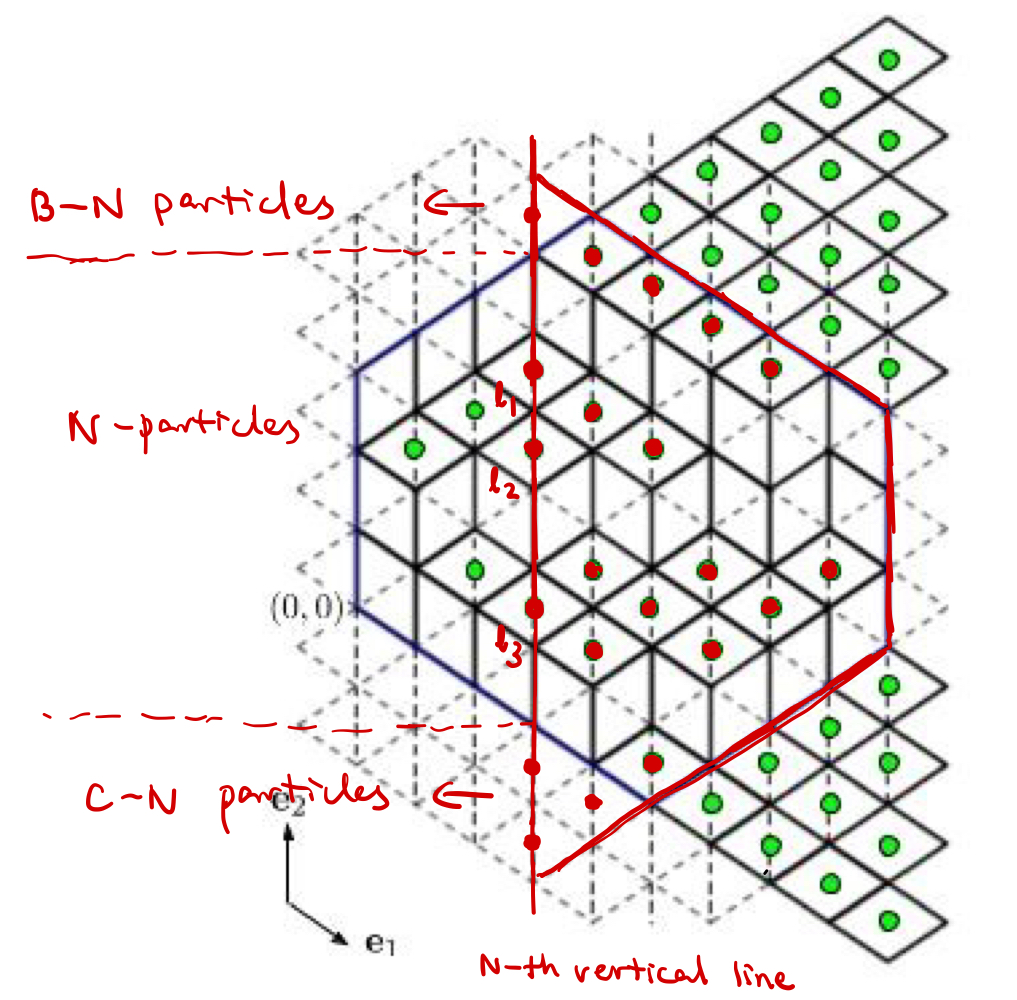
\includegraphics[scale=0.2]{converse-tiling}
	\end{figure}  
	From the picture, we can see the following several facts:
	(\romannumeral 1) Focused on the $n$-th vertical line, the left hand side of it is a tiling from the left to the right, and the right hand side of it is a tiling from the right to the left if we extend the tiling region as the picture does.\\
	(\romannumeral 2) The left hand side(green dots) is a tiling from $(0,0)$ to $(N,\lambda^{\ell})$, while the right hand side(red dots) is a tiling from $(0,0)$ to $(B+C-N,\lambda^{\prime})$, if we look at it in the opposite direction(from the right to the left). Here, $\lambda^{\prime}$ is a new partition that we will investigate in the next paragraph. For now we can easily observe that the extended $N$-$th$ vertical line, or the $(B+C-N)$-$th$ vertical line from the right to the left, contains $B+C-N$ particles. There are $B-N$ particles above and $C-N$ particles below the hexagon region, which are specified in the picture. Also, the hexagon region contains $N$ particles of the original tiling from the left to the right.\\
	(\romannumeral 3) From the construction of the tiling and the ``converse tiling'' in the opposite direction, we can find that there is a bijection between tiling from $(N,\lambda^{\ell})$ to $(B+C,\mu)$ and tiling from $(0,0)$ to $(B+C-N,\lambda^{\prime})$. Therefore, to compute the number of tilings from $(N,\lambda^{\ell})$ to $(B+C,\mu)$ is equivalent to compute the number of tilings from $(0,0)$ to $(B+C-N,\lambda^{\prime})$.\\
	\par Next, let's find the new partition $\lambda^{\prime}$. In the following proof, we consider the ``converse tiling'' and use the corresponding coordinates. We denote the second coordinates of the particles on the $(B+C-N)$-$th$ vertical line by $y^{B+C-N}_{i}$ from the top to the bottom, $i=1,2,\dots,B+C-N$. Denote $\ell^{\prime}_{i}=y^{B+C-N}_{i}-\frac{1}{2}$, and it's easy to check: 
	$$
	\ell^{\prime}_{i}=
	\begin{cases}
	A+B+C-N-i, &\text{if $1\leqslant i\leqslant B-N$;} \\
	\ell_{i-(B-N)}+C-N, &\text{if $B-N+1\leqslant i\leqslant B$;}\\
	B+C-N-i, &\text{if $B+1\leqslant i\leqslant B+C-N$;}
	\end{cases}
	$$
	Define $\lambda_{i}^{\prime}=\ell_{i}^{\prime}-(B+C-N-i)$, $i=1,2,\dots,B+C-N$, and it is not difficult to check:
	$$
	\lambda^{\prime}_{i}=
	\begin{cases}
	A, &\text{if $i\in I_{1}$;} \\
	\ell_{i-(B-N)}-B+i, &\text{if $i\in I_{2}$;}\\
	0, &\text{if $i\in I_{3}$;}
	\end{cases}
	$$
	where $I_{1}=\llbracket{1,B-N}\rrbracket$, $I_{2}=\llbracket{B-N+1,B}\rrbracket$, $I_{3}=\llbracket{B+1,B+C-N}\rrbracket$. We also denote $I=\llbracket{1,N}\rrbracket$ and $T=\llbracket{1,C-N}\rrbracket$. Then we compute the Schur polynomial $$s_{\lambda^{\prime}}(1^{B+C-N})=\prod_{1\leqslant i<j\leqslant B+C-N}\frac{\lambda^{\prime}_{i}-\lambda_{j}^{\prime}+j-i}{j-i}$$
	The product in the above equality can be divided into the following $6$ parts:
	\begin{align*}
	P_{1} &= \prod_{i<j; i,j\in I_{1}}\frac{\lambda_{i}-\lambda_{j}+j-i}{j-i}=\prod_{i<j; i,j\in I_{1}}\frac{A-A+j-i}{j-i}=1\\
	P_{2} &= \prod_{i\in I_{1},j\in I_{2}}\frac{A-(\ell_{j-(B-N)}-B+j)+j-i}{j-i}=\prod_{i\in I_{1},j\in I_{2}}\frac{A-\ell_{j-(B-N)}+B-i}{j-i}\\ 
	&= \prod_{i\in I_{1},j\in I}\frac{A-\ell_{j}+B-i}{j+B-N-i} = \prod_{j\in I}\frac{(A+B-\ell_{j}-1)!/(A+N-\ell_{j}-1)!}{(j+B-N-1)!/(j-1)!}\\
	P_{3}&=\prod_{i\in I_{1},j\in I_{3}}\frac{A-0+j-i}{j-i}=\prod_{i\in I_{1},j\in I_{3}}\frac{A+j-i}{j-i}\\
	P_{4}&=\prod_{i<j;i,j\in I_{2}}\frac{\lambda^{\prime}_{i}-\lambda_{j}^{\prime}+j-i}{j-i}=\prod_{i<j;i,j\in I_{2}}\frac{\ell_{i-(B-N)}-\ell_{j-(B-N)}}{j-i}\\
	&= \prod_{1\leqslant i<j\leqslant N}\frac{\ell_{i}-\ell_{j}}{j-i}=s_{\lambda^{\ell}}(1^{N})\\
	P_{5}&=\prod_{i\in I_{2},j\in I_{3}}\frac{(\ell_{i-(B-N)}-B+i)+j-i}{j-i}=\prod_{i\in I_{2},j\in I_{3}}\frac{\ell_{i-(B-N)}-B+j}{j-i}\\
	&= \prod_{i\in I,j\in T}\frac{\ell_{i}+j}{j-i+N}=\prod_{i\in I}\frac{(\ell_{i}+C-N)!/\ell_{i}!}{(C-i)!/(N-i)!}\\
	P_{6}&=\prod_{i<j; i,j\in I_{3}}\frac{0-0+j-i}{j-i}=1
	\end{align*}
	Notice that only $P_{2}$ and $P_{5}$ contain the term $\ell_{i}$, and we have 
	\begin{align*}
	P_{2}\cdot P_{5} &= \prod_{i=1}^{N}\frac{(A+B-\ell_{i}-1)!(\ell_{i}+C-N)!}{(A+N-\ell_{i}-1)!\ell_{i}!}\cdot\prod_{i=1}^{N}\frac{(i-1)!(N-i)!}{(i+B-N-1)!(C-i)!}\\
	&=\Big[\prod_{i=1}^{N}\omega(\ell_{i})\Big]\cdot M
	\end{align*} 
	where $$M=\prod_{i=1}^{N}\frac{(i-1)!(N-i)!}{(i+B-N-1)!(C-i)!}$$ and $$\omega(\ell_{i})=\frac{(A+B-\ell_{i}-1)!(\ell_{i}+C-N)!}{(A+N-\ell_{i}-1)!\ell_{i}!}$$
	To sum up,
	\begin{align*}
	\mathbb P(\ell_1,\cdots \ell_N)&=\frac{s_{\lambda^{\ell}}(1^{N})\prod_{k=1}^{6}P_{k}}{s_{\mu}(1^{B+C})}=\frac{(s_{\lambda^{\ell}}(1^{N}))^{2}\cdot P3\cdot P2\cdot P5}{s_{\mu}(1^{B+C})}\\
	&=\prod_{1\leqslant i<j\leqslant N}\frac{(\ell_{i}-\ell_{j})^{2}}{(j-i)^{2}}\cdot\Big[\prod_{i=1}^{N}\omega(\ell_{i})\Big]\cdot M\cdot P_{3}\cdot\frac{1}{s_{\mu}(1^{B+C})}\\
	&=\frac{1}{Z}\prod_{1\leqslant i <j\leqslant N}(\ell_{i}-\ell_{j})^{2}\prod_{i=1}^{N}\omega(\ell_{i})
	\end{align*}
	where
	\begin{align*}
	Z^{-1}=\frac{M\cdot P_{3}}{s_{\mu}(1^{B+C})}\prod_{1\leqslant i<j\leqslant N}\frac{1}{(j-i)^{2}}
	\end{align*}
	and the expression of $M$, $s_{\mu}(1^{B+C})$, $P_{3}$, and $\omega(\ell_{i})$ are given above.
	
\subsection*{Problem 12}
\textbf{Step 1:} Denote $X_{i}=\frac{\ell_{i}-d_{1}L}{d_{2}\sqrt{L}}$. Take real numbers $u_{1},\dots, u_{N}$ and $v_{1},\dots, v_{N}$ such that $u_{i}<v_{i}$ for $i=1,\dots, N$, and consider the probability: 
\begin{align*}
\mathbb{P}(u_{1}\leqslant X_{1} \leqslant v_{1}, \dots,  u_{N}\leqslant X_{N} \leqslant v_{N})=\mathbb{P}(u_{i}d_{2}\sqrt{L}+d_{1}L\leqslant \ell_{i} \leqslant v_{i}d_{2}\sqrt{L}+d_{1}L, i=1,\dots, N)	
\end{align*}
Denote $m_{i}^{L}=\lfloor u_{i}d_2\sqrt{L}+d_{1}L\rfloor+1$ and $m_{i}^{L}=\lfloor v_{i}d_2\sqrt{L}+d_{1}L\rfloor$. Since $\ell_{i}$'s can only take integer values, the probability can be written as:
\begin{align*}
\mathbb{P}(u_{i}\leqslant X_{i} \leqslant v_{i}, i=1, \dots, N)&=\sum_{t^{(1)}=m_{1}^{L}}^{M_{1}^{L}}\dots\sum_{t^{(N)}=m_{N}^{L}}^{M_{N}^{L}}\mathbb{P}(\ell_{1}=t^{(1)},\dots,\ell_{N}=t^{(N)}) \\&= \sum_{t^{(1)}=m_{1}^{L}}^{M_{1}^{L}}\dots\sum_{t^{(N)}=m_{N}^{L}}^{M_{N}^{L}}\mathbb{P}(X_{1}=\frac{t^{(1)}-d_{1}L}{d_{2}\sqrt{L}},\dots,X_{N}=\frac{t^{(N)}-d_{1}L}{d_{2}\sqrt{L}})\\
&= \sum_{t^{(1)}=m_{1}^{L}}^{M_{1}^{L}}\dots\sum_{t^{(N)}=m_{N}^{L}}^{M_{N}^{L}}\mathbb{P}(X_{1}=s_{t^{(1)}},\dots,X_{N}=s_{t^{(N)}})
\end{align*}
where $s_{t^{(i)}}=\frac{t^{(i)}-d_{1}L}{d_{2}\sqrt{L}}$, and $s_{t^{(i)}}-s_{t^{(i)}-1}=\frac{1}{d_{2}\sqrt{L}}$ for every $m_{i}^{L}+2\leqslant t^{(i)}\leqslant M_{i}^{L}$ and every $i=1,\dots, N$.\\
\textbf{We claim that}, we can find proper values for $d_1$ and $d_{2}$, such that $(d_{2}\sqrt{L})^{N}\mathbb{P}(X_{1}=s_{t^{(1)}},\dots,X_{N}=s_{t^{(N)}})\rightarrow \rho(s_{t^{(1)}},\dots, s_{t^{(N)}})$ as $L\rightarrow\infty$, where $$\rho(x_1,\dots, x_{N})=\frac{1}{(2\pi)^{\frac{N}{2}}\prod_{j=0}^{N-1}(j!)}\prod_{1\leqslant i<j\leqslant N}(x_{i}-x_{j})^2\prod_{i=1}^{N}e^{-\frac{x_{i}^2}{2}}$$ 
Notice that $\rho(x_1,\dots, x_{N})$ is a probability density function because it integrates to $1$ over $\mathbb{R}^{N}$ by Selberg's Integral(\emph{Corollary 2.5.9, Random Matrix, Zeitouni}). We'll prove this claim in Step $2$ and $3$.\\
If our claim holds, then
\begin{align*}
	\mathbb{P}(u_{i}\leqslant X_{i} \leqslant v_{i}, i=1, \dots, N)&=\sum_{t^{(1)}=m_{1}^{L}}^{M_{1}^{L}}\dots\sum_{t^{(N)}=m_{N}^{L}}^{M_{N}^{L}}(\frac{1}{d_{2}\sqrt{L}})^{N}(\rho(s_{t^{(1)}},\dots, s_{t^{(N)}})+o(1))\\
	&\approx \sum_{t^{(1)}=m_{1}^{L}}^{M_{1}^{L}}\dots\sum_{t^{(N)}=m_{N}^{L}}^{M_{N}^{L}}\int_{s_{t^{(1)}}-\frac{1}{2d_{2}\sqrt{L}}}^{s_{t^{(1)}}+\frac{1}{2d_{2}\sqrt{L}}}\dots\int_{s_{t^{(N)}}-\frac{1}{2d_{2}\sqrt{L}}}^{s_{t^{(N)}}+\frac{1}{2d_{2}\sqrt{L}}}\rho(x_1,\dots, x_{N})dx_{1}\dots dx_{N}\\
	& = \int_{s_{m^{L}_{1}}-\frac{1}{2d_{2}\sqrt{L}}}^{s_{M^{L}_{1}}+\frac{1}{2d_{2}\sqrt{L}}}\dots\int_{s_{m^{L}_{N}}-\frac{1}{2d_{2}\sqrt{L}}}^{s_{M^{L}_{N}}+\frac{1}{2d_{2}\sqrt{L}}}\rho(x_1,\dots, x_{N})dx_{1}\dots dx_{N}\\
	& \rightarrow \int_{u_{1}}^{v_{1}}\dots\int_{u_{N}}^{v_{N}}\rho(x_1,\dots, x_{N})dx_{1}\dots dx_{N}
\end{align*}
where the approximation in the second line uses the definition of Riemann integral.
Let $u_{i}\rightarrow -\infty$, we get $$\mathbb{P}(X_{i} \leqslant v_{i}, i=1, \dots, N)\xrightarrow{L\rightarrow\infty} \int_{-\infty}^{v_{1}}\dots\int_{-\infty}^{v_{N}}\rho(x_1,\dots, x_{N})dx_{1}\dots dx_{N}$$ which means the random vector $(X_{1},\dots,X_{N})$ weakly converges to a continuous distribution with density $\rho(x_{1},\dots,x_{N})$.\\
\textbf{Step 2:} Now we start to prove our claim. In this step, we do some further computation about normalized constant $Z$ based on Problem 11.
From Problem 11 we know:
\begin{align*}
	Z=\frac{M\cdot P_{3}}{s_{\mu}(1^{B+C})}\prod_{1\leqslant i<j\leqslant N}\frac{1}{(j-i)^{2}}
\end{align*}
Compute each part:
\begin{align*}
	P_{3} &= \prod_{i\in I_{1},j\in I_{3}}\frac{A+j-i}{j-i} = \prod_{i=1}^{B-N}\frac{(A+B+C-N-i)!/(A+B-i)!}{(B+C-N-i)!/(B-i)!}\\ &=\prod_{j=0}^{B-N-1}\frac{(A+C+j)!(N+j)!}{(C+j)!(A+N+j)!}\quad(\text{let $j=B-N-i$})\\
	M &=\prod_{i=1}^{N}\frac{(i-1)!(N-i)!}{(B-N+i-1)!(C-i)!}\\
	s_{\mu}(1^{B+C})&=\prod_{i=1}^{C}\prod_{j=C+1}^{B+C}\frac{A+j-i}{j-i}=\prod_{i=1}^{C}\frac{(A+B+C-i)!/(A+C-i)!}{(B+C-i)!/(C-i)!}\\ &= \prod_{j=0}^{C-1}\frac{(A+B+j)!j!}{(A+j)!(B+j)!}\quad(\text{let $j=C-i$})
\end{align*}
Notice that the product of two terms---$\prod_{j=0}^{B-N-1}(A+C+j)!$ in $P_{3}$ and $\prod_{j=0}^{C-1}(A+j)!$ in $s_{\mu}(1^{B+C})$, is $\prod_{j=0}^{B+C-N-1}(A+j)!$, and similarly we can corporate other terms in $P_{3}$ and $s_{\mu}(1^{B+C})$ ($(N+j)!$ in $P_{3}$ and $(B+j)!$ in $s_{\mu}(1^{B+C})$; $(C+j)!$ in $P_{3}$ and $j!$ in $s_{\mu}(1^{B+C})$; $(A+N+j)!$ in $P_{3}$ and $(A+B+j)!$ in $s_{\mu}(1^{B+C})$), and we finally get: 
\begin{align*}
	\frac{P_{3}}{s_{\mu}(1^{B+C})}&=\prod_{i=0}^{B+C-N-1}\frac{(A+i)!(N+i)!}{i!(A+N+i)!}=\prod_{i=0}^{B+C-N-1}\frac{i+1}{i+A+1}\cdot\frac{i+2}{A+i+2}\dots\frac{i+N}{i+A+N}\\
	&= \prod_{i=0}^{B+C-N-1}\prod_{k=1}^{N}\frac{i+k}{i+A+k}=\prod_{k=1}^{N}\frac{(B+C-N-1+k)!/(k-1)!}{(A+B+C-N-1+k)!/(A+k-1)!}\\ &= \prod_{k=1}^{N}\frac{(B+C-N-1+k)!(A+k-1)!}{(A+B+C-N-1+k)!}\cdot\prod_{j=0}^{N-1}\frac{1}{j!}
\end{align*}
Note that the numerator of $M$ is actually $\prod_{j=0}^{N-1}(j!)^{2}$, which cancel the $\prod_{1\leqslant i<j\leqslant N}\frac{1}{(j-i)^{2}}$ in the expression of $Z^{-1}$. Therefore, 
\begin{align*}
	Z^{-1}&=\frac{M\cdot P_{3}}{s_{\mu}(1^{B+C})}\prod_{1\leqslant i<j\leqslant N}\frac{1}{(j-i)^{2}}=\frac{M\cdot P_{3}}{s_{\mu}(1^{B+C})}\prod_{j=0}^{N-1}\frac{1}{(j!)^2}\\
	&= \prod_{i=1}^{N}\frac{(B+C-N-1+i)!(A+i-1)!}{(A+B+C-N-1+i)!(B-N+i-1)!(C-i)!}\prod_{j=0}^{N-1}\frac{1}{j!}:= K\cdot\prod_{j=0}^{N-1}\frac{1}{j!}
\end{align*}
Now we further compute $K$. We extract out the smallest factorial in each of these products of factorials:
\begin{align*}
	&\prod_{i=1}^{N}(A+i-1)!=(A!)^{N}\prod_{i=1}^{N-1}\prod_{j=1}^{i}(A+j)\\
	&\prod_{i=1}^{N}(B+C-N+i-1)!=(B+C-N!)^{N}\prod_{i=1}^{N-1}\prod_{j=1}^{i}(B+C-N+j)\\
	&\prod_{i=1}^{N}(A+B+C-N+i-1)!=((A+B+C-N)!)^{N}\prod_{i=1}^{N-1}\prod_{j=1}^{i}(A+B+C-N+j)\\
	&\prod_{i=1}^{N}(B-N+i-1)!=((B-N)!)^{N}\prod_{i=1}^{N-1}\prod_{j=1}^{i}(B-N+j)\\
	&\prod_{i=1}^{N}(C-i)!=((C-N)!)^{N}\prod_{i=1}^{N-1}\prod_{j=1}^{i}(C-N+j)\\
	\end{align*}
Therefore, $K$ can be written as: $$K=\Big[\frac{(B+C-N)!A!}{(B-N)!(C-N)!(A+B+C-N)!}\Big]^{N}\prod_{i=1}^{N-1}\prod_{j=1}^{i}\frac{(B+C-N+j)(A+j)}{(B-N+j)(C-N+j)(A+B+C-N+j)}$$
Since $A=\lfloor aL \rfloor$, $B=\lfloor bL \rfloor$, $C=\lfloor cL \rfloor$, when $L\rightarrow\infty$, we have:
$$\prod_{i=1}^{N-1}\prod_{j=1}^{i}\frac{(B+C-N+j)(A+j)}{(B-N+j)(C-N+j)(A+B+C-N+j)}\rightarrow\Big[\frac{a(b+c)}{bc(a+b+c)}L^{-1}\Big]^{\frac{N(N-1)}{2}}$$
By Stirling's Formula,
\begin{align*}
	&\frac{(B+C-N)!A!}{(A+B+C-N)!} \sim \frac{\sqrt{2\pi}\sqrt{B+C-N}(B+C-N)^{B+C-N}e^{-(B+C-N)}\sqrt{2\pi}\sqrt{A}(A)^{A}e^{-A}}{\sqrt{2\pi}\sqrt{A+B+C-N}(A+B+C-N)^{A+B+C-N}e^{-(A+B+C-N)}}\\
	&= \sqrt{2\pi}\sqrt{\frac{A(B+C-N)}{A+B+C-N}} (\frac{B+C-N}{A+B+C-N})^{B+C-N}(\frac{A}{A+B+C-N})^{A}\\
	&\sim \sqrt{2\pi}\sqrt{\frac{a(b+c)}{a+b+c}}\cdot\sqrt{L}\cdot \\ & exp\{(B+C-N)ln(B+C-N)+AlnA-(A+B+C-N)ln(A+B+C-N)\}
\end{align*}
Note that 
\begin{align*}
	(B+C-N)ln(B+C-N)&=(B+C-N)ln(1-\frac{N}{B+C})+(B+C-N)ln(B+C)\\
	 &\sim (B+C-N)(-\frac{N}{B+C})+(B+C)ln(B+C)-Nln(B+C)\\
	 & \sim -N+(b+c)L\cdot ln((b+c)L)-Nln((b+c)L)
\end{align*}
Similarly, $AlnA\sim aL\cdot ln(aL)$, and $(A+B+C-N)ln(A+B+C-N)\sim -N+(a+b+c)L\cdot ln((a+b+c)L)-Nln((a+b+c)L)$. Then
$$ \frac{(B+C-N)!A!}{(A+B+C-N)!} \sim \sqrt{2\pi}\sqrt{\frac{a(b+c)}{a+b+c}}(alna+(b+c)ln(b+c)-(a+b+c)ln(a+b+c))\cdot L+N\cdot ln(\frac{a+b+c}{b+c})$$
Following this procedure, we compute another quantity:
\begin{align*}
&\frac{(B-N)!(C-N)!}{(B+C-2N)!} \sim \sqrt{2\pi}\sqrt{\frac{bc}{b+c}}\sqrt{L}\cdot exp\{(blnb+clnc-(b+c)ln(b+c))\cdot L+N\cdot ln\frac{(b+c)^{2}}{bc}\}
\end{align*}
Therefore, $$\Big[\frac{(B+C-N)!A!(B+C-2N)!}{(B-N)!(C-N)!(A+B+C-N)!}\Big] \sim \sqrt{\frac{a(b+c)^{2}}{bc(a+b+c)}}\cdot exp\{(S_{0}(a,b,c))\cdot L+N\cdot ln(\frac{bc(a+b+c)}{(b+c)^{3}})\}$$
where $S_{0}(a,b,c)=alna+(b+c)ln(b+c)-(a+b+c)ln(a+b+c)-blnb-clnc+(b+c)ln(b+c)$.
Using Stirling's formula to $(B+C-2N)!$ we get:
$$(B+C-2N)!\sim \sqrt{2\pi}\sqrt{b+c}\sqrt{L}\cdot exp\{-2N+(b+c)L\cdot ln((b+c)L)-2Nln((b+c)L)-(B+C-2N)\}$$
Then,
\begin{align*}
	&\frac{(B+C-N)!A!}{(B-N)!(C-N)!(A+B+C-N)!}=\Big[\frac{(B+C-N)!A!(B+C-2N)!}{(B-N)!(C-N)!(A+B+C-N)!}\Big]/(B+C-2N)!\\
	&\sim (2\pi)^{-\frac{1}{2}}\sqrt{\frac{a(b+c)}{bc(a+b+c)}}\cdot L^{-\frac{1}{2}}\cdot exp\{S_{1}(a,b,c)\cdot L-(b+c)L\cdot lnL+2N+2Nln((b+c)L)\\
	&+(B+C-2N)+N\cdot ln(\frac{bc(a+b+c)}{(b+c)^3})\}
\end{align*}
where $S_{1}(a,b,c)=alna+(b+c)ln(b+c)-(a+b+c)ln(a+b+c)-blnb-clnc$.
Combining the computation above, we get:
\begin{align*}
	K &\sim \Big[\frac{(B+C-N)!A!}{(B-N)!(C-N)!(A+B+C-N)!}\Big]^{N}\Big[\frac{a(b+c)}{bc(a+b+c)}L^{-1}\Big]^{\frac{N(N-1)}{2}}\\
	&\sim (2\pi)^{-\frac{N}{2}}\Big[\sqrt{\frac{a(b+c)}{bc(a+b+c)}}\Big]^{N}\cdot L^{-\frac{N}{2}}\cdot (exp\{P(a,b,c,N,L)\})^{N}\cdot\Big[\frac{a(b+c)}{bc(a+b+c)}L^{-1}\Big]^{\frac{N(N-1)}{2}}\\
	&= \sim (2\pi)^{-\frac{N}{2}}\Big[\sqrt{\frac{a(b+c)}{bc(a+b+c)}}L^{-\frac{1}{2}}\Big]^{N^2}\cdot (exp\{P(a,b,c,N,L)\})^{N}
\end{align*}
where $P(a,b,c,N,L)=S_{1}(a,b,c)\cdot L-(b+c)L\cdot lnL+2Nln((b+c)L)+(B+C)+N\cdot ln(\frac{bc(a+b+c)}{(b+c)^3})$.\\
\textbf{Step 3:} In this step, we find the proper $d_{1}$ and $d_{2}$ and prove our claim.\\
In Problem 11, we get $$\omega(\ell_{i})=\frac{(A+B-\ell_{i}-1)!(\ell_{i}+C-N)!}{(A+N-\ell_{i}-1)!\ell_{i}!}$$ Using Stirling's formula, we obtain:
\begin{align*}
	\omega(\ell_{i})&\sim \sqrt{\frac{(A+B-\ell_{i}-1)(\ell_{i}+C-N)}{(A+N-\ell_{i}-1)\ell_{i}}}\cdot exp\{(A+B-\ell_{i}-1)ln(A+B-\ell_{i}-1)\\ 
	& + (\ell_{i}+C-N)ln(\ell_{i}+C-N)-(A+N-\ell_{i}-1)ln(A+N-\ell_{i}-1)-\ell_{i}ln(\ell_{i})\\
	& -(B+C-2N)\}
\end{align*}
Since $\ell_{i}=x_{i}d_{2}\sqrt{L}+d_{1}L$, $A=\lfloor aL \rfloor$, $B=\lfloor bL \rfloor$, $C=\lfloor cL \rfloor$, when $l\rightarrow\infty$, we have $$\sqrt{\frac{(A+B-\ell_{i}-1)(\ell_{i}+C-N)}{(A+N-\ell_{i}-1)\ell_{i}}}\rightarrow \sqrt{\frac{(a+b-d_{1})(c+d_{1})}{(a-d_{1})d_{1}}}$$
For the terms in the exponent, we first get rid of all the constants(using Taylor's expansion):
\begin{align*}
	&(A+B-\ell_{i}-1)ln(A+B-\ell_{i}-1)\sim (A+B-\ell_{i})ln(A+B-\ell_{i})-ln(A+B-\ell_{i})-1\\
	& (\ell_{i}+C-N)ln(\ell_{i}+C-N)\sim (\ell_{i}+C)ln(\ell_{i}+C)-Nln(\ell_{i}+C)-N\\
	& (A+N-\ell_{i}-1)ln(A+N-\ell_{i}-1)\sim (A-\ell_{i})ln(A-\ell_{i})+(N-1)ln(A-\ell_{i})+(N-1)
\end{align*}
Notice that
\begin{align*}
	& A+B-\ell_{i} = (a+b-d_1)L-x_{i}d_{2}\sqrt{L}+O(1)
\end{align*}
and 
\begin{align*}
	ln(A+B-\ell_{i}) &= ln(a+b-d_1)L+ln(1-\frac{x_{i}d_{2}}{(a+b-d_{1})\sqrt{L}}+O(\frac{1}{L}))\\
	&= ln(a+b-d_1)L - \frac{x_{i}d_{2}}{(a+b-d_{1})\sqrt{L}}-\frac{1}{2}\frac{x_{i}^2d_{2}^2}{(a+b-d_{1})^2 L} + O(\frac{1}{L})
\end{align*}
Then,
\begin{align*}
	&(A+B-\ell_{i})ln(A+B-\ell_{i})\sim \\
	&(a+b-d_{1})L\cdot ln((a+b-d_{1})L)-d_{2}x_{i}\sqrt{L}+\frac{1}{2}\frac{d_{2}^2 x_{i}^2}{a+b-d_{1}}-d_{2}x_{i}\sqrt{L}\cdot ln((a+b-d_{1})L)
\end{align*}
Similarly, we compute other terms($(A+B-\ell_{i})ln(A+B-\ell_{i})$,$(\ell_{i}+C)ln(\ell_{i}+C)$, $(A-\ell_{i})ln(A-\ell_{i})$, $\ell_{i}ln(\ell_{i})$) in the exponential part of $\omega(\ell_{i})$. Plug them into the formula of $\omega(\ell_{i})$, we get its exponential part:
\begin{align*}
	&exp\{(a+b-d_{1})L\cdot ln((a+b-d_{1})L)+(c+d_{1})L\cdot ln((c+d_{1})L)-(a-d_{1})L\cdot ln((a-d_{1})L)-\\
	& d_{1}L\cdot ln(d_{1}L)-2N-ln((a+b-d_{1})L)-Nln((d_{1}+c)L)-(N-1)ln((a-d_{1})L)-(B+C-2N)\\
	&+d_{2}x_{i}\sqrt{L}ln\frac{(c+d_{1})(a-d_{1})}{(a+b-d_{1})d_{1}}+\frac{1}{2}d_{2}^{2}x_{i}^{2}[\frac{1}{a+b-d_{1}}+\frac{1}{c+d_{1}}-\frac{1}{a-d_{1}}-\frac{1}{d_{1}}]\}
\end{align*}
Let 
\begin{equation*}
\left\{
\begin{array}{lr}
\frac{(c+d_{1})(a-d_{1})}{(a+b-d_{1})d_{1}}=1 &  \\
(\frac{1}{a+b-d_{1}}+\frac{1}{c+d_{1}}-\frac{1}{a-d_{1}}-\frac{1}{d_{1}})d_{2}^2=-1 &
\end{array}	
\right.
\end{equation*}
Solve this equation we get
\begin{equation*}
\left\{
\begin{array}{lr}
d_{1}=\frac{ac}{b+c} &  \\
d_{2}=\sqrt{\frac{abc(a+b+c)}{(b+c)^3}} &
\end{array}	
\right.
\end{equation*}
and we finally get
$$\omega(\ell_{i})\sim \sqrt{\frac{(a+b-d_{1})(c+d_{1})}{(a-d_{1})d_{1}}}exp\{S_{2}(a,b,c,L)-\frac{1}{2}x_{i}^{2}\}=\frac{a+b+c}{a}\cdot exp\{S_{2}(a,b,c,L)-\frac{1}{2}x_{i}^{2}\}$$
where $S_{2}(a,b,c,L)=(a+b-d_{1})L\cdot ln((a+b-d_{1})L)+(c+d_{1})L\cdot ln((c+d_{1})L)-(a-d_{1})L\cdot ln((a-d_{1})L)-d_{1}L\cdot ln(d_{1}L)-ln((a+b-d_{1})L)-Nln((d_{1}+c)L)-(N-1)ln((a-d_{1})L)-(B+C)$.\\
Combining the computation results \textbf{Step 2}, we get
\begin{align*}
	&(d_{2}\sqrt{L})^{N}\mathbb{P}(\ell_{1},\dots,\ell_{N})=(d_{2}\sqrt{L})^{N}\frac{1}{Z}\prod_{1\leqslant i <j\leqslant N}(\ell_{i}-\ell_{j})^{2}\prod_{i=1}^{N}\omega(\ell_{i})\\
	&=(d_{2}\sqrt{L})^{N^2}K\cdot\prod_{j=0}^{N-1}\frac{1}{j!}\Big[\prod_{1\leqslant i <j\leqslant N}(x_{i}-x_{j})^{2}\Big](\frac{a+b+c}{a})^{N}exp\{N\cdot S_{2}(a,b,c,L)\}\cdot\prod_{i=1}^{N}e^{-\frac{x_{i}^{2}}{2}}
\end{align*}
Notice that
\begin{align*}
	&K\cdot(d_{2}\sqrt{L})^{N^2}\cdot exp\{N\cdot S_{2}(a,b,c,L)\} \sim (2\pi)^{-\frac{N}{2}}\Big[\sqrt{\frac{a(b+c)}{bc(a+b+c)}}L^{-\frac{1}{2}}\cdot d_{2}\sqrt{L} \Big]^{N^2}\cdot\\
	& exp\{N(P(a,b,c,N,L)+S_{2}(a,b,c,L))\}
\end{align*}
Plug $d_{1}$ into $S_{2}(a,b,c,L)$ we get:
\begin{align*}
	& S_{2}(a,b,c,L)=\Big[\frac{b(a+b+c)}{b+c}ln(\frac{b(a+b+c)}{b+c})+\frac{c(a+b+c)}{b+c}ln(\frac{c(a+b+c)}{b+c})-\frac{ab}{b+c}ln(\frac{ab}{b+c})\\
	& -\frac{ac}{b+c}ln(\frac{ac}{b+c})\Big]\cdot L+(b+c)\cdot L\cdot lnL -ln(\frac{b(a+b+c)}{b+c})-Nln(d_{1}+c) -(N-1)ln(a-d_{1})\\
	&-2N\cdot lnL-(B+C)
\end{align*}
Add $P(a,b,c,N,L)$ and $S_{2}(a,b,c,L)$, we will find the coefficients of term $L$, $L\cdot LlnL$, and $lnL$ equal to zero. Then, we are left with: 
\begin{align*}
	&P(a,b,c,N,L)+S_{2}(a,b,c,L)= -ln(\frac{b(a+b+c)}{b+c})-Nln(\frac{c(a+b+c)}{b+c})-Nln(\frac{ab}{b+c})+ln(\frac{ab}{b+c})\\
	& +N\cdot ln(\frac{bc(a+b+c)}{(b+c)^3}) = ln(\frac{a}{a+b+c})-Nln(\frac{a}{b+c})
\end{align*}
Therefore, 
\begin{align*}
	&K\cdot(d_{2}\sqrt{L})^{N^2}\cdot exp\{N\cdot S_{2}(a,b,c,L)\} \sim (2\pi)^{-\frac{N}{2}}\Big[\sqrt{\frac{a(b+c)}{bc(a+b+c)}}L^{-\frac{1}{2}}\cdot d_{2}\sqrt{L} \Big]^{N^2}\cdot\\
	& (\frac{a}{a+b+c})^{N}\cdot (\frac{b+c}{a})^{N^2}=(2\pi)^{-\frac{N}{2}}(\frac{a}{a+b+c})^{N}
\end{align*}
Finally, we obtain
\begin{align*}
	&(d_{2}\sqrt{L})^{N}\mathbb{P}(\ell_{1},\dots,\ell_{N})\xrightarrow{L\rightarrow\infty}\frac{1}{(2\pi)^{\frac{N}{2}}\prod_{j=0}^{N-1}(j!)}\prod_{1\leqslant i<j\leqslant N}(x_{i}-x_{j})^2\prod_{i=1}^{N}e^{-\frac{x_{i}^2}{2}}
\end{align*}
Following the logic of \textbf{Step 1}, we conclude that the random vector $(X_{1},\dots,X_{N})$ weakly converges to the continuous distribution with density $\rho(x_{1},\dots,x_{N})$ as given above. In addition, the quantities that the problem requires us to find are: $d_{1}=\frac{ac}{b+c}$, $d_{2}=\sqrt{\frac{abc(a+b+c)}{(b+c)^3}}$, $Z_{N}=(2\pi)^{\frac{N}{2}}\prod_{j=0}^{N-1}(j!)$.

	
	\subsection*{Problem 13}

Define a probability distribution on $N$-tuples as
$$P_N(l_1, \cdots, l_N) = \frac{\omega(l_1, \cdots, l_N)}{Z_N}$$
where $Z_N$ is the sum of the weights
$$\omega(l_1, \cdots, l_N) = \prod_{1 \leq i < j \leq N} (l_i - l_j)^2 \prod_{i = 1}^N \frac{t^{l_i}}{l_i !}$$
Note that this sum is finite, since
$$\sum_{l_1 > l_2 > \cdots > l_n \geq 0} \omega(l_1, \cdots, l_N) \leq \sum_{l_1 = N-1}^\infty l_1^{N^2} \frac{C_1 + A_1^{Nl_1}}{l_1!}$$\\

In the problem, we are given that $A_k, B_k, C_k \in \mathbb{N}$, with $\lim_{k \rightarrow \infty} A_k = \lim_{k \rightarrow \infty} B_k = \lim_{k \rightarrow \infty} C_k = \infty$ and $\lim_{k \rightarrow \infty} \frac{A_k C_k}{B_k} = t$. From problem 11, we have that
$$P(l_1, \cdots, l_N) = \frac{1}{Z} \prod_{1 \leq i < j \leq N} (l_i - l_j)^2 \prod_{i = 1}^N \omega(l_i)$$
where
$$\omega(y) = \frac{(y + C - N)!(A + B - y - 1)!}{y!(A + N - y - 1)!}$$
Now notice that
$$\frac{(y + C_k - N) ! (A_k + B_k - y + 1)!}{y! (A_k + N - y - 1)!}$$
$$= \frac{A_K + B_k - 1)! (C_k - N)!}{(A_k + N - 1)!} \frac{(A_k + N - 1) \cdots (A_k + N - y) (C_k - N + 1)}{y! (A_k + B_k - 1) \cdots (A_k + B_k - y)}$$\\

Hence we can write
$$P_k(l_1, \cdots, l_N) = \frac{1}{Z_k} \prod_{1 \leq i < j \leq N}(l_i - l_j)^2 \prod_{i = 1}^N \omega_k (l_i)$$
where
$$\omega_k(y) = \frac{A_K + B_k - 1)! (C_k - N)!}{(A_k + N - 1)!} \frac{(A_k + N - 1) \cdots (A_k + N - y) (C_k - N + 1)}{y! (A_k + B_k - 1) \cdots (A_k + B_k - y)}$$\\

Notice that $\lim_{k \rightarrow \infty} \omega_k(y) = \frac{t^k}{y!} \forall y$, since 
$$\omega(y) = \frac{(y + C - N)!(A + B - y - 1)!}{y!(A + N - y - 1)!}$$
and
$$\lim_{k \rightarrow \infty} \frac{A_k C_k}{B_k} = t$$\\

Also note that
$$\frac{\omega_k (y+1)}{\omega_k (y)} \leq \frac{1}{2}$$
for $y \geq y_0$, $k\geq k_0$. Hence there exists a constant $C$, s.t. $\omega_k(y) \leq C 2^{-y}$ for $k \geq k_0$, $y \geq y_0$. Combining the last two inequalities, we get that
$$\prod_{1 \leq i <  \leq N} (j - i)^2 \prod_{i = 1}^N \frac{t^i}{i !} \leq \liminf_{k \rightarrow \infty} Z_k \leq \limsup_{k \rightarrow \infty} Z_k \leq \sum_{l_i = N - 1}^\infty l_i^{N^2} C^N 2^{-l_i}..., \forall k$$
so $Z_k$ is bounded uniformly for all $k$.\\

Now, if in addition to $Z_K$ being bounded uniformly, we can show that $P_k$ is a tight sequence of measures, it suffices to show that each subsequential limit is $P_N$ to prove our claim that
$$P_N(l_1, \cdots, l_N) = \frac{\omega(l_1, \cdots, l_N)}{Z_N}$$

Let $\epsilon > 0$ be given. We want to show that the distribution of $l_1$ under $P_k$ is tight. We know that for all $k$, $Z_k < \infty$, $\exists c$, s.t. $Z_k \geq c$ and 
$$\sum_{l_1 = N}^\infty l_1^N C^N 2^{-l_1} C < c \epsilon$$
Then
$$P_k(l_1 \geq M) = \frac{1}{Z_k} \sum_{l_1 > \cdots > l_n > 0, l_1 \geq M} \prod_{1\leq i < j \leq M}(l_i - l_j)^2 \prod_{k = 1}^N \omega_k(l_i) \leq \frac{1}{c} c \epsilon < \epsilon$$
which proves the tightness of $l_1$ under $P_k$.\\

To prove the convergence of every subsequence to $P_N$, we let $k_p$ be a subsequence with $P_{k_p}$ converging weakly to some measure $P'$. If we assume that $Z_{k_p}$ converges to some constant $Z'$, then weak convergence implies that 
$$\lim_{p \rightarrow \infty} P_{k_p} (l_1, \cdots, l_N) = P'(l_1, \cdots, l_N)$$
for all $l_1 > \cdots > l_N \geq 0$. Earlier, we showed that
$$\lim_{k \rightarrow \infty} \omega_k(y) = \frac{t^k}{y!}$$
so that
$$P'(l_1, \cdots, l_N) = \frac{1}{Z'} \prod_{1 \leq i < j \leq N} (l_i - l_j)^2 \prod_{i = 1}^N \frac{t^{l_i}}{l_i !}$$\\

Then $Z' = Z^N$, since $P'$ is a probability measure, so $P'$ is the same as $P^N$, hence all subsequential limits of $P_k$ must be $P^N$. This completes the proof.


\subsection*{Problem 14}
In this problem, we mimic the process in Problem 12 to prove the weak convergence of the random vector $(X_{1},\dots,X_{N})$, where $X_{i}=\frac{\ell_{i}}{n}$, $i=1,\dots,N$. Take real numbers $u_{1},\dots, u_{N}$ and $v_{1},\dots, v_{N}$ such that $u_{i}<v_{i}$ for $i=1,\dots, N$, and consider the probability: 
\begin{align*}
\mathbb{P}(u_{1}\leqslant X_{1} \leqslant v_{1}, \dots,  u_{N}\leqslant X_{N} \leqslant v_{N})&=\mathbb{P}(nu_{i}\leqslant \ell_{i} \leqslant nv_{i}, i=1,\dots, N)	\\
&=\sum_{t^{(1)}=\lfloor nu_{1}\rfloor+1}^{\lfloor nv_{1}\rfloor}\dots \sum_{t^{(N)}=\lfloor nu_{N}\rfloor+1}^{\lfloor nv_{N}\rfloor}\mathbb{P}(\ell_{1}=t^{(1)},\dots,\ell_{N}=t^{(N)})\\
&=\sum_{t^{(1)}=\lfloor nu_{1}\rfloor+1}^{\lfloor nv_{1}\rfloor}\dots \sum_{t^{(N)}=\lfloor nu_{N}\rfloor+1}^{\lfloor nv_{N}\rfloor}\mathbb{P}(X_{1}=s_{t^{(1)}},\dots, X_{N}=s_{t^{(N)}})
\end{align*}
where $s_{t^{(i)}}=\frac{t^{(i)}}{n}$, and $s_{t^{(i)}}-s_{t^{(i)}-1}=\frac{1}{n}$ for every $\lfloor nu_{i}\rfloor +2\leqslant t^{(i)}\leqslant \lfloor nv_{i}\rfloor$ and every $i=1,\dots, N$.\\
\textbf{We claim that}, $(n)^{N}\mathbb{P}(X_{1}=s_{t^{(1)}},\dots,X_{N}=s_{t^{(N)}})\rightarrow \rho(s_{t^{(1)}},\dots, s_{t^{(N)}})$ as $n\rightarrow\infty$, where $$\rho(x_1,\dots, x_{N})=\frac{1}{\prod_{j=0}^{N-1}(j!)^{2}}\prod_{1\leqslant i<j\leqslant N}(x_{i}-x_{j})^2\prod_{i=1}^{N}e^{-x_{i}}\mathbbm{1}_{\{x1,\dots, x_{N}\geqslant 0\}}$$ 
Notice that $\rho(x_1,\dots, x_{N})$ is a probability density function because it integrates to $1$ over $[0,\infty]^{N}$ by Selberg's Integral(\emph{Corollary 2.5.9, Random Matrix, Zeitouni}). We will prove this claim later.\\
Denote $m^{L}_{i}=\lfloor nu_{i}\rfloor+1$, and $M^{L}_{i}=\lfloor nv_{i}\rfloor$. If our claim holds, then
\begin{align*}
\mathbb{P}(u_{i}\leqslant X_{i} \leqslant v_{i}, i=1, \dots, N)&=\sum_{t^{(1)}=m_{1}^{L}}^{M_{1}^{L}}\dots\sum_{t^{(N)}=m_{N}^{L}}^{M_{N}^{L}}(\frac{1}{n})^{N}(\rho(s_{t^{(1)}},\dots, s_{t^{(N)}})+o(1))\\
&\approx \sum_{t^{(1)}=m_{1}^{L}}^{M_{1}^{L}}\dots\sum_{t^{(N)}=m_{N}^{L}}^{M_{N}^{L}}\int_{s_{t^{(1)}}-\frac{1}{2n}}^{s_{t^{(1)}}+\frac{1}{2n}}\dots\int_{s_{t^{(N)}}-\frac{1}{2n}}^{s_{t^{(N)}}+\frac{1}{2n}}\rho(x_1,\dots, x_{N})dx_{1}\dots dx_{N}\\
& = \int_{s_{m^{L}_{1}}-\frac{1}{2n}}^{s_{M^{L}_{1}}+\frac{1}{2n}}\dots\int_{s_{m^{L}_{N}}-\frac{1}{2n}}^{s_{M^{L}_{N}}+\frac{1}{2n}}\rho(x_1,\dots, x_{N})dx_{1}\dots dx_{N}\\
& \rightarrow \int_{u_{1}}^{v_{1}}\dots\int_{u_{N}}^{v_{N}}\rho(x_1,\dots, x_{N})dx_{1}\dots dx_{N}
\end{align*}
where the approximation in the second line uses the definition of Riemann integral.
Let $u_{i}\rightarrow -\infty$, we get $$\mathbb{P}(X_{i} \leqslant v_{i}, i=1, \dots, N)\xrightarrow{n\rightarrow\infty} \int_{-\infty}^{v_{1}}\dots\int_{-\infty}^{v_{N}}\rho(x_1,\dots, x_{N})dx_{1}\dots dx_{N}$$ which means the random vector $(X_{1},\dots,X_{N})$ weakly converges to a continuous distribution with density $\rho(x_{1},\dots,x_{N})$.\\
Now we prove our previous claim. By Cauchy identity, we have $$\sum_{\lambda}s_{\lambda}(a^{N})s_{\lambda}(b^{N})=\prod_{1\leqslant i,j\leqslant N}(1-ab)^{-1}=(1-ab)^{-N^2}$$ Therefore, the normalized constant $Z_{N}(a,b)$ in the problem equals to $(1-ab)^{-N^2}$. By Problem 4, Schur symmetric function is a homogeneous polynomial with degree $|\lambda|$. Thus, $s_{\lambda}(a^{N})=a^{\sum_{i=1}^{N}\lambda_{i}}s_{\lambda}(1^{N})$ and $s_{\lambda}(b^{N})=b^{\sum_{i=1}^{N}\lambda_{i}}s_{\lambda}(1^{N})$. Then,
\begin{align*}
\mathbb{P}(\lambda)&= (1-ab)^{N^2}\cdot s_{\lambda}(a^{N})\cdot s_{\lambda}(b^{N})=(1-ab)^{N^2}(ab)^{\sum_{i=1}^{N}\lambda_{i}}(s_{\lambda}(1^{N}))^{2}\\
&=(1-ab)^{N^2}(ab)^{\sum_{i=1}^{N}(\ell_{i}+i-N)}\prod_{1\leqslant i<j\leqslant N}\Big[\frac{\lambda_{i}-\lambda_{j}+j-i}{j-i}\Big]^{2}\\
&=(1-ab)^{N^2}(ab)^{(\sum_{i=1}^{n}\ell_{i})-\frac{1}{2}N(N-1)}\prod_{1\leqslant i<j\leqslant N}\Big[\frac{\ell_{i}-\ell_{j}}{j-i}\Big]^{2}\\
&=(1-ab)^{N^2}(ab)^{-\frac{1}{2}N(N-1)}\prod_{i=0}^{N-1} \frac{1}{(j!)^{2}}\cdot \prod_{1\leqslant i<j\leqslant N}(\ell_{i}-\ell_{j})^{2}\cdot\prod_{i=1}^{N}(ab)^{\ell_{i}}
\end{align*}
Moreover,
\begin{align*}
&(n)^{N}\mathbb{P}(X_{1}=s_{t^{(1)}},\dots,X_{N}=s_{t^{(N)}})=(n)^{N}\mathbb{P}(\ell_{1}=t^{(1)},\dots,\ell_{N}=t^{(N)})\\
&= n^{N}(1-ab)^{N^2}(ab)^{-\frac{1}{2}N(N-1)}\prod_{i=0}^{N-1} \frac{1}{(j!)^{2}}\cdot \prod_{1\leqslant i<j\leqslant N}(t^{(i)}-t^{(j)})^{2}\cdot\prod_{i=1}^{N}(ab)^{t_{(i)}}\\
&= n^{N}(1-e^{-\frac{1}{n}})^{N^2}(e^{-\frac{1}{n}})^{-\frac{1}{2}N(N-1)}\prod_{i=0}^{N-1}\frac{1}{(j!)^2}\prod_{1\leqslant i<j\leqslant N}(s_{t^{(i)}}-s_{t^{(j)}})^{2}\cdot n^{N(N-1)}\cdot\prod_{i=1}^{N}e^{-\frac{t^{(i)}}{n}}\\
&= K \prod_{i=0}^{N-1}\frac{1}{(j!)^2}\prod_{1\leqslant i<j\leqslant N}(s_{t^{(i)}}-s_{t^{(j)}})^{2}\prod_{i=1}^{N}e^{-s_{t^{(i)}}}
\end{align*}
where $K=n^{N^2}(1-e^{-\frac{1}{n}})^{N^2}(e^{-\frac{1}{n}})^{-\frac{1}{2}N(N-1)}$. Denote $x=e^{-\frac{1}{n}}$, then $$K=(1-x)^{N^2}x^{-\frac{1}{2}N(N-1)}(-\frac{1}{lnx})^{N^2}=x^{-\frac{1}{2}N(N-1)}(\frac{x-1}{lnx})^{N^2}$$ When $n\rightarrow\infty$, we have $x\rightarrow 1$ and $K\rightarrow 1$. Thus $(n)^{N}\mathbb{P}(X_{1}=s_{t^{(1)}},\dots,X_{N}=s_{t^{(N)}})\rightarrow\rho(s_{t^{(1)}},\dots,s_{t^{(N)}})$, and we proved our claim. In addition, the two quantities that the problem requires us to find are: $V(x)=x$ and $Z_{N}=\prod_{i=0}^{N-1}\frac{1}{(j!)^2}$.


\section{Couplings}

	\subsection*{Problem 15}
	
	We will prove the following lemma, of which the two lemmas 3.1 and 3.2 are immediate consequences. In particular, Lemma 3.1 is the special case when $g^b = g^t$, and Lemma 3.2 is the case when $\vec{x} = \vec{x}'$ and $\vec{y} = \vec{y}'$. We argue in analogy to Lemma 5.6 in Dimitrov-Matestki.
	
	\begin{lemma*}
		Fix $k \in \mathbb{N}$, $T_0, T_1 \in \mathbb{Z}$ with $T_0 < T_1$, and two functions $g^b, g^t: \llbracket T_0, T_1 \rrbracket  \rightarrow [-\infty, \infty)$ with $g^b\leq g^t$. Also fix $\vec{x}, \vec{y}, \vec{x}', \vec{y}' \in \mathfrak{W}_k$, such that $g^b(T_0)\leq x_i$, $g^b(T_1)\leq y_i$, $g^t(T_0)\leq x_i'$, $g^t(T_1)\leq y_i'$, and $x_i\leq x_i'$, $y_i\leq y_i'$ for $1\leq i\leq k$. Assume that $\Omega_{avoid}(T_0, T_1, \vec{x}, \vec{y}, \infty,g^b)$ and $\Omega_{avoid}(T_0, T_1, \vec{x}', \vec{y}', \infty,g^t)$ are both non-empty. Then there exists a probability space $(\Omega, \mathcal{F}, \mathbb{P})$, which supports two $\llbracket 1, k \rrbracket$-indexed Bernoulli line ensembles $\mathfrak{L}^t$ and $\mathfrak{L}^b$ on $\llbracket T_0, T_1 \rrbracket$ such that the law of $\mathfrak{L}^{t}$ {\big (}resp. $\mathfrak{L}^b${\big )} under $\mathbb{P}$ is given by $\mathbb{P}_{avoid, Ber}^{T_0, T_1, \vec{x}', \vec{y}', \infty, g^t}$ {\big (}resp. $\mathbb{P}_{avoid, Ber}^{T_0, T_1, \vec{x}, \vec{y}, \infty, g^b}${\big )} and such that $\mathbb{P}$-almost surely we have $\mathfrak{L}_i^t(r) \geq \mathfrak{L}^b_i(r)$ for all $i = 1,\dots, k$ and $r \in \llbracket T_0, T_1 \rrbracket$.
	\end{lemma*}

	\begin{proof} We split the proof into two steps.\\
	
	\textbf{Step 1.} We first aim to construct a Markov chain $(X^n,Y^n)_{n\geq 0}$, with \\$X^n\in \Omega_{avoid}(T_0,T_1,\vec{x},\vec{y},\infty,g^b)$, $Y^n\in \Omega_{avoid}(T_0,T_1,\vec{x}',\vec{y}',\infty,g^t)$, with initial distribution given by the maximal paths
	\begin{align*}
	& X^0_1(t)=(x_1+t-T_0) \wedge y_1,\quad && Y^0_1(t)=(x_1'+t-T_0) \wedge y_1'\\
	& X^0_k(t)=(x_k+t-T_0) \wedge y_k \wedge X^0_{k-1}(t), \quad && Y^0_k(t)=(x_k'+t-T_0) \wedge y_k' \wedge Y^0_{k-1}(t).
	\end{align*}
	for $t\in\llbracket T_0, T_1\rrbracket$. We want this chain to have the following properties: 
	\begin{enumerate}[label=(\arabic*)]
		
		\item $(X^n)_{n\geq 0}$ and $(Y^n)_{n\geq 0}$ are both Markov in their own filtrations,
		
		\item $(X^n)$ is irreducible and has as an invariant distribution the uniform measure $\mathbb{P}_{avoid,Ber}^{T_0,T_1,\vec{x},\vec{y},\infty,g^b}$,
		
		\item $(Y^n)$ is irreducible and has invariant distribution $\mathbb{P}_{avoid,Ber}^{T_0,T_1,\vec{x}',\vec{y}',\infty,g^t}$,
		
		\item $X^n_i\leq Y^n_i$ on $\llbracket T_0, T_1\rrbracket$ for all $n\geq 0$ and $1\leq i \leq k$.
		
	\end{enumerate}

	\noindent This will allow us to conclude convergence of $X^n$ and $Y^n$ to these two uniform measures.
	
	We specify the dynamics of $(X^n, Y^n)$ as follows. At time $n$, we uniformly sample a segment $\{t\}\times[z, z+1]$, with $t\in\llbracket T_0, T_1\rrbracket$ and $z\in\llbracket x_k,y_1'-1\rrbracket$. We also flip a fair coin, with $\mathbb{P}(\textrm{heads})=\mathbb{P}(\textrm{tails})=1/2$. We update $X^n$ and $Y^n$ using the following procedure. For all points $s\neq t$, we set $X^{n+1}(s) = X^n(s)$. If $T_0 < t < T_1$ and $X^n_i(t-1)=z$ and $X^n_i(t+1)=z+1$ (note that this implies $X^n_i(t)\in\{z,z+1\}$), then we set
	\[
	X^{n+1}_i(t) = \begin{cases}
		z+1, & \textrm{if heads},\\
		z, & \textrm{if tails},
	\end{cases}
	\]
	assuming that this move does not cause $X^{n+1}_i(t)$ to fall below $g^b(t)$. In all other cases, we leave $X^{n+1}_i(t)=X^n_i(t)$. We update $Y^n$ using the same rule, with $g^t$ in place of $g^b$. [Maybe add a figure here.] We will verify below in the proof of (4) that $X^n$ and $Y^n$ are in fact non-intersecting for all $n$, but we assume this for now.
	
	It is easy to see that $(X^n,Y^n)$ is a Markov chain, since at each time $n$, the value of $(X^{n+1},Y^{n+1})$ depends only on the current state $(X^n,Y^n)$, and not on the time $n$ or any of the states prior to time $n$. Moreover, the value of $X^{n+1}$ depends only on the state $X^n$, not on $Y^n$, so $(X^n)$ is a Markov chain in its own filtration. The same applies to $(Y^n)$. This proves the property (1) above.
	
	We now argue that $(X^n)$ is each irreducible. Observe that the initial distribution $X^0$ is by construction maximal, in the sense that for any $Z\in \Omega_{avoid}(T_0,T_1,\vec{x},\vec{y}\infty,g^b)$, we have $Z_i \leq X^0_i$ for all $i$. Thus to reach $Z$ from the initial state $X_0$, we only need to move the paths downward, and there is no danger of the paths $X_i$ crossing when we do so. We start by ensuring $X^n_k = Z_k$. We successively sample segments which touch $Z_k$ at each point in $\llbracket T_0,T_1\rrbracket$ where $Z_k$ differs from $X_k$, and choose the appropriate coin flips until the two agree on all of $\llbracket a,b\rrbracket$. We repeat this procedure for $X^n_i$ and $Z^i$, with $i$ descending. Since each of these samples and flips has positive probability, and this process terminates in finitely many steps, the probability of transitioning from $X^n$ to $Z$ after some number of steps is positive. The same reasoning applies to show that $(Y^n)$ is irreducible.
	
	To see that the uniform measure $\mathbb{P}_{avoid,Ber}^{T_0,T_1,\vec{x},\vec{y},\infty,g^b}$ on $\Omega_{avoid}(T_0,T_1,\vec{x},\vec{y},\infty,g^b)$ is invariant for $(X^n)$, fix any line ensemble $\omega\in\Omega_{avoid}(T_0,T_1,\vec{x},\vec{y},\infty,g^b)$. For simplicity, write $\mu$ for the uniform measure and $N=|\Omega_{avoid}(T_0,T_1,\vec{x},\vec{y},\infty,g^b)|$ for the (finite) number of allowable ensembles. Then for all ensembles $\tau\in\Omega_{avoid}(T_0,T_1,\vec{x},\vec{y},\infty,g^b)$, $\mu(\tau) = 1/N$. Hence
	\begin{align*}
	\sum_\tau \mu(\tau)\mathbb{P}(X^{n+1} = \omega\,|\,X^n = \tau) &= \frac{1}{N}\sum_\tau \mathbb{P}(X^{n+1} = \omega\,|\,X^n = \tau)\\
	&= \frac{1}{N}\sum_\tau \mathbb{P}(X^{n+1} = \tau\,|\,X^n = \omega)\\
	&= \frac{1}{N}\cdot 1 = \mu(\omega).
	\end{align*}
	The second equality is clear if $\tau=\omega$. Otherwise, note that $\mathbb{P}(X_{n+1} = \omega\,|\,X_n = \tau) \neq 0$ if and only if $\tau$ and $\omega$ differ only in one indexed path (say the $i$th) at one point $t$, where $|\tau_i(t)-\omega_i(t)|=1$, and this condition is also equivalent to $\mathbb{P}(X^{n+1} = \tau\,|\,X^n = \omega) \neq 0$. If $X^n=\tau$, there is exactly one choice of segment $\{t\}\times[z,z+1]$ and one coin flip which will ensure $X^{n+1}_i(t)=\omega(t)$, i.e., $X^{n+1}=\omega$. Conversely, if $X^n=\omega$, there is one segment and one coin flip which will ensure $X^{n+1}=\tau$. Since the segments are sampled uniformly and the coin flips are fair, these two conditional probabilities are in fact equal. This proves (2), and an analogous argument proves (3).
	
	Lastly, we argue that $X^n_i\leq Y^n_i$ for all $n\geq 0$ and $1\leq i\leq k$. The same argument will prove that $X^n_{i+1}\leq X^n_i$ for all $n,i$, so that $X^n$ is in fact non-intersecting for all $n$, and likewise for $Y^n$. This is of course true at $n=0$. Suppose it holds at some $n\geq 0$. Then since the update rule can only change the values of $X_i$ and $Y_i$ at a single point $t$, it suffices to look at the possible updates to the $i$th curve at a single point $t\in\llbracket T_0, T_1\rrbracket$. Notice that the update can only change values by at most 1, and if $Y^n_i(t) - X^n_i(t) = 1$, then the only way the ordering could be violated is if $Y_i$ were lowered and $X_i$ were raised at the next update. But this is impossible, since a coin flip of heads can only raise or leave fixed both curves, and tails can only lower or leave fixed both curves. Thus it suffices to assume $X^n_i(t) = Y^n_i(t)$. 
	
	There are two cases to consider that violate the ordering of $X^{n+1}_i(t)$ and $Y^{n+1}_i(t)$. Either (i) $X_i(t)$ is raised but $Y_i(t)$ is left fixed, or (ii) $Y_i(t)$ is lowered yet $X_i(t)$ is left fixed. These can only occur if the curves exhibit one of two specific shapes on $\llbracket t-1, t+1\rrbracket$. For $X_i(t)$ to be raised, we must have $X^n_i(t-1) = X^n_i(t) = X^n_i(t+1) - 1$, and for $Y_i(t)$ to be lowered, we must have $Y^n_i(t-1) - 1 = Y^n_i(t) = Y^n_i(t+1)$. From the assumptions that $X^n_i(t) = Y^n_i(t)$, and $X^n_i \leq Y^n_i$, we observe that both of these requirements force the other curve to exhibit the same shape on $\llbracket t-1, t+1\rrbracket$. Then the update rule will be the same for both curves, proving that both (i) and (ii) are impossible. \\
	
	\textbf{Step 2.} It follows from (2) and (3) that $(X^n)_{n\geq 0}$ and $(Y^n)_{n\geq 0}$ converge weakly to $\mathbb{P}_{avoid,Ber}^{T_0,T_1,\vec{x},\vec{y},\infty,g^b}$ and $\mathbb{P}_{avoid,Ber}^{T_0,T_1,\vec{x}',\vec{y}',\infty,g^t}$ respectively, c.f. Norris, Theorem 1.8.3. In particular, $(X^n)$ and $(Y^n)$ are tight, so $(X^n,Y^n)_{n\geq 0}$ is tight as well. By Prohorov's theorem, it follows that $(X^n,Y^n)$ is relatively compact. Let $(n_m)$ be a sequence such that $(X^{n_m},Y^{n_m})$ converges weakly. Then by the Skorohod representation theorem (see Billingsley, Theorem 6.7), it follows that there exists a probability space $(\Omega,\mathcal{F},\mathbb{P})$ supporting $C(\llbracket 1, k\rrbracket \times \llbracket T_0, T_1\rrbracket)$-valued random variables $\mathfrak{X}^n$, $\mathfrak{Y}^n$ and $\mathfrak{X},\mathfrak{Y}$ such that
	\begin{enumerate}[label=(\arabic*)]
		
		\item The law of $(\mathfrak{X}^n,\mathfrak{Y}^n)$ under $\mathbb{P}$ is the same as that of $(X^n,Y^n)$,
		
		\item $\mathfrak{X}^n(\omega) \longrightarrow \mathfrak{X}(\omega)$ for all $\omega\in\Omega$,
		
		\item $\mathfrak{Y}^n(\omega) \longrightarrow \mathfrak{Y}(\omega)$ for all $\omega\in\Omega$.
		
	\end{enumerate}

	In particular, (1) implies that $\mathfrak{X}^{n_m}$ has the same law as $X^{n_m}$, which converges weakly to $\mathbb{P}_{avoid,Ber}^{T_0,T_1,\vec{x},\vec{y},\infty,g^b}$. It follows from (2) and the uniqueness of limits that $\mathfrak{X}$ has law $\mathbb{P}_{avoid,Ber}^{T_0,T_1,\vec{x},\vec{y},\infty,g^b}$. Similarly, $\mathfrak{Y}$ has law $\mathbb{P}_{avoid,Ber}^{T_0,T_1,\vec{x}',\vec{y}',\infty,g^t}$. Moreover, condition (4) in Step 1 implies that $\mathfrak{X}^n_i \leq \mathfrak{Y}^n_i$, $\mathbb{P}$-a.s., so $\mathfrak{X}_i \leq \mathfrak{Y}_i$ for $1\leq i\leq k$, $\mathbb{P}$-a.s. Thus we can take $\mathfrak{L}^b := \mathfrak{X}$ and $\mathfrak{L}^t := \mathfrak{Y}$.
	
	\end{proof}


\section{Avoiding Bernoulli line ensembles}

								\subsection*{Problem 16}
\textbf{Part 1. }We first establish the equality:
$$\mathbb{P}(L_{1}(\lfloor tT \rfloor) = \lambda_{1}, \cdots, L_{k}(\lfloor tT \rfloor) = \lambda_{k})=\frac{s_{\lambda/\mu}(1^{\lfloor tT \rfloor})\cdot s_{\kappa/\lambda}(1^{T-\lfloor tT \rfloor})}{s_{\kappa/\mu}(1^{T})}$$ where $\lambda_{1}>\lambda_{2}>\cdots >\lambda_{k}$ are positive integers, $s_{\lambda/\mu}$ denote skew Schur polynomials and they are specialized in all parameters equal to $1$. The $\mu$ partition is just the vector $\vec{x}^{T}$ and the $\kappa$ partition should be $\vec{y}^{T}$.

	Let $\Omega(0,T,\vec{x}^T, \vec{y}^T)$ be the set of all non-intersecting Bernoulli line ensembles from $\vec{x}^T$ to $\vec{y}^T$. For each line ensemble $\mathfrak{B}\in \Omega(0,T,\bar x^T,\bar y^T)$ with $\mathfrak B=(B_1,...,B_k)$, we may define $\lambda_i(\mathfrak B):=(B_1(i),B_2(i),...,B_k(i))$, where $1 \leqslant i\leqslant T$ is an integer. The $\lambda_i$ form partitions since by the definition of avoiding Bernoulli line ensembles, we have the inequality $B_\alpha(i)>B_\beta(i)$ if $\alpha<\beta$. 
Now because $B_\alpha(i+1)-B_\alpha(i)\in \{0,1\}$ we know that $B_\alpha(i+1)\geq B_\alpha(i)$ but also since $B_\alpha(i+1)\in \mathbb{Z}$ and $B_{\alpha+1}(i+1)<B_\alpha(i+1)$ (strictly) by the earlier stated inequality, we know that $B_{\alpha+1}(i+1)+1\leq B_\alpha(i+1)$ and so we find that 
\[B_{\alpha+1}(i+1)\leq B_\alpha(i)\leq B_\alpha(i+1)\]
We therefore find that for all $i$, $\lambda_i\preceq \lambda_{i+1}$. Note that when $i=0$, we get $\lambda_0=\bar x^T$ and $\lambda_T=\bar y^T$.

Now, let us define the set 
\[TB_{\kappa/\mu}^T:=\{(\lambda_0,...,\lambda_T)\mid \lambda_0=\mu, \lambda_T=\kappa, \lambda_i\preceq\lambda_{i+1}\}\] 
Now, if we take $f:\Omega(0,T,\bar x^T, \bar y ^T)\to TB_{\kappa/\mu}^T$ with $f(\mathfrak{B})= (\lambda_0(\mathfrak{B}),\cdots \lambda_T(\mathfrak{B}))$. We find that this function is in fact a bijection. 

First, as proof for injectivity, suppose that there are two Bernoulli line ensembles, $\mathfrak{B}, \mathfrak{B}'\in \Omega(0,T,\bar x^T, \bar y ^T)$ such that $\mathfrak{B}\neq \mathfrak{B'}$.
Because Bernoulli line ensembles are determined by their values at integer times, we find that this would imply that there exists some $(q,r)$ such that $0\leq r\leq T$, $0\leq q \leq k$ and $B_q(r)\neq B'_q(r)$ where $B_q$ and $B_q'$ are components of $\mathfrak{B}$ and $\mathfrak{B'}$ respectively. 
This implies that $\lambda_r(\mathfrak B)\neq \lambda_r'(\mathfrak{B'})$, and so we have injectivity. 

Now, surjectivity follows since for any $\bar\lambda=(\lambda_0,...,\lambda_T)$ we may define $\mathfrak{B}(\bar{\lambda})=(B_1(\bar\lambda),...,B_k(\bar\lambda))$ where $B_r(\bar\lambda)(i)=\lambda_i^r$ where $\lambda_i^r$ is the $i$\textit{th} entry of $\lambda_r$. The restrictions on $TB_{\kappa/\mu}^T$ ensure that each $\mathfrak{B}(\bar\lambda)\in \Omega(0,T,\bar x^T,\bar y^T)$, and so $f(\mathfrak B(\bar{\lambda}))=(\lambda_0,\cdots \lambda_T)$ by the definition $\mathfrak{B}(\bar\lambda)$. 

We can proceed to use Macdonald Chapter 1, Section 5, Equation (11) to show that, in a very similar way to practice problem 10, we get that 
\[s_{\kappa/\mu}(1^T)=\sum_{(\nu)}\prod_{i=1}^n s_{\nu^{(i)}/\nu^{i-1}}=\sum_{(\nu)} 1=\lvert TB_{\mu/\kappa}^T\rvert\]

Therefore, we can find that 
\begin{align*}
\pr(L_1(\lfloor tT\rfloor)=\lambda_1,\cdots, L_k(\lfloor tT\rfloor)=\lambda_k)
=&{}\frac{\lvert \Omega(0,\lfloor Tt\rfloor, \vec{x}^T, \lambda)\rvert\cdot \lvert \Omega(\lfloor Tt\rfloor ,T, \lambda, \vec{y}^T)\rvert}{\lvert \Omega(0, T, \vec{x}^T, \vec{y}^T)\rvert}\\
=&{}\frac{s_{\lambda/\vec{x}^T}(1^{\floor{Tt}})\cdot s_{\vec{y}^T/\lambda}(1^{T-\floor{Tt}})}{s_{\vec{y}^T/\vec{x}^T}(1^T)}
\end{align*}
\textbf{Part 2. } In the following, we prove the weak convergence of random vector $(Z_{1}^{T},\dots,Z_{k}^{T})$, where $Z_{i}^{T}=\frac{L_{i}(tT)-ptT}{\sqrt{T}}$. Let $\mathbb{W}_{k}^{o}$ denote the open Weyl chamber in $\mathbb{R}^{N}$:
$$\mathbb{W}_{N}^{o}=\{(x_{1},\cdots,x_{k})\in\mathbb{R}^{N}:x_{1}>x_{2}>\cdots>x_{k}\}$$ 
In this problem, we are going to show the random vector $(Z_{1}^{T},\cdots,Z_{k}^{T})$ weakly converges to a continuous distribution with the density:
$$\rho(z_{1},\cdots,z_{k})=\frac{1}{Z}\cdot det[e^{c_1(t,p)a_{i}z_{j}}]_{i,j=1}^{k}\cdot det[e^{c_2(t,p)b_{i}z_{j}}]_{i,j=1}^{k}\prod_{i=1}^{k}e^{-c_{3}(t,p)z_{i}^{2}}\cdot \mathbbm{1}_{\{z\in \mathbb{W}_{k}^{o}\}}$$
where $Z,c_{1},c_{2},c_{3}$ are constants that will be computed later. We will also prove that $\rho(z)$ is actually a density.\\
In order to show the weak convergence, it is sufficient to show that for every open set $O\in\mathbb{R}^{k}$, we have: 
$$\liminf_{T\rightarrow\infty}\mathbb{P}((Z_{1}^{T},\cdots,Z_{k}^{T})\in O)\geqslant\int_{O}\rho(z_{1},\cdots,z_{k})dz_{1}dz_{2}\cdots dz_{k}$$
This result is due to \emph{Probability: theory and examples}, R. Durrett, Theorem 3.2.11. Actually, it suffices to show for any open set $U\in\mathbb{W}_{k}^{o}$, we have:
$$\liminf_{T\rightarrow\infty}\mathbb{P}((Z_{1}^{T},\cdots,Z_{k}^{T})\in U)\geqslant\int_{U}\rho(z_{1},\cdots,z_{k})dz_{1}dz_{2}\cdots dz_{k}\quad\quad\quad (\star)$$
because if this result holds, we would have:
\begin{align*}
	&\liminf_{T\rightarrow\infty}\mathbb{P}((Z_{1}^{T},\cdots,Z_{k}^{T})\in O)\geqslant\liminf_{T\rightarrow\infty}\mathbb{P}((Z_{1}^{T},\cdots,Z_{k}^{T})\in O\cap\mathbb{W}_{k}^{o})\\
	&\geqslant \int_{\mathbb{W}_{k}^{o}\cap O}\rho(z_{1},\cdots,z_{k})dz_{1}\cdots dz_{k}= \int_{O}\rho(z_{1},\cdots,z_{N})dz_{1}\cdots dz_{k}
\end{align*}
The second inequality uses the above result $(\star)$, since $\mathbb{W}_{k}^{o}\cap O$ is an open set in $\mathbb{W}_{k}^{o}$. The last equality is because $\rho(z)$ is zero outside the $\mathbb{W}_{k}^{o}$.
We prove $(\star)$ through the following steps.\\
\textbf{Step 1. }In this step, we establish the following result:\\
For any closed rectangle $R=[u_{1},v_{1}]\times [u_{2},v_{2}]\times\cdots\times[u_{N},v_{N}]\in\mathbb{W}_{k}^{o}$, 
$$\lim_{T\rightarrow\infty}\mathbb{P}((Z_{1}^{T},\cdots,Z_{k}^{T})\in R)=\int_{R}\rho(z_{1},\cdots,z_{k})dz_{1}\cdots dz_{k}$$
where $\rho(z)$ is given at the beginning.\\
Define $m_{i}^{T}=\lceil u_{i}\sqrt{T}+ptT\rceil$ and $M_{i}^{T}=\lfloor v_{i}\sqrt{T}+ptT\rfloor$, and we have:
\begin{align*}
&\mathbb{P}((Z_{1}^{T},\cdots,Z_{k}^{T})\in R)=\mathbb{P}(u_{1}\leqslant Z_{1}^{T} \leqslant v_{1}, \dots,  u_{k}\leqslant Z_{k}^{T} \leqslant v_{k})\\
&=\mathbb{P}(u_{i}\sqrt{T}+ptT\leqslant L_{i}(\lfloor tT\rfloor) \leqslant v_{i}\sqrt{T}+ptT, i=1,\dots, k)\\
&=\sum_{\lambda_{1}(T)=m_{1}^{T}}^{M_{1}^{T}}\cdots\sum_{\lambda_{k}(T)=m_{k}^{T}}^{M_{k}^{T}}\mathbb{P}(L_{1}(\lfloor tT \rfloor)=\lambda_{1}(T),\dots,L_{k}(\lfloor tT \rfloor)=\lambda_{k}(T))\\
&=\sum_{\lambda_{1}(T)=m_{1}^{T}}^{M_{1}^{T}}\dots\sum_{\lambda_{k}(T)=m_{k}^{T}}^{M_{k}^{T}}(\sqrt{T})^{-k}\cdot(\sqrt{T})^{k}\mathbb{P}(L_{1}(\lfloor tT \rfloor)=\lambda_{1}(T),\dots,L_{k}(\lfloor tT \rfloor)=\lambda_{k}(T))
\end{align*}
Find sufficiently large $A$ such that $R\subset[-A,A]^{k}$, for example, $A=1+\max_{1\leqslant i\leqslant k}|a_{i}|+max_{1\leqslant i\leqslant k}|b_{i}|$. Define $f_{T}(z_{1},\cdots,z_{k})$ as a simple function on $\mathbb{R}^{k}$: When $(z_{1},\cdots,z_{k})\in R$, it takes value $(\sqrt{T})^{k}\mathbb{P}(L_{1}(\lfloor tT \rfloor)=\lambda_{1}(T),\cdots,L_{k}(\lfloor tT \rfloor)=\lambda_{k}(T)=\lambda_{k}(T))$ if there exist $\lambda_{1}(T),\cdots,\lambda_{k}(T)$ such that $\lambda_{i}(T)\leqslant z_{i}\sqrt{T}+ptT<\lambda_{i}(T)+1$; It takes value $0$ otherwise, when $(z_{1},\cdots,z_{k})\notin R$.  Since the Lebesgue measure of the set $\{z:\lambda_{i}(T)\leqslant z_{i}\sqrt{T}+ptT<\lambda_{i}(T)+1,i=1,\cdots,k\}$ is $(\sqrt{T})^{-k}$, the above probability can be further written as an integral of simple function $f_{T}(z_{1},\cdots,z_{k})$:
\begin{align*}
\mathbb{P}((Z_{1}^{T},\cdots,Z_{k}^{T})\in R)&=\int_{[-A,A]^{k}}f_{T}(z_{1},\cdots,z_{k})dz_{1}\cdots dz_{k}
\end{align*}
Now we introduce the following lemma:\\
\textbf{Lemma: }Fix $A>0$, take $z=(z_{1},\cdots,z_{k})\in\mathbb{W}_{k}^{o}$ such that $A>z_{1}>\cdots>z_{k}>-A$. Choose sufficiently large $T_{0}$ such that $ptT_{0}-A\sqrt{T_{0}}\geqslant 1$, then for $T\geqslant T_{0}$, define $\lambda_{i}(T)=\lfloor z_{i}\sqrt{T}+ptT\rfloor\geqslant 1$ for $i=1,\cdots,k$. Then we have
$$\lim_{T\rightarrow\infty}f_{T}(z_{1},\cdots,z_{k})=\rho(z_{1},\cdots,z_{k})$$ and $f_{T}(z_{1},\cdots,z_{k})$ is bounded on $[-A,A]^{k}$ almost surely.\\
We will prove the lemma in Step 4. For now we suppose the lemma holds. Since the function $f_{T}(z_{1},\cdots,z_{k})$ is bounded on the compact set $[-A,A]^{k}$, and the Lebesgue measure of $[-A,A]^{k}$ is finite, by bounded convergence theorem and the lemma, we have:
$$\lim_{T\rightarrow\infty}\mathbb{P}((Z_{1}^{T},\cdots,Z_{k}^{T})\in R)=\int_{R}\rho(z_{1},\cdots,z_{k})dz_{1}\cdots dz_{k}$$
\textbf{Step 2. }In this step, we prove the statement $(\star)$. Take any open set $U\in \mathbb{W}_{k}^{o}$, it can be written as a countable union of closed rectangles with disjoint interiors: $U=\bigcup_{i=1}^{\infty}R_{i}$, where $R_{i}=[a_{1}^{i},b_{1}^{i}]\times\cdots\times[a_{k}^{i},b_{k}^{i}]$. Choose sufficiently small $\epsilon>0$, and denote $R_{i}^{\epsilon}=[a_{1}^{i}+\epsilon,b_{1}^{i}-\epsilon]\times\cdots\times[a_{k}^{i}+\epsilon,b_{k}^{i}-\epsilon]$, then $R_{i}^{\epsilon}$ are disjoint. Therefore,
\begin{align*}
	&\liminf_{T\rightarrow\infty}\mathbb{P}((Z_{1}^{T},\cdots,Z_{k}^{T})\in U)\geqslant\liminf_{T\rightarrow\infty}\mathbb{P}((Z_{1}^{T},\cdots,Z_{k}^{T})\in \bigcup_{i=1}^{n}R_{i}^{\epsilon})\\
	&=\liminf_{T\rightarrow\infty}\sum_{i=1}^{n}\mathbb{P}((Z_{1}^{T},\cdots,Z_{k}^{T})\in R_{i}^{\epsilon})=\sum_{i=1}^{n}\int_{R_{i}^{\epsilon}}\rho(z_1,\cdots,z_{k})dz_{1}\cdots dz_{k}\\
	&=\int_{\bigcup_{i=1}^{n}R_{i}^{\epsilon}}\rho(z_1,\cdots,z_{k})dz_{1}\cdots dz_{k} \xrightarrow{\epsilon\downarrow 0} \int_{U}\rho(z_1,\cdots,z_{k})dz_{1}\cdots dz_{k}
\end{align*}
The last line uses monotone convergence theorem. Thus, we proved $(\star)$.\\
\textbf{Step 3. }In this step, we prove that $\rho(z)$ is actually a density. First, it is nonnegative because it's the limit of a sequence of probabilities. Next, we prove it integrates to $1$. Let the open set $U$ in Step 2 be $\mathbb{W}_{k}^{o}$, and we get: $$1=\liminf_{T\rightarrow\infty}\mathbb{P}(Z^{T}\in \mathbb{W}_{k}^{o})\geqslant \int_{\mathbb{W}_{k}^{o}}\rho(z)dz$$
On the other hand, write the open set $\mathbb{W}_{k}^{o}$ as a countable union of almost disjoint closed rectangles: $\mathbb{W}_{k}^{o}=\bigcup_{i=1}^{\infty}R_{i}$. Then we have:
\begin{align*}
	1&=\mathbb{P}((Z_{1}^{T},\cdots,Z_{k}^{T})\in \mathbb{W}_{k}^{o})=\mathbb{P}((Z_{1}^{T},\cdots,Z_{k}^{T})\in \bigcup_{i=1}^{\infty}R_{i})\leqslant\sum_{i=1}^{\infty}\mathbb{P}((Z_{1}^{T},\cdots,Z_{k}^{T})\in R_{i})
\end{align*}
where the inequality uses sub-additivity. Take an arbitrary $\epsilon>0$. For each $R_{i}$, we can find a closed rectangle $R_{i}^{\epsilon-}$ contained in $R_{i}$ such that $\mathbb{P}(Z^{T}\in R_{i})\leqslant \mathbb{P}(Z^{T}\in R_{i}^{\epsilon-})+\frac{\epsilon}{2^{i}}$. Then, we have
\begin{align*}
	1&=\lim_{T\rightarrow\infty}\mathbb{P}((Z_{1}^{T},\cdots,Z_{k}^{T})\in \mathbb{W}_{k}^{o})\leqslant \lim_{T\rightarrow\infty}\sum_{i=1}^{\infty}\big[\mathbb{P}((Z_{1}^{T},\cdots,Z_{k}^{T})\in R_{i}^{\epsilon-})+\frac{\epsilon}{2^{i}}\big]\\
	&=\sum_{i=1}^{\infty}\int_{R_{i}^{\epsilon-}}\rho(z)dz+\epsilon=\int_{\bigcup_{i=1}^{\infty}R_{i}^{\epsilon-}}\rho(z)dz+\epsilon
\end{align*}
Then let $\epsilon\downarrow 0$, we get $1\leqslant\int_{\mathbb{W}_{k}^{o}}\rho(z)dz$, so we have $\int_{\mathbb{W}_{k}^{o}}\rho(z)dz=1$ and we conclude that $\rho(z)$ is actually a density.\\
\textbf{Step 4. }Now we prove the lemma in Step 1. \\
(\romannumeral 1) First, we discuss the pointwise convergence. By Jacobi-Trudi formula, we can conclude:
\begin{align*}
\pr(L_1(\lfloor tT\rfloor)=\lambda_1,\cdots, L_k(\lfloor tT\rfloor)=\lambda_k)=\frac{\det\left(h_{\lambda_i-x_j^T+j-i}(1^{\floor{tT}})\right)_{i,j=1}^k\cdot\det\left(h_{y_i^T-\lambda_j+j-i}(1^{T-\floor{tT}})\right)_{i,j=1}^k}{\det\left(h_{y_i^{T}-x_j^T+j-i}(1^T)\right)_{i,j=1}^k}	
\end{align*}
We first compute the first determinant in the numerator. Using the identity for complete symmetric functions from Macdonald, page 26 i.e. that $h_r(1^n)=\binom{n+r-1}{r}$, we get the resulting equation 
\begin{align*}
h_{\lambda_i-x_j^T+j-i}(1^{\floor{tT}})&=\frac{(\lambda_{i}-x_{j}^{T}-i+j+\lfloor tT \rfloor -1)!}{(\lambda_{i}-x_{j}^{T}-i+j)!(\lfloor tT \rfloor -1)!}
\end{align*}
By Stirling's formula, $(\lambda_{i}-x_{j}^{T}-i+j+\lfloor tT \rfloor -1)!$ is approximately equal to
\begin{align*}
\sqrt{2\pi}\sqrt{\lambda_{i}-x_{j}^{T}-i+j+\lfloor tT \rfloor -1}\cdot  e^{(\lambda_{i}-x_{j}^{T}-i+j+\lfloor tT \rfloor -1)ln(\lambda_{i}-x_{j}^{T}-i+j+\lfloor tT \rfloor -1)-(\lambda_{i}-x_{j}^{T}-i+j+\lfloor tT \rfloor -1)}
\end{align*}
Additionally, since $\lambda_{i}=z_{i}\sqrt{T}+ptT$ and $x_{i}^{T}\sim a_{i}\sqrt{T}$, we get \[\lambda_{i}-x_{j}^{T}-i+j+\lfloor tT \rfloor -1\sim (z_{i}-a_{j})\sqrt{T} + (p+1)tT-i+j-1\]
Then,	if $(\lambda_{i}-x_{j}^{T}-i+j+\lfloor tT \rfloor -1)\log(\lambda_{i}-x_{j}^{T}-i+j+\lfloor tT \rfloor -1)=A$,
\begin{align*}
A\sim&\left[(z_{i}-a_{j})\sqrt{T}+(p+1)tT-i+j-1\right]\cdot\log\left(\frac{(z_{i}-a_{j})\sqrt{T}+(p+1)tT-i+j-1}{(z_{i}-a_{j})\sqrt{T}+(p+1)tT}\right)\\&+\left[(z_{i}-a_{j})\sqrt{T}+(p+1)tT\right]\cdot \log\left((z_{i}-a_{j})\sqrt{T}+(p+1)tT\right)\\
	& +(-i+j-1)\log\left((z_{i}-a_{j})\sqrt{T}+(p+1)tT\right)\\
	\sim & \left[(z_{i}-a_{j})\sqrt{T}+(p+1)tT-i+j-1\right]\cdot \log\left(1+\frac{-i+j-1}{(z_{i}-a_{j})\sqrt{T}+(p+1)tT}\right)\\
	& +\left[(z_{i}-a_{j})\sqrt{T}+(p+1)tT\right]\cdot
	\log\left((z_{i}-a_{j})\sqrt{T}+(p+1)tT\right)+ (-i+j-1)\log\left((p+1)tT\right)\\
	\sim&  \left(-i+j-1\right) + \left[(z_{i}-a_{j})\sqrt{T}+(p+1)tT\right]\cdot \log\left((z_{i}-a_{j})\sqrt{T}+(p+1)tT\right)\\&+(-i+j-1)\log\left((p+1)tT\right)
\end{align*}
Now we further compute the term $\left[(z_{i}-a_{j})\sqrt{T}+(p+1)tT\right]\cdot \log\left((z_{i}-a_{j})\sqrt{T}+(p+1)tT\right)$. Notice that
\begin{align*}
	\log\left((z_{i}-a_{j})\sqrt{T}+(p+1)tT\right)&= \log\left((p+1)tT\right)+\log\left(1+\frac{z_{i}-a_{j}}{(p+1)t\sqrt{T}}\right)\\
	&\sim \log((p+1)tT)+\frac{z_{i}-a_{j}}{(p+1)t\sqrt{T}}-\frac{1}{2}\frac{(z_{i}-a_{j})^2}{(p+1)^{2}t^{2}T}
\end{align*}
Then, 
\begin{align*}
	& \left[(z_{i}-a_{j})\sqrt{T}+(p+1)tT\right]\cdot \log\left((z_{i}-a_{j})\sqrt{T}+(p+1)tT\right)\\
	&\sim\left[(z_{i}-a_{j})\sqrt{T}+(p+1)tT\right]\cdot \left[\log((p+1)tT)+\frac{z_{i}-a_{j}}{(p+1)t\sqrt{T}}-\frac{1}{2}\frac{(z_{i}-a_{j})^2}{(p+1)^{2}t^{2}T}\right]\\
	&\sim \left((p+1)tT)\log((p+1)tT\right)+(z_{i}-a_{j})\sqrt{T}\cdot \log((p+1)tT)+(z_{i}-a_{j})\sqrt{T}-\frac{1}{2}\cdot\frac{(z_{i}-a_{j})^2}{(p+1)t}
\end{align*}
Therefore, we find that $(\lambda_{i}-x_{j}^{T}-i+j+\lfloor tT \rfloor -1)!\sim$
\begin{align*}
	\sqrt{2\pi}\sqrt{(p+1)tT}\cdot \text{Exp}&\{(-i+j-1) + ((p+1)tT)\log((p+1)tT)+(z_{i}-a_{j})\sqrt{T}\cdot ((p+1)tT)\\
	&+(z_{i}-a_{j})\sqrt{T}-\frac{1}{2}\cdot\frac{(z_{i}-a_{j})^2}{(p+1)t}+(-i+j-1)\log((p+1)tT)\\&-\left((z_{i}-a_{j})\sqrt{T} + (p+1)tT-i+j-1\right)\}
\end{align*}
Similarly, $(\lambda_{i}-x_{j}^{T}-i+j)!\sim$
\begin{align*}
\sqrt{2\pi}\sqrt{ptT}\cdot \text{Exp}&\{(-i+j) + (ptT)\log(ptT)+(z_{i}-a_{j})\sqrt{T}\cdot \log(ptT)+(z_{i}-a_{j})\sqrt{T}\\
& +\frac{1}{2}\cdot\frac{(z_{i}-a_{j})^2}{pt}+(-i+j)\log(ptT)-((z_{i}-a_{j})\sqrt{T} + ptT-i+j)\}
\end{align*} and the final term: $$
(\lfloor tT \rfloor-1)!\sim (tT)\log(tT)-1-ln(tT)$$
Therefore $h_{\lambda_{i}-x^{T}_{j}+j-i}(1^{\lfloor tT \rfloor})\sim$
\begin{align*}
	\sqrt{2\pi}^{-1}\sqrt{\frac{p+1}{pt}}\sqrt{T}^{-1}\cdot \text{Exp}&\bigg\{\vphantom ((p+1)tT)\log((p+1)tT)-(ptT)\log(ptT)-(tT)\log(tT)\\
	& +(-i+j)\log(\frac{p+1}{p})-ln(p+1)+(z_{i}-a_{j})\sqrt{T}\cdot \log(\frac{p+1}{p})-\frac{1}{2}\frac{(z_{i}-a_{j})^{2}}{p(p+1)t}\bigg\}
\end{align*}
Denote $S_{1}(p,t,T)=\big((p+1)tT)\log((p+1)tT\big)-(ptT)\log(ptT)-(tT)\log(tT)$. Then, the determinant 
\begin{align*} 
\det(h_{\lambda_{i}-x_{j}-i+j})_{i,j=1}^{k} \sim&\left[(\sqrt{2\pi})^{-1}\sqrt{\frac{p+1}{pt}}\sqrt{T}^{-1}e^{S_{1}(p,t,T)-\log(p+1)}\right]^{k}\\
&\cdot
	 \det\left(e^{(-i+j)\log(\frac{p+1}{p})+(z_{i}-a_{j})\sqrt{T}\cdot \log(\frac{p+1}{p})-\frac{1}{2}\frac{(z_{i}-a_{j})^2}{p(p+1)t}}\right)\\
	=&\left[(\sqrt{2\pi})^{-1}\sqrt{\frac{p+1}{pt}}\sqrt{T}^{-1}e^{S_{1}(p,t,T)-\log(p+1)}\right]^{k}\cdot \left(\frac{p+1}{p}\right)^{\sum_{j=1}^k j-\sum_{i=1}^{k}i} \\
	 &\cdot\left(\frac{p+1}{p}\right)^{\left(\sum_{i=1}^{k}z_{i}-\sum_{j=1}^{k}a_{j}\right)\cdot\sqrt{T}}\cdot \cdot e^{-\frac{1}{2p(p+1)t}(\sum_{i=1}^{k}(a_{i}^2+z_{i}^2))}\det(e^{c_{1}(p,t)z_{i}a_{j}})_{i,j=1}^{k}\\
	 =& \left[(\sqrt{2\pi})^{-1}\sqrt{\frac{p+1}{pt}}\sqrt{T}^{-1}e^{S_{1}(p,t,T)-\log(p+1)}\right]^{k}\left(\frac{p+1}{p}\right)^{\sum_{i=1}^{k}(z_{i}-a_{i}))\cdot\sqrt{T}} \\
	&\cdot e^{-\frac{1}{2p(p+1)t}\sum_{i=1}^{k}(a_{i}^2+z_{i}^2)}\cdot \det\left(e^{c_{1}(p,t)z_{i}a_{j}}\right)_{i,j=1}^{k}
\end{align*}
where $c_{1}(p,t)=\frac{1}{p(p+1)t}$.\\
Similarly,
\begin{align*}
	\det \left(h_{y_{i}-\lambda_{j}-i+j}\right)\sim& \left[(\sqrt{2\pi})^{-1}\sqrt{\frac{p+1}{p(1-t)}}\sqrt{T}^{-1}\cdot e^{S_{2}(p,t,T)-ln(p+1)}\right]^{k}\left(\frac{p+1}{p}\right)^{\sum_{i=1}^{k}(b_{i}-z_{i})\cdot\sqrt{T}} \\
	& \cdot e^{-\frac{1}{2p(p+1)(1-t)}\sum_{i=1}^{k}(b_{i}^2+z_{i}^2)}\cdot \det\left(e^{c_{2}(p,t)b_{i}z_{j}}\right)_{i,j=1}^{k}\\
	\det(h_{y_{i}^{T}-x_{j}^{T}-i+j})\sim& \left[(\sqrt{2\pi})^{-1}\sqrt{\frac{p+1}{p}}\sqrt{T}^{-1}\cdot e^{S_{3}(p,t,T)-ln(p+1)}\right]^{k}\left(\frac{p+1}{p}\right)^{\sum_{i=1}^{k}(b_{i}-a_{i})\cdot\sqrt{T}} \\
	&\cdot \det\left(e^{-\frac{1}{2p(p+1)}(b_{i}-a_{j})^2}\right)_{i,j=1}^{k}
	\end{align*}
where we have the functions of $p,t$ and $T$:
\begin{align*}c_{2}(p,t)&=\frac{1}{p(p+1)(1-t)}\\
S_{2}(p,t,T)&=((p+1)(1-t)T)\log((p+1)tT)-(p(1-t)T)\log(ptT)-((1-t)T)\log((1-t)T)\\ 
S_{3}(p,t,T)&=((p+1)T)\log((p+1)tT)-(pT)\log(pT)-T\log T\end{align*}
Notice that $S_{1}(p,t,T)+S_{2}(p,t,T)-S_{3}(p,t,T)=0$. Combine three determinants above, we get
\begin{align*}
	& \pr(L_1(\lfloor tT\rfloor)=\lambda_1,\cdots, L_k(\lfloor tT\rfloor)=\lambda_k)\\
	\sim & (2\pi)^{-\frac{k}{2}}\left[\sqrt{\frac{p+1}{pt(1-t)}}\right]^{k}\cdot T^{-\frac{k}{2}} \cdot e^{-\frac{1}{2p(p+1)t}\sum_{i=1}^{k}(a_{i}^2+z_{i}^2)-\frac{1}{2p(p+1)(1-t)}\sum_{i=1}^{k}(b_{i}^2+z_{i}^{2})}\\
	& \cdot e^{-k\log(p+1)}\cdot \frac{\det(e^{c_{1}(p,t)z_{i}a_{j}})_{i,j=1}^{k}\cdot \det(e^{c_{2}(p,t)b_{i}z_{j}})_{i,j=1}^{k}}{\det(e^{-\frac{1}{2p(p+1)}(b_{i}-a_{j})^{2}})_{i,j=1}^{k}}\\
	= &(2\pi)^{-\frac{k}{2}}\left[\sqrt{\frac{1}{p(p+1)t(1-t)}}\right]^{k}\cdot T^{-\frac{k}{2}}\cdot e^{-\frac{1}{2p(p+1)t}\sum_{i=1}^{k}a_{i}^2-\frac{1}{2p(p+1)(1-t)}\sum_{i=1}^{k}b_{i}^2}\\
	& \cdot\frac{\det\left(e^{c_{1}(p,t)z_{i}a_{j}}\right)_{i,j=1}^{k}\cdot \det\left(e^{c_{2}(p,t)b_{i}z_{j}}\right)_{i,j=1}^{k}}{\det\left(e^{-\frac{1}{2p(p+1)}(b_{i}-a_{j})^{2}}\right)_{i,j=1}^{k}})\prod_{i=1}^{k}e^{-c_{3}(t,p)z_{i}^2}
\end{align*}
where $c_{3}(t,p)=\frac{1}{2p(p+1)t(1-t)}$.
Therefore, $(\sqrt{T})^{k}\cdot\pr(L_1(\lfloor tT\rfloor)=\lambda_1,\cdots, L_k(\lfloor tT\rfloor)=\lambda_k)$ converges to $\rho(x_{1},\dots,x_{k})$ as given above, and 
\begin{align*}
	&c_{1}(p,t)=\frac{1}{p(p+1)t}, \quad c_{2}(p,t)=\frac{1}{p(p+1)(1-t)}, \quad c_{3}(p,t)=\frac{1}{2p(p+1)t(1-t)}\\
	&Z=(2\pi)^{\frac{k}{2}}(p(p+1)t(1-t))^{\frac{k}{2}}\cdot e^{c_{1}(t,p)\sum_{i=1}^{k}a_{i}^{2}}\cdot e^{c_{2}(t,p)\sum_{i=1}^{k}b_{i}^{2}}\det\left(e^{-\frac{1}{2p(p+1)}(b_{i}-a_{j})^{2}}\right)_{i,j=1}^{k}
\end{align*}
(\romannumeral 2) Second, we discuss the boundedness. Since $f_{T}(z)$ pointwise converges to $\rho(z)$ and $[-A,A]^{k}$ has finite measure, by Egorov's Theorem(Measure, Integration \& Real Analysis, Sheldon Axler, 2.85), $f_{T}(z)$ uniformly converges to $\rho(z)$ almost surely. The limit function $\rho(z)$ is bounded because it is a continuous function on a compact set $[-A,A]^{k}$. Therefore, the sequence $f_{T}(z)$ is almost surely bounded on $[-A,A]^{k}$, and we proved the lemma.



	\subsection*{Lemmas from Section 3.2}
	
	\begin{lemma}\label{LemmaHalfS4} Fix $p \in (0,1)$, $T \in \mathbb{N}$ and $x, y\in \mathbb{Z}$ such that $T \geq y-x \geq 0$, and suppose that $\ell$ has distribution $\mathbb{P}^{0,T,x,y}_{Ber}$. Let $M_1, M_2 \in \mathbb{R}$ be given. Then we can find $W_0 = W_0(p,M_2 - M_1) \in \mathbb{N}$ such that for $T \geq W_0$, $x \geq M_1 T^{1/2}$, $y \geq pT + M_2 T^{1/2}$ and $s \in [0,T]$ we have
		\begin{equation}\label{halfEq1S4}
		\mathbb{P}^{0,T,x,y}_{Ber}\Big( \ell(s)  \geq \frac{T-s}{T} \cdot M_1 T^{1/2} + \frac{s}{T} \cdot \big(p T + M_2 T^{1/2}\big) - T^{1/4} \Big) \geq \frac{1}{3}.
		\end{equation}
	\end{lemma}

	\begin{proof}
		
		Define $A = \lfloor MT_1^{1/2}\rfloor$ and $B = \lfloor pT + M_2 T^{1/2}\rfloor$. Then since $A\leq x$ and $B\leq y$, it follows from Lemma 3.1 that there is a probability space with measure $\mathbb{P}_0$ supporting random variables $\mathfrak{L}_1$ and $\mathfrak{L}_2$, whose laws under $\mathbb{P}_0$ are $\mathbb{P}^{0,T,A,B}_{Ber}$ and $\mathbb{P}^{0,T,x,y}_{Ber}$ respectively, and $\mathbb{P}_0$-a.s. we have $\mathfrak{L}_1\leq \mathfrak{L}_2$. Thus
		\begin{align*}
		&\mathbb{P}^{0,T,x,y}_{Ber}\Big( \ell(s)  \geq \frac{T-s}{T} \cdot M_1 T^{1/2} + \frac{s}{T} \cdot \big(p T + M_2 T^{1/2}\big) - T^{1/4} \Big)\\
		= \; & \mathbb{P}_0\Big( \mathfrak{L}_2(s)  \geq \frac{T-s}{T} \cdot M_1 T^{1/2} + \frac{s}{T} \cdot \big(p T + M_2 T^{1/2}\big) - T^{1/4} \Big)\\
		\geq \; & \mathbb{P}_0\Big( \mathfrak{L}_1(s)  \geq \frac{T-s}{T} \cdot M_1 T^{1/2} + \frac{s}{T} \cdot \big(p T + M_2 T^{1/2}\big) - T^{1/4} \Big)\\
		= \; & \mathbb{P}^{0,T,A,B}_{Ber}\Big( \ell(s)  \geq \frac{T-s}{T} \cdot M_1 T^{1/2} + \frac{s}{T} \cdot \big(p T + M_2 T^{1/2}\big) - T^{1/4} \Big).
		\end{align*}
		Since upright paths on $\llbracket 0,T\rrbracket \times \llbracket A,B\rrbracket$ are equivalent to upright paths on $\llbracket 0,T\rrbracket \times \llbracket 0, B-A\rrbracket$ shifted vertically by $A$, the last line is equal to
		\[
		\mathbb{P}^{0,T,0,B-A}_{Ber}\Big( \ell(s) + A  \geq \frac{T-s}{T} \cdot M_1 T^{1/2} + \frac{s}{T} \cdot \big(p T + M_2 T^{1/2}\big) - T^{1/4} \Big).
		\]
		Now we consider the coupling provided by Theorem 3.3. We have another probability space $(\Omega,\mathcal{F},\mathbb{P})$ supporting a random variable $\ell^{(T,B-A)}$ whose law under $\mathbb{P}$ is that of $\ell$, and a Brownian bridge $B^\sigma$. Then 
		\begin{align*}
		&\mathbb{P}^{0,T,0,B-A}_{Ber}\Big( \ell(s) + A  \geq \frac{T-s}{T} \cdot M_1 T^{1/2} + \frac{s}{T} \cdot \big(p T + M_2 T^{1/2}\big) - T^{1/4} \Big)\\
		= \; & \mathbb{P}\Big( \ell^{(T,B-A)}(s) + A \geq \frac{T-s}{T} \cdot M_1 T^{1/2} + \frac{s}{T} \cdot \big(p T + M_2 T^{1/2}\big) - T^{1/4} \Big)\\
		= \; & \mathbb{P}\Big( \Big[\ell^{(T,B-A)}(s) - \sqrt{T} B^\sigma_{s/T} - \frac{s}{T}\cdot(B-A)\Big] + \sqrt{T}B^\sigma_{s/T} \geq -A-\frac{s}{T}\cdot(B-A) \\
		&\qquad\qquad + \frac{T-s}{T} \cdot M_1 T^{1/2} + \frac{s}{T} \cdot \big(p T + M_2 T^{1/2}\big) - T^{1/4} \Big).
		\end{align*}
		Recalling the definitions of $A$ and $B$, we can rewrite the quantity on the right hand side in the last expression and bound it by
		\begin{align*}
		\frac{T-s}{T}\cdot(M_1T^{1/2}-A) + \frac{s}{T}\cdot(pT + M_2T^{1/2} - B) - T^{1/4} &\leq  \frac{T-s}{T} + \frac{s}{T} - T^{1/4}\\
		& = -T^{1/4} + 1.
		\end{align*}
		Thus
		\begin{align*}
		&\mathbb{P}^{0,T,0,B-A}_{Ber}\Big( \ell(s) + A  \geq \frac{T-s}{T} \cdot M_1 T^{1/2} + \frac{s}{T} \cdot \big(p T + M_2 T^{1/2}\big) - T^{1/4} \Big)\\
		\geq \; & \mathbb{P}\Big( \Big[\ell^{(T,B-A)}(s) - \sqrt{T} B^\sigma_{s/T} - \frac{s}{T}\cdot(B-A)\Big] + \sqrt{T}B^\sigma_{s/T} \geq -T^{1/4} + 1 \Big)\\
		\geq \; & \mathbb{P}\Big( \sqrt{T}B^\sigma_{s/T} \geq 0 \quad \mathrm{and} \quad \Delta(T,B-A) < T^{1/4} - 1 \Big)\\
		\geq \; & \mathbb{P}\left( B^\sigma_{s/T} \geq 0 \right) - \mathbb{P}\left( \Delta(T,B-A) \geq T^{1/4} - 1 \right)\\
		= \; & \frac{1}{2} - \mathbb{P}\left( \Delta(T,B-A) \geq T^{1/4} - 1 \right).
		\end{align*}
		For the second inequality, we used the fact that the quantity in brackets is bounded in absolute value by $\Delta(T,B-A)$. The third inequality follows by splitting the event $\{B^\sigma_{s/T}\geq 0\}$ into cases and applying subadditivity. It remains to bound the second term on the last line. Applying Chebyshev's inequality and Theorem 3.3, we obtain constants $C,a,\alpha$ depending only on $p$ such that
		\begin{align*}
		\mathbb{P}\left( \Delta(T,B-A) \geq T^{1/4} - 1 \right) & \leq e^{-a(T^{1/4} - 1)} \ex\Big[ e^{a\Delta(T,B-A)} \Big]\\
		&\leq C \exp\left[ -a(T^{1/4}-1) + \alpha(\log T)^2 + \frac{|B-A-pT|^2}{T} \right]\\
		&\leq C \exp\left[ -a(T^{1/4}-1) + \alpha(\log T)^2 + (M_2-M_1)^2 + \frac{1}{T} \right]\\
		&= O(e^{-T^{1/4}}).
		\end{align*}
		Thus we can choose $W_0$ large enough, depending on $p$ and $M_2-M_1$, so that if $T \geq W_0$, then this probability does not exceed $1/6$. Combining this with the above inequalities completes the proof.
		
	\end{proof}

	\begin{lemma}\label{LemmaMinFreeS4} Fix $p \in (0,1)$, $T \in \mathbb{N}$ and $y\in \mathbb{Z}$ such that $T \geq y \geq 0$, and suppose that $\ell$ has distribution $\mathbb{P}^{0,T,0,y}_{Ber}$. Let $M > 0$ and $\epsilon > 0$ be given. Then we can find $W_1=W_1(M,p, \epsilon) \in \mathbb{N}$ and $A=A(M,p, \epsilon) > 0$ such that for $T \geq W_1$, $ y \geq p T -  MT^{1/2}$ we have
		\begin{equation}\label{minFree1S4}
		\mathbb{P}^{0,T,0,y}_{Ber}\Big( \inf_{s \in [ 0, T]}\big( \ell(s) -  ps \big) \leq -AT^{1/2} \Big) \leq \epsilon.
		\end{equation}
	\end{lemma}
	
	\begin{proof}
		
		As in the previous proof, it follows from Lemma 3.1 that
		\[
		\mathbb{P}^{0,T,0,y}_{Ber}\Big( \inf_{s \in [ 0, T]}\big( \ell(s) -  ps \big) \leq -AT^{1/2} \Big) \leq \mathbb{P}^{0,T,0,B}_{Ber}\Big( \inf_{s \in [ 0, T]}\big( \ell(s) -  ps \big) \leq -AT^{1/2} \Big),
		\]
		where $B=\lfloor pT - MT^{1/2}\rfloor$. By Theorem 3.3, there is a probability space $(\Omega,\mathcal{F},\mathbb{P})$ supporting a random variable $\ell^{(T,B)}$ whose law under $\mathbb{P}$ is that of $\ell$, and a Brownian bridge $B^\sigma$ with variance $\sigma^2 = p(1-p)$. Therefore
		\begin{align*}
		&\mathbb{P}^{0,T,0,B}_{Ber}\Big( \inf_{s \in [ 0, T]}\big( \ell(s) -  ps \big) \leq -AT^{1/2} \Big) = \mathbb{P}\Big( \inf_{s \in [ 0, T]}\big( \ell^{(T,B)}(s) -  ps \big) \leq -AT^{1/2} \Big)\\
		\leq \; & \mathbb{P}\Big( \inf_{s \in [ 0, T]}  \sqrt{T}B^\sigma_{s/T} \leq -\frac{1}{2}AT^{1/2} \Big) + \mathbb{P}\Big( \sup_{s\in [0,T]} \Big|\sqrt{T} B^\sigma_{s/T} + ps - \ell^{(T,B)}(s) \Big| \geq \frac{1}{2}AT^{1/2} \Big)\\
		\leq \; & \mathbb{P}\Big( \max_{s\in[0,T]} \sqrt{T}B^\sigma_{s/T} \geq \frac{1}{2}AT^{1/2} \Big) + \mathbb{P}\Big(\Delta(T,B) \geq \frac{1}{2}AT^{1/2} - MT^{1/2} - 1\Big).
		\end{align*}
		For the first term in the last line, we used the fact that $B^\sigma$ and $-B^\sigma$ have the same distribution. For the second term, we used the fact that
		\begin{align*}
		\sup_{s\in[0,T]}\Big| ps - \frac{s}{T}\cdot B \Big| &\leq \sup_{s\in[0,T]}\Big| ps - \frac{pT-MT^{1/2}}{T}\cdot s \Big| + 1 = MT^{1/2} + 1.
		\end{align*} To estimate the first term, note that $\sqrt{T}B^\sigma_{s/T} = \sigma\sqrt{T}(W_{s/T} - W_1)$, where $W$ is a standard Brownian motion on $[0,1]$. Hence
		\begin{align*}
		\mathbb{P}\Big( \max_{s\in[0,T]} \sqrt{T}B^\sigma_{s/T} \geq \frac{1}{2}AT^{1/2} \Big) &\leq \mathbb{P}\Big( \sigma\max_{s\in[0,T]} \sqrt{T}\,W_{s/T} \geq \frac{1}{4}AT^{1/2} \Big) + \mathbb{P}\Big( \sigma\sqrt{T}\,W_1 \leq -\frac{1}{4}AT^{1/2} \Big)\\
		&= \mathbb{P}\Big( \sigma\big|\sqrt{T}\,W_{T/T}\big| \geq \frac{1}{4}AT^{1/2} \Big) + \mathbb{P}\Big( \sigma W_1 \leq -\frac{1}{4}A \Big)\\
		&= 3\,\mathbb{P}\Big( W_1 \geq \frac{A}{4\sqrt{p(p-1)}} \Big).
		\end{align*} 
		The equality in the second line follows from the reflection principle, since $\sqrt{T}\,W_{s/T}$ is a standard Brownian motion on $[0,T]$, and the third line follows by symmetry. Since $W_1\sim\mathcal{N}(0,1)$, we can choose $A$ large enough depending on $p$ and $\epsilon$ so that this probability is bounded above by $\epsilon/2$. 
		
		For the second term, it follows from Theorem 3.3 and Chebyshev's inequality that
		\begin{align*}
		\mathbb{P}\Big(\Delta(T,B) \geq \Big(\frac{A}{2} - M\Big)T^{1/2} - 1\Big) &\leq C\exp\Big[-a\Big(\frac{A}{2}- M\Big)T^{1/2} + a + \alpha(\log T)^2 + M^2 + \frac{1}{T}\Big].
		\end{align*}
		If we take $A > 2M$, then this is $O(e^{-T^{1/2}})$, and then we can find $W_1$ large enough depending on $M,p,\epsilon$ so that this term is also $\leq\epsilon/2$ for $T\geq W_1$. Adding the two terms gives (4).
		
	\end{proof}

	\begin{lemma}\label{LemmaTailS4}Fix $p \in (0,1)$, $T \in \mathbb{N}$ and $x, y\in \mathbb{Z}$ such that $T \geq y-x \geq 0$, and suppose that $\ell$ has distribution $\mathbb{P}^{0,T,x,y}_{Ber}$. Let $M_1,M_2 > 0$ be given. Then we can find $W_2 = W_2(M_1,M_2,p) \in \mathbb{N}$ such that for $T \geq W_2$, $ x \geq -M_1T^{1/2}$, $ y \geq pT -  M_1T^{1/2}$ we have
		\begin{equation}\label{halfEq2S4}
		\mathbb{P}^{0,T,x,y}_{Ber}\bigg( \ell( T/2 )  \geq \frac{M_2T^{1/2} + p T}{2} - T^{1/4} \bigg) \geq (1/2) (1 - \Phi^{v}(M_1 + M_2) ),
		\end{equation}
		where $\Phi^{v}$ is the cumulative distribution function  of a Gaussian random variable with mean $0$ and variance $v = p(1-p)/4$.
	\end{lemma}
	
	\begin{proof}
		
		We have
		\begin{align*}
		\mathbb{P}^{0,T,x,y}_{Ber}\bigg( \ell( T/2 )  \geq \frac{M_2T^{1/2} + p T}{2} - T^{1/4} \bigg) &\geq \mathbb{P}^{0,T,0,B-A}_{Ber}\bigg( \ell( T/2 ) + A  \geq \frac{M_2T^{1/2} + p T}{2} - T^{1/4} \bigg)\\
		&= \mathbb{P}\bigg( \ell^{(T,B-A)}( T/2 ) + A  \geq \frac{M_2T^{1/2} + p T}{2} - T^{1/4} \bigg),
		\end{align*}
		with $A = \lfloor -M_1T^{1/2}\rfloor$, $B = \lfloor pT-M_1T^{1/2}\rfloor$, and $\mathbb{P}$, and $\ell^{(T,B-A)}$ provided by Theorem 3.3. If $B^\sigma$ is as in Theorem 3.3, we can rewrite the expression on the second line as
		\begin{align*}
		& \mathbb{P}\bigg( \bigg[\ell^{(T,B-A)}( T/2 ) -\sqrt{T}\,B^\sigma_{1/2} - \frac{B-A}{2}\bigg] + \sqrt{T}\,B^\sigma_{1/2}  \geq -A - \frac{B-A}{2} + \frac{M_2T^{1/2} + p T}{2} - T^{1/4} \bigg).
		\end{align*}
		We have
		\begin{align*}
		-A - \frac{B-A}{2} + \frac{M_2T^{1/2} + p T}{2} - T^{1/4} & \leq M_1T^{1/2} + 1 - \frac{pT-1}{2} + \frac{M_2T^{1/2} + p T}{2} - T^{1/4}\\
		&\leq (M_1 + M_2)T^{1/2} - T^{1/4} + 2.
		\end{align*}
		Thus the probability in question is bounded below by
		\begin{align*}
		& \mathbb{P}\bigg( \bigg[\ell^{(T,B-A)}( T/2 ) -\sqrt{T}\,B^\sigma_{1/2} - \frac{B-A}{2}\bigg] + \sqrt{T}\,B^\sigma_{1/2}  \geq (M_1 + M_2)T^{1/2} - T^{1/4} + 2 \bigg)\\
		\geq \; & \mathbb{P}\bigg( \sqrt{T}\,B^\sigma_{1/2} \geq (M_1 + M_2)T^{1/2} \quad \mathrm{and} \quad \Delta(T,B-A) < T^{1/4} - 2 \bigg)\\
		\geq \; & \mathbb{P}\big( B^\sigma_{1/2} \geq M_1 + M_2 \big) - \mathbb{P}\big( \Delta(T,B-A) \geq T^{1/4} - 2 \big).
		\end{align*}
		Note that $B^\sigma_{1/2} = \sigma(W_{1/2} - \frac{1}{2}W_1)$ for a standard Brownian motion $W$ on $[0,1]$. Thus $B^\sigma_{1/2}$ is Gaussian with mean 0 and variance $\sigma^2(1/2-(1/2)^2) = \sigma^2/4$. In particular, the first term in the last line is equal to
		\[
		1 - \Phi^v(M_1+M_2),
		\]
		where $\Phi^v$ is the cdf for a Gaussian random variable with mean 0 and variance $v=\sigma^2/4 = p(1-p)/4$. For the second term, the same argument as in the proof of Lemma 3.5 shows that it is $O(e^{-T^{1/4}})$. In particular, we can choose $W_2$ depending on $M_1,M_2$, and $p$ so that the second term is less than 1/2 the first term for $T\geq W_2$. This proves (5).
		
	\end{proof}

	\begin{lemma}\label{LemmaAwayS4} Fix $p \in (0,1)$, $T \in \mathbb{N}$ and $x, y\in \mathbb{Z}$ such that $T \geq y-x \geq 0$, and suppose that $\ell$ has distribution $\mathbb{P}^{0,T,x,y}_{Ber}$. Then we can find $W_3 = W_3(p) \in \mathbb{N}$ such that for $T \geq W_3$, $ x \geq T^{1/2}$, $ y \geq pT +  T^{1/2}$
		\begin{equation}\label{awayS4}
		\mathbb{P}^{0,T,x,y}_{Ber}\Big( \inf_{s \in [0,T]} \big( \ell(s) -ps \big)+ T^{1/4} \geq 0 \Big) \geq \frac{1}{2} \left(1 - \exp\left(-\frac{2}{p(1-p)}\right)\right).
		\end{equation}
	\end{lemma}
	
	\begin{proof}
		
		We have
		\begin{align*}
		& \mathbb{P}^{0,T,x,y}_{Ber}\Big( \inf_{s \in [0,T]} \big( \ell(s) -ps \big)+ T^{1/4} \geq 0 \Big) \\
		\geq \; & \mathbb{P}^{0,T,0,B-A}_{Ber}\Big( \inf_{s \in [0,T]} \big( \ell(s) + A -ps \big)+ T^{1/4} \geq 0 \Big)\\
		= \; & \mathbb{P}\Big( \inf_{s \in [0,T]} \big( \ell^{(T,B-A)}(s) -ps \big) \geq - T^{1/4} - A \Big)\\
		\geq \; & \mathbb{P}\Big( \inf_{s \in [0,T]} \big( \ell^{(T,B-A)}(s) - \frac{s}{T}\cdot(B-A) \big) \geq - T^{1/4} - T^{1/2} + 2 \Big),
		\end{align*}
		with $A = \lfloor T^{1/2}\rfloor$, $B = \lfloor pT + T^{1/2}\rfloor$, and $\mathbb{P}$, and $\ell^{(T,B-A)}$ provided by Theorem 3.3. In the last line, we used the facts that $|A-T^{1/2}|\leq 1$ and $|p-(B-A)/T|\leq 1$. With $B^\sigma$ as in Theorem 3.3, the last line is bounded below by
		\begin{align*}
		&\mathbb{P}\Big( \inf_{s\in[0,T]} \sqrt{T}\,B^\sigma_{s/T} \geq - T^{1/2} \quad \mathrm{and} \quad \Delta(T,B-A) < T^{1/2} - 2 \Big)\\
		\geq \; & \mathbb{P}\Big( \max_{s\in[0,T]} B^\sigma_{s/T} \leq 1 \Big) - \mathbb{P}\Big( \Delta(T,B-A) \geq T^{1/2} - 2 \Big).
		\end{align*}
		To compute the first term, note that if $B^1$ is a Brownian bridge with variance 1 on $[0,1]$, then $\sigma \sqrt{T}\,B^1_{s/T}$ on $[0,T]$ has the same distribution as $B^\sigma_{s/T}$. Hence
		\begin{align*}
		\mathbb{P}\Big( \max_{s\in[0,T]} \sqrt{T}\,B^\sigma_{s/T} \leq T^{1/2} \Big) &= 1 - \mathbb{P}\Big( \max_{s\in[0,T]} \sqrt{T}\,B^1_{s/T} \geq T^{1/2}/\sigma \Big) = 1 - e^{-2(T^{1/2}/\sigma)^2/T}\\ 
		&= 1- \exp\left(-\frac{2}{p(1-p)}\right).
		\end{align*}
		For the second equality, see (3.40) in Chapter 4 of Karatzas \& Shreve, \textit{Brownian Motion and Stochastic Calculus}.
		
		The second term is $O(e^{-T^{1/2}})$ by the same argument as in the proof of Lemma 3.5, so we can choose $W_3$ large enough depending on $p$ so that this term is less than 1/2 the first term for $T\geq W_3$. This implies (6).
		
		
	\end{proof}

	We need the following definition for our next result. For a function $f \in C[a,b]$ we define its {\em modulus of continuity} by
	\begin{equation}\label{MOCS4}
	w(f,\delta) = \sup_{\substack{x,y \in [a,b]\\ |x-y| \leq \delta}} |f(x) - f(y)|.
	\end{equation}
	\begin{lemma}\label{MOCLemmaS4}Fix $p \in (0,1)$, $T \in \mathbb{N}$ and $y\in \mathbb{Z}$ such that $T \geq y \geq 0$, and suppose that $\ell$ has distribution $\mathbb{P}^{0,T,0,y}_{Ber}$. For each positive $M$, $\epsilon$ and $\eta$, there exist a $\delta(\epsilon, \eta, M) > 0$ and $W_4 = W_4(M, p, \epsilon, \eta) \in \mathbb{N}$ such that  for $T \geq W_4$ and $|y - pT| \leq MT^{1/2}$ we have
		\begin{equation}\label{MOCeqS4}
		\mathbb{P}^{0,T,0,y}_{Ber}\Big( w\big({f^\ell},\delta\big) \geq \epsilon \Big) \leq \eta,
		\end{equation}
		where $f^\ell(u) = T^{-1/2}\big(\ell(uT) - puT\big)$  for $u \in [0,1]$.
	\end{lemma}
	
	\begin{proof}
		
		We have
		\[
		\mathbb{P}^{0,T,0,y}_{Ber}\Big( w\big({f^\ell},\delta\big) \geq \epsilon \Big) = \mathbb{P}\Big( w\big(f^{\ell^{(N,y)}},\delta\big) \geq \epsilon \Big),
		\]
		with $\mathbb{P}$, $f^{\ell^{(N,y)}}$. If $B^\sigma$ is the Brownian bridge provided by Theorem 3.3, then
		\begin{align*}
		w\big(f^{\ell^{(N,y)}},\delta\big) &= T^{-1/2} \sup_{\substack{x,y \in [0,1]\\ |x-y| \leq \delta}} \Big| \ell^{(N,y)}(xT) - pxT - \ell^{(N,y)}(yT) + pyT \Big|\\
		&\leq T^{-1/2} \sup_{\substack{x,y \in [0,1]\\ |x-y| \leq \delta}} \Big| \sqrt{T}\,B^\sigma_x + xy - pxT - \sqrt{T}\,B^\sigma_y - y^2 + pyT \Big|\\
		&\qquad + T^{-1/2}\cdot\Big|\sqrt{T}\,B^\sigma_x + xy - \ell^{(N,y)}(xT)\Big| + T^{-1/2}\cdot\Big|\sqrt{T}\,B^\sigma_y + y^2 - \ell^{(N,y)}(yT)\Big|\\
		&\leq \sup_{\substack{x,y \in [0,1]\\ |x-y| \leq \delta}} \Big| B^\sigma_x - B^\sigma_y + T^{-1/2} (y-pT)(x-y)\Big| + 2T^{-1/2}\Delta(T,y)\\
		&\leq w\big(B^\sigma,\delta\big) + M\delta + 2T^{-1/2}\Delta(T,y).
		\end{align*}
		The last line follows from the assumption that $|y-pT|\leq MT^{1/2}$. Thus
		\begin{align*}
		\mathbb{P}\Big( w\big(f^{\ell^{(N,y)}},\delta\big) \geq \epsilon \Big) &\leq \mathbb{P}\Big( w\big(B^\sigma,\delta\big) + M\delta + 2T^{-1/2}\Delta(T,y) \geq \epsilon \Big)\\
		&\leq \mathbb{P}\Big( w\big(B^\sigma,\delta\big) + M\delta \geq \epsilon/2 \Big) + \mathbb{P}\Big( \Delta(T,y) \geq \epsilon\, T^{1/2}/2 \Big).
		\end{align*}
		The last term is $O(e^{-T^{1/2}})$ by the argument in the proof of Lemma 3.5, so we can choose $W_4$ large enough depending on $M,p,\epsilon,\eta$ so that this term is $\leq\eta/2$ for $T\geq W_4$. Since $B^\sigma$ is a.s. uniformly continuous on the compact interval $[0,1]$, $w(B^\sigma,\delta) \to 0$ as $\delta\to 0$. Thus we can find $\delta_0>0$ small enough depending on $\epsilon,\eta$ so that $w(B^\sigma,\delta_0) < \epsilon/2$ with probability at least $1-\eta/2$. Then with $\delta = \min(\delta_0, \epsilon/4M)$, the first term is $\leq\eta/2$ as well. This implies (8).
		
	\end{proof}


\subsection*{Problem 17}
Suppose $\mathfrak{L}^{T}=(L_{1},\cdots,L_{k})$ is a Bernoulli avoiding line ensemble whose distribution is $\mathbb{P}_{avoid, Ber}^{0,T,\vec{x}^{T},\vec{y}^{T}}$, starting with $\vec{x}^{T}=(\vec{x}^{T}_{1},\cdots,\vec{x}^{T}_{k})$ and ending with $\vec{y}^{T}=(\vec{y}^{T}_{1},\cdots,\vec{y}^{T}_{k})$. We also have $$\lim_{T\rightarrow\infty}\frac{\vec{x}_{i}^{T}}{\sqrt{T}}=a_{i}, \quad\lim_{T\rightarrow\infty}\frac{\vec{y}_{i}^{T}-ptT}{\sqrt{T}}=b_{i}$$ where $a_{1}>a_{2}>\cdots> a_{k}$ and $b_{1}>b_{2}>\cdots> b_{k}$. In problem 16, we have derived that the random vector $Z^{T}=(Z_{1},Z_{2},\dots,Z_{k})$ weakly converges to the continuous distribution with density $\rho(z_{1},z_{2},\cdots,z_{k})$, where $Z_{i}=\frac{L_{i}(\lfloor tT \rfloor)-ptT}{\sqrt{T}}$, $t\in[0,1]$ and 
$$\rho(z_{1},\cdots,z_{k})=\frac{1}{Z}\cdot det[e^{c_1(t,p)a_{i}z_{j}}]_{i,j=1}^{k}\cdot det[e^{c_2(t,p)b_{i}z_{j}}]_{i,j=1}^{k}\prod_{i=1}^{k}e^{-c_{3}(t,p)z_{i}^{2}}\cdot\mathbbm{1}_{\{z_1>z_{2}>\cdots>z_{k}\}}$$ with the normalized constant 
\begin{align*}
	&Z=(2\pi)^{\frac{k}{2}}(p(p+1)t(1-t))^{\frac{k}{2}}\cdot e^{c_{1}(t,p)\sum_{i=1}^{k}a_{i}^{2}+c_{2}(t,p)\sum_{i=1}^{k}b_{i}^{2}} \det(e^{-\frac{1}{2}c(p)(b_{i}-a_{j})^{2}})_{i,j=1}^{k}\\
	& =(2\pi)^{\frac{k}{2}}(p(p+1)t(1-t))^{\frac{k}{2}}\cdot e^{(c_{1}(t,p)-\frac{c(p)}{2})\sum_{i=1}^{k}a_{i}^{2}+(c_{2}(t,p)-\frac{c(p)}{2})\sum_{i=1}^{k}b_{i}^{2}}\det(e^{c(p)a_{i}b_{j}})_{i,j=1}^{k}
\end{align*}
and constants $$c_{1}(p,t)=\frac{1}{p(p+1)t},\ c_{2}(p,t)=\frac{1}{p(p+1)(1-t)},\ c_{3}(p,t)=\frac{1}{2p(p+1)t(1-t)},\ c(p)=\frac{1}{p(p+1)}$$
In problem 17, we are given $a_{1}\geqslant a_{2}\geqslant\cdots\geqslant a_{k}$, $b_{1}\geqslant b_{2}\geqslant\cdots\geqslant b_{k}$. Thus, three determinants $\det[e^{c_1(t,p)a_{i}z_{j}}]_{i,j=1}^{k}$, $\det[e^{c_2(t,p)b_{i}z_{j}}]_{i,j=1}^{k}$, and $\det(e^{c(p)a_{i}b_{j}})_{i,j=1}^{k}$ might be zero and we need to make some adjustment to our previous results in Problem 16. Now we introduce some notations and give the sketch of our answer.
Denote
\begin{align*}
	&\vec{a}_{0}=(\underbrace{\alpha_{1},\cdots,\alpha_{1}}_{m_{1}},\cdots,\underbrace{\alpha_{p},\cdots,\alpha_{p}}_{m_{p}})\\
	&\vec{b}_{0}=(\underbrace{\beta_{1},\cdots,\beta_{1}}_{n_{1}},\cdots,\underbrace{\beta_{q},\cdots,\beta_{q}}_{n_{q}})
\end{align*}
where $\alpha_{1}>\alpha_{2}>\cdots>\alpha_{p}$, $\beta_{1}>\beta_{2}>\cdots>\beta_{q}$ and $\sum_{i=1}^{p}\alpha_{i}=\sum_{i=1}^{q}\beta_{i}=k$. Denote $\vec{a}=(a_{1},\cdots,a_{k})$, $\vec{b}=(b_{1},\cdots,b_{k})$. Also denote $\vec{a}^{(1)}=(a_{1},\cdots,a_{m_1})$, $\vec{a}^{(2)}=(a_{m_{1}+1},\cdots,a_{m_1+m_2})$, $\cdots$, $\vec{a}^{(p)}=(a_{m_1+\cdots+m_{p-1}+1},\cdots, a_{m_1+\cdots+m_{p}})$ and $\vec{a}=(\vec{a}^{(1)},\cdots,\vec{a}^{(p)})$. That is, we divide the vector $\vec{a}$ into $p$ parts according to the form of $\vec{a_{0}}$. Similarly, we write $\vec{b}=(b^{(1)},\cdots,b^{(q)})$ according to the shape of $\vec{b}_{0}$. We will keep using similar notations in the following discussion, when we need to divide the vector according to the shape of $\vec{a}_{0}$ and $\vec{b}_{0}$. Next, denote
\begin{align*}
	f(a_{1},\cdots,a_{k})\equiv f(\vec{a})&=\det[e^{c_1(t,p)a_{i}z_{j}}]_{i,j=1}^{k},\quad g(b_{1},\cdots,b_{k})\equiv g(\vec{b})=\det[e^{c_2(t,p)b_{i}z_{j}}]_{i,j=1}^{k}
\end{align*} 
and it's not difficult to see that they are all smooth multi-variable functions with respect to the corresponding vectors. In addition, $\lim\limits_{\vec{a}\rightarrow\vec{a}_{0}}f(\vec{a})=0$ and $\lim\limits_{\vec{b}\rightarrow\vec{b}_{0}}b(\vec{b})=0$. We want to prove that the random vector $Z^{T}=(Z_{1}^{T},\cdots,Z_{k}^{T})$ associated to vectors $\vec{a}_{0}$ and $\vec{b}_{0}$ which have collided values, weakly converges to a continuous distribution with some modified density based on the one in Problem 16.\\
Our answer will be divided into several steps. In Step 1, we introduce some notations and results about multi-variable functions. In Step 2, we develop some lemmas about proving the non-vanishing of the determinant. In Step 3, we use multi-variate Taylor expansion to find the speed of $f(\vec{a})$ and $g(\vec{b})$ converging to zero. In Step 4, we construct a new density function based on Step 3. Finally, in Step 5, we prove that $Z^{T}$ weakly converges to the new density we constructed in Step 4.\\
\textbf{Step 1. } We introduce the following notations and results.\\
(\romannumeral 1) \emph{Multi-index} Suppose $\sigma = (\sigma_{1},\cdots,\sigma_{n})$ is a multi-index of \emph{length} $n$. In our problem, we require $\sigma_{1},\cdots,\sigma_{n}$ be all non-negative integers(some of them might be equal). We define $|\sigma|=\sum_{i=1}^{n}\sigma_{i}$ as the \emph{order} of $\sigma$. Suppose $\tau=(\tau_{1},\cdots,\tau_{n})$ is another multi-index of length $n$. We say $\tau\leqslant \sigma$ if $\tau_{i}\leqslant \sigma_{i}$ for $i=1,\cdots,n$. We say $\tau<\sigma$ if $\tau\leqslant \sigma$ and there exists at least one index $i$ such that $\tau_{i}<\sigma_{i}$. Then, define the partial derivative with respect to the multi-index $\sigma$:
$$D^{\sigma}f(x_{1},\cdots,x_{n})=\frac{\partial^{|\sigma|}f(x_{1},\cdots,x_{n})}{\partial x_{1}^{\sigma_{1}}\partial x_{2}^{\sigma_{2}}\cdots \partial x_{n}^{\sigma_{n}}}$$ We have the general Leibniz rule:
\begin{align*}
	D^{\sigma}(fg)=\sum_{\tau\leqslant\sigma}\binom{\sigma}{\tau}D^{\tau}f\cdot D^{\sigma-\tau}g
\end{align*}
where $\binom{\sigma}{\tau}=\frac{\sigma_{1}!\cdots\sigma_{n}!}{\tau_{1}!\cdots\tau_{n}!(\sigma_{1}-\tau_{1})!\cdots(\sigma_{n}-\tau_{n})!}$.\\
We also have the Taylor expansion for multi-variable functions:
$$f(x_{1},\cdots,x_{n})=\sum_{|\sigma|\leqslant r}\frac{1}{\sigma!}D^{\sigma}f(\vec{x}_{0})(\vec{x}-\vec{x}_{0})^{\sigma}+R_{r+1}(\vec{x},\vec{x}_{0})$$ 
In the equation, $\sigma!=\sigma_{1}!\sigma_{2}!\cdots\sigma_{n}!$ is the factorial with respect to the multi-index $\sigma$, $\vec{x}_{0}=(x_{1}^{0},\cdots,x_{n}^{0})$ is a constant vector at which we expands the function $f$, $(\vec{x}-\vec{x}_{0})^{\sigma}$ stands for $(x_{1}-x_{1}^{0})^{\sigma_{1}}\cdots(x_{n}-x_{n}^{0})^{\sigma_{n}}$, and $$R_{r+1}(\vec{x},\vec{x}_{0})=\sum_{\sigma:|\sigma|=r+1}\frac{1}{\sigma!}D^{\sigma}f(\vec{x}_{0}+\theta(\vec{x}-\vec{x}_{0}))(\vec{x}-\vec{x}_{0})^{\sigma}$$ is the remainder, where $\theta\in (0,1)$(\emph{Advanced Calculus}, James J. Callahan, Theorem 3.18 \& Corollary 3.19).\\
(\romannumeral 2) \emph{Permutation} Suppose $s_{n}$ is a permutation of $n$ non-negative integers, for example $\{1,\cdots,n\}$, and $s_{n}(i)$ represents the $i$-$th$ element in the permutation $s_{n}$. We define \emph{the number of inversions} of $s_{n}$ by $I(s_{n})=\sum_{i=1}^{n-1}\sum_{j=i+1}^{n}\mathbbm{1}_{\{s_{n}(i)>s_{n}(j)\}}$. For example, the permutation $s_{n}=(1,\cdots,n)$ has $0$ number of inversions, while the permutation $s_{5}=(3,2,5,1,4)$ has number of inversions $5(2+1+2+0+0)$. Define the sign of permutation $s_{n}$ by $sgn(s_{n})=(-1)^{I(s_{n})}$. For instance, $sgn((1,\cdots,n))=1$ and $sgn(s_{5})=-1$ in the previous example.\\
\textbf{Step 2. }In this step, we derive some lemmas based on the previous set-ups. Suppose $\sigma_{a}=(\sigma_{1}^{a},\cdots,\sigma_{k}^{a})$ and $\sigma_{b}=(\sigma_{1}^{b},\cdots,\sigma_{k}^{b})$ are two multi-indices of length $k$. We divide them into $p$ and $q$ parts according to the shape of $\vec{a}_{0}$ and $\vec{b}_{0}$ as mentioned before: $\sigma_{a}=(\sigma^{(1)}_{a},\sigma^{(2)}_{a},\cdots,\sigma^{(p)}_{a})$, $\sigma_{b}=(\sigma^{(1)}_{b},\sigma^{(2)}_{b},\cdots,\sigma^{(q)}_{b})$. In the following discussion, we ignore the constants $c_{1}(t,p)$, $c_{2}(t,p)$, $c(p)$ in $f(\vec{a})$, $g(\vec{b})$ and $h(\vec{a},\vec{b})$ temporarily for simplicity. We have the following lemmas.\\
\textbf{Lemma 1}: Suppose $S_{m_i}$ is the set of all permutations of $\{0,1,\cdots,m_{i}-1\}$. If $\sigma_{a}^{(i)}\in S_{m_i}$ for $i=1,\cdots,p$, then 
\[ D^{\sigma_{a}}f(\vec{a}_{0})= \det
	\left[ \begin{array}{ccc}
		(z_{j}^{\sigma_{i}^{a}}e^{\alpha_{1}z_{j}})_{\substack{i=1,\cdots,m_{1}\\j=1,\cdots,k}}\\
	\vdots\\
	(z_{j}^{\sigma_{i}^{a}}e^{\alpha_{p}z_{j}})_{\substack{i=m_1+\cdots+m_{p-1}+1,\\ \cdots ,m_{1}+\cdots +m_{p} \\j=1,\cdots,k}}
	\end{array}
	\right]
\]
is non-zero for any $(z_{1},\cdots,z_{k})$ whose elements are distinct. Analogous result also holds for $D^{\sigma_{b}}g(\vec{b}_{0})$.\\
\emph{Proof: }Since $f(\vec{a})$ is actually a determinant and its $i$-$th$ row only depends on the variable $a_{i}$, taking derivative of $f(\vec{a})$ with respect to $a_{i}$ is taking derivative of every entries in the $i$-$th$ row, and we can get the determinant above. Next, we prove that it is non-zero. WLOG, we can assume $\sigma_{a}^{(i)}=\{0,1,\cdots,m_{i}-1\}$, because the determinant will only change by $-1$ when $\sigma_{a}^{(i)}$ is replaced by other permutations in $S_{m_i}$. \textbf{We claim that}, the following equation with respect to $z$:
$$(\xi_{1}+\xi_{2}z+\cdots+\xi_{m_1}z^{m_{i}-1})e^{\alpha_{1}z}+\cdots(\xi_{m_{1}+\cdots+m_{p-1}+1}+\cdots+\xi_{k}z^{m_{p}-1})e^{\alpha_{p}z}=0$$ has at most $(k-1)$ distinct roots, where $\sum_{i=1}^{p}m_i=k$ and $(\xi_{1},\cdots,\xi_{k})\in\mathbb{R}^{k}$ is non-zero.\\
Denote the above determinant by $\det\Bigl[\begin{smallmatrix} v_{1}\\\vdots\\ v_{k} \end{smallmatrix}\Bigr]$. If this claim holds, we can conclude that we cannot find non-zero $(\xi_{1},\cdots,\xi_{k})\in\mathbb{R}^{k}$ such that $\xi_{1}v_{1}+\cdots+\xi_{k}v_{k}=0$. Thus, the $k$ row vectors of the determinant are linear independent and the determinant is non-zero. Then we prove the claim by induction on $k$.\\
$1^{\circ}$ If $k=2$, the equation is $(\xi_{1}+\xi_{2}z)e^{\alpha_{1}z}=0$ or $\xi_{1}e^{\alpha_{1}z}+\xi_{2}e^{\alpha_{2}z}=0$, where $\xi_{1},\xi_{2}\in\mathbb{R}$ cannot be zero at the same time. Then, it's easy to see that the equation has at most $1$ root in two scenarios.\\
$2^{\circ}$ Suppose the claim holds for $k\leqslant n$.\\
$3^{\circ}$ When $k=n+1$, we have the equation $$(\xi_{1}+\xi_{2}z+\cdots+\xi_{m_1}z^{m_{i}-1})e^{\alpha_{1}z}+\cdots(\xi_{m_{1}+\cdots+m_{p-1}+1}+\cdots+\xi_{k}z^{m_{p}-1})e^{\alpha_{p}z}=0$$ but now $\sum_{i=1}^{p}m_{i}=n+1$. WLOG, suppose $(\xi_{1},\cdots,\xi_{m_{1}})$ has a non-zero element and $\xi_{\ell}$ is the first non-zero element. Notice that the above equation has the same roots as the following one:
$$F(z)=(\xi_{\ell}z^{\ell-1}+\cdots+\xi_{m_1}z^{m_1-1})+\cdots+(\xi_{m_1+\cdots+m_{p-1}+1}+\cdots+\xi_{k}z^{m_{p}-1})e^{(\alpha_{p}-\alpha_{1})z}=0$$
Assume it has at least $(n+1)$ distinct roots $\eta_{1}<\eta_{2}<\cdots<\eta_{n+1}$. Then $F^{\prime}(z)=0$ has at least $n$ distinct roots $\delta_{1}<\cdots<\delta_{n}$ such that $\eta_{1}<\delta_{1}<\eta_{2}<\cdots<\delta_{n}<\eta_{n+1}$, by Rolle's Theorem. Actually, $F^{\prime}(z)=(\xi_{\ell}(\ell-1))z^{\ell-2}+\cdots+\xi_{m_1}(m_1-1)z^{m_{1}-2})+\cdots+[\xi_{m_1+\cdots+m_{p-1}+1}^{\prime}+\cdots+\xi_{k}^{\prime}z^{m_{p}-1})]e^{(\alpha_{p}-\alpha_{1})z}=0$
where $\xi_{m_1+\cdots+m_{p-1}+1}^{\prime}$ and $\xi_{k}^{\prime}$ are coefficients that can be calculated. This equation has at most $(m_1-1)+m_2+\cdots+m_{p}-1=n-1$ roots by $2^{\circ}$, which leads to a contradiction. Therefore, our claim holds and we proved lemma 1.\\
\emph{Remark:} Denote the set $\Lambda_{a}=\{\sigma_{a}=(\sigma_{a}^{(1)},\cdots,\sigma_{a}^{(p)}):\sigma_{a}^{(i)}\in S_{m_{i}}, i=1,\cdots,p\}$, and we have if $\sigma_{a}\in \Lambda_{a}$, then $D^{\sigma_{a}}f(\vec{a}_{0})$ is non-zero. Similarly, if $\sigma^{(j)}_{b}\in S_{n_j}$ for $j=1,\cdots,q$, then $D^{\sigma_{b}}g(\vec{b})$ is non-zero, and define $\Lambda_{b}=\{\sigma_{b}=(\sigma_{b}^{(1)},\cdots,\sigma_{b}^{(q)}):\sigma_{b}^{(j)}\in S_{n_{j}}, j=1,\cdots,q\}$.\\
\textbf{Lemma 2}: The smallest order of $\sigma_{a}$ that makes the partial derivative $D^{\sigma_{a}}f(\vec{a}_{0})$(at the point $\vec{a}_{0}$) non-zero is $u=\sum_{i=1}^{p}\sum_{j=0}^{m_{i}-1}j=\sum_{i=1}^{p}\frac{m_{i}(m_{i}-1)}{2}$. Similarly, $v=\sum_{j=1}^{q}\frac{n_{j}(n_{j}-1)}{2}$ is the smallest order of $\sigma_{b}$ that makes $D^{\sigma_{b}}f(\vec{b}_{0})$ non-zero.\\
\emph{Proof:} If the order of derivative is less than $u$, then there exists a $i\in\{1,\cdots,p\}$ such that $\sigma_{a}^{(i)}$ contains two equal elements, and the determinant $D^{\sigma_{a}}f(\vec{a}_{0})$ would have two equal rows, thus equal to zero. If the order of derivative is $u$, then when $\sigma_{a}\in\Lambda_{a}$, $D^{\sigma_{a}}f(\vec{a}_{0})$ is non-zero by Lemma 1. Thus, Lemma 2 holds.\\
\textbf{Step 3. }In this step, we estimate the converging speed of $f(\vec{a})$. Take $\epsilon\in (0,k^{-1}\min\limits_{1\leqslant i\leqslant p-1}(\alpha_{i}-\alpha_{i+1}))$ and construct the following vectors:
\begin{align*}
	\vec{A}_{\epsilon,+}&=(\alpha_{1}+m_{1}\epsilon, \alpha_{1}+(m_{1}-1)\epsilon,\cdots,\alpha_{1}+\epsilon,\cdots,\alpha_{p}+m_{p}\epsilon,\cdots,\alpha_{p}+\epsilon)\\
	\vec{A}_{\epsilon,-}&=(\alpha_{1}-\epsilon, \alpha_{1}-2\epsilon,\cdots,\alpha_{1}-m_{1}\epsilon,\cdots,\alpha_{p}-\epsilon,\cdots,\alpha_{p}-m_{p}\epsilon)
\end{align*}
That is, the vector $\vec{A}_{\epsilon,+}(\text{resp. }\vec{A}_{\epsilon,-})$ upwardly(resp. downwardly) spreads out the vector $\vec{a}_{0}$ such that $\vec{A}_{\epsilon,+}(\text{resp. }\vec{A}_{\epsilon,-})$ has distinct elements. In addition, when $\epsilon\downarrow 0$, we have $\vec{A}_{\epsilon,\pm}\rightarrow\vec{a}_{0}$. Then, we prove the following statement:
\begin{align*}
	\lim_{\epsilon\downarrow 0}\epsilon^{-u}f(\vec{A}_{\epsilon,\pm})=\varphi(\vec{a}_{0},\vec{z},\vec{m})
\end{align*}
where $u=\sum_{i=1}^{p}\frac{m_{i}(m_{i}-1)}{2}$ in lemma 2, $\vec{m}=(m_{1},\cdots,m_{p})$, and $\varphi(\vec{a}_{0},\vec{z},\vec{m})$ is a non-zero function associated with $\vec{a}_{0}$ and $\vec{m}$.\\
\emph{Proof:} We expand the function $f(\vec{a})$ to the order of $u$ at $\vec{a}_{0}$(Step 1):
\begin{align*}
	f(\vec{a})&=\sum_{|\sigma_{a}|\leqslant u}\frac{D^{\sigma_{a}}f(\vec{a}_{0})}{\sigma_{a}!}(\vec{a}-\vec{a}_{0})^{\sigma_{a}}+R_{u+1}(\vec{a},\vec{a}_{0})\\
	&= \sum_{\sigma_{a}\in \Lambda_{a}}\frac{D^{\sigma_{a}}f(\vec{a}_{0})}{\sigma_{a}!}(\vec{a}-\vec{a}_{0})^{\sigma_{a}}+R_{u+1}(\vec{a},\vec{a}_{0})
\end{align*} 
where the $R_{u+1}(\vec{a},\vec{a}_{0})=\sum_{\sigma_{a}:|\sigma_{a}|=u+1}\frac{1}{\sigma_{a}!}D^{\sigma_{a}}f(\vec{a}_{0}+\theta(\vec{a}-\vec{a}_{0}))(\vec{a}-\vec{a}_{0})^{\sigma_{a}}$, $\theta\in(0,1)$ is the remainder. The second equality results from lemma 2, since it indicates that all the terms of order less than $u$ are zero, and for the terms of order $u$, they are non-zero only when $\sigma_{a}\in\Lambda_{a}$.\\
Consider the first term. Denote $sgn(\sigma_{a}^{(i)})$ as the sign of the permutation $\sigma_{a}^{(i)}\in S_{m_i}$ as we mentioned in Step 1, and define the sign of $\sigma_{a}$ by: $sgn(\sigma_{a})=\prod_{i=1}^{p}sgn(\sigma_{a}^{(i)})$. Denote $\sigma_{a}^{\star}=(\sigma_{a}^{(1)\star},\cdots,\sigma_{a}^{(p)\star})$, where $\sigma_{a}^{(i)\star}=(0,1,\cdots,m_i-1)$. Thus, $\sigma_{a}^{\star}$ is a special element in $\Lambda_{a}$ and $sgn(\sigma_{a}^{\star})=1$ because $\sigma_{a}^{(1)\star},\cdots,\sigma_{a}^{(p)\star}$ all have $0$ number of inversions. Notice that for any $\sigma_{a}\in\Lambda_{a}$, we have $D^{\sigma_{a}}f(\vec{a}_{0})=sgn(\sigma_{a})\cdot D^{\sigma_{a}^{\star}}f(\vec{a}_{0})$ by the property of determinant. Then we obtain:
\begin{align*}
	\sum_{\sigma_{a}\in\Lambda_{a}}\frac{1}{\sigma_{a}!}D^{\sigma_{a}}f(\vec{a}_{0})(\vec{a}-\vec{a}_{0})^{\sigma_{a}}=\frac{D^{\sigma_{a}^{\star}}f(\vec{a}_{0})}{\prod_{i=1}^{p}(m_{i}-1)!}\sum_{\sigma_{a}\in\Lambda_{a}}(\vec{a}-\vec{a}_{0})^{\sigma_{a}}\cdot sgn(\sigma_{a})
\end{align*}
Notice that 
\begin{align*}
	\sum_{\sigma_{a}\in\Lambda_{a}}(\vec{a}-\vec{a}_{0})^{\sigma_{a}}\cdot sgn(\sigma_{a})&=\prod_{i=1}^{p}\Big[\sum_{\sigma_{a}^{(i)}\in S_{m_i}}(\vec{a}^{(i)}-\vec{a}_{0}^{(i)})^{\sigma_{a}^{(i)}}\cdot sgn(\sigma_{a}^{(i)})\Big]\\
	&=\prod_{i=1}^{p}\Delta_{m_i}(a_{1}^{(i)}-\alpha_{i},a_{2}^{(i)}-\alpha_{i},\cdots,a_{m_i}^{(i)}-\alpha_{i})\equiv\prod_{i=1}^{p}\Delta_{m_i}^{a}
\end{align*}
where $\Delta_{n}(x_{1},x_{2},\cdots,x_{n})$ is the Vandermonde Determinant in Problem 4, $a_{j}^{(i)}=a_{m_{1}+\cdots+m_{i-1}+j}$ is the $j$-$th$ element of $\vec{a}^{(i)}$, and the last equality holds by the definition of determinant and Vandermonde Determinant. Now replace $\vec{a}$ with $\vec{A}_{\epsilon,+}$, we get the Vandermonde determinant $\Delta_{m_{i}}^{a}$ is actually $(m_{i}-1)!\cdot\epsilon^{\frac{1}{2}m_{i}(m_{i}-1)}$. Therefore, we have: $$\sum_{\sigma_{a}\in\Lambda_{a}}\frac{1}{\sigma_{a}!}D^{\sigma_{a}}f(\vec{a}_{0})(\vec{a}-\vec{a}_{0})^{\sigma_{a}}=D^{\sigma_{a}^{\star}}f(\vec{a}_{0})\cdot\epsilon^{u}$$
Now we consider the remainder $R_{u+1}(\vec{A}_{\epsilon,+},\vec{a}_{0})$. Since $D^{\sigma_{a}}f(\vec{a})$ is a continuous function, we have that the quantity $D^{\sigma_{a}^{\star}}f(\vec{a}_{0}+\theta(\vec{a}-\vec{a}_{0}))$ can be bounded by a constant $M(\vec{a},\vec{a}_{0})$. In addition, $\sigma_{a}!$ only have finitely many possible outcomes when its order is $u+1$, thus $\frac{1}{\sigma_{a}!}$ can be bounded by a constant $N(u)$. Also, $|(\vec{A}_{\epsilon,+}-\vec{a}_{0})|^{\sigma_{a}}\leqslant (\max_{1\leqslant i\leqslant p}m_{i}\cdot \epsilon)^{u+1}$. Therefore,
\begin{align*}
	|R_{u+1}(\vec{A}_{\epsilon,+},\vec{a}_{0})|\leqslant N\cdot M \cdot (\max_{1\leqslant i\leqslant p}m_{i}\cdot \epsilon)^{u+1}
\end{align*}
and this indicates that $R_{u+1}(\vec{A}_{\epsilon,+},\vec{a}_{0})$ is $O(\epsilon^{u+1})$. Therefore, we conclude that 
$$\lim_{\epsilon\downarrow 0}\epsilon^{-u}f(\vec{A}_{\epsilon,+})=D^{\sigma_{a}^{\star}}f(\vec{a}_{0})$$
By Lemma 2, $D^{\sigma_{a}^{\star}}f(\vec{a}_{0})$ is non-zero. Thus, we find the limit function $\varphi(\vec{a}_{0},\vec{z},\vec{m})=D^{\sigma_{a}^{\star}}f(\vec{a}_{0})$, and its expression can be found in Lemma 2. Following similar procedure we can prove $\lim_{\epsilon\downarrow 0}\epsilon^{-u}f(\vec{A}_{\epsilon,-})=D^{\sigma_{a}^{\star}}f(\vec{a}_{0})$ also holds, and we complete the proof.\\
We can construct vectors $\vec{B}_{\epsilon,\pm}$ analogously, which spread out from vector $\vec{b}_{0}$ upward and downward, and get similar results for $g(\vec{B}_{\epsilon,\pm})$ and then we have:
$$\lim_{\epsilon\downarrow 0}\epsilon^{-v}f(\vec{B}_{\epsilon,\pm})=D^{\sigma_{b}^{\star}}g(\vec{b}_{0})\equiv\psi(\vec{b}_{0},\vec{z},\vec{n})$$
where $\vec{n}=(n_{1},\cdots,n_{q})$.\\
\textbf{Step 4. }In this step, we mainly prove the following result.\\
\textbf{Lemma 3:} The function of $\vec{z}$ $$H(\vec{z})=\varphi(\vec{a}_{0},\vec{z},\vec{m})\psi(\vec{b}_{0},\vec{z},\vec{n})\prod_{i=1}^{k}e^{-z_{i}^{2}}$$ is integrable over $\mathbb{R}^{k}$.\\
\emph{Proof}: Notice that $\varphi(\vec{a}_{0},\vec{z},\vec{m})$ is a determinant, and Lemma 1 gave its expression. Suppose $z_{j_1}^{i_1-1}e^{a_{i_1}z_{j_1}}$ is the entry that has the largest absolute value. Then 
\begin{align*}
	|\varphi(\vec{a}_{0},\vec{z},\vec{m})|\leqslant k!|z_{j_{1}}^{i_{1}-1}e^{a_{i_1}z_{j_1}}|^{k}=k!|z_{j_1}^{k(i_1-1)}|e^{ka_{i_1}z_{j_1}}
\end{align*}
Similarly, we can find index $i_2$ and $j_{2}$ such that $|\varphi(\vec{b}_{0},\vec{z},\vec{n})|\leqslant k!|z_{j_2}^{k(i_2-1)}|e^{kb_{i_2}z_{j_2}}$. Then, we get 
\begin{align*}
	|H(\vec{z})|\leqslant (k!)^{2}\prod_{j\neq j_1,j_2}e^{-z_{j}^{2}}|z_{j_1}^{k(i_1-1)}z_{j_2}^{k(i_2-1)}|e^{ka_{i_1}z_{j_1}-z_{j_1}^2}e^{kb_{i_2}z_{j_2}-z_{j_2}^{2}}
\end{align*}
The right hand side is integrable over $\mathbb{R}^{k}$ because it is the product of some exponents of quadratic functions opening downward and polynomials. Thus, $H(\vec{z})$ is integrable, and we proved Lemma 3.\\
In the following discussion, we add the constants $c_{1}(t,p)$, $c_{2}(t,p)$, $c_{3}(t,p)$ that we ignored previously. It's not difficult to see the previous results still holds under this new situation. Since $H(\vec{z})$ is integrable, we can denote the constant $Z_{\vec{a}_{0},\vec{b}_{0}}=\int_{\mathbb{R}^{k}}H(\vec{z})\mathbbm{1}_{\{z_1>z_2>\cdots>z_{k}\}}dz<\infty$ and the function $$\rho_{\vec{a}_{0},\vec{b}_{0}}(z_{1},\cdots,z_{k})=Z_{\vec{a}_{0},\vec{b}_{0}}^{-1}\varphi(\vec{a}_{0},\vec{z},\vec{m})\psi(\vec{b}_{0},\vec{z},\vec{n})\prod_{i=1}^{k}e^{-c_{3}(t,p)z_{i}^{2}}\mathbbm{1}_{\{z_1>z_2>\cdots>z_{k}\}}$$
is a density because it's non-negative and integrates to $1$ over $\mathbb{R}^{k}$.\\
\textbf{Step 5. }Now we prove that the random vector $Z^{T}_{\vec{a}_{0},\vec{b}_{0}}$ exactly weakly converges to the continuous distribution with the density $\rho_{\vec{a}_{0},\vec{b}_{0}}(z)$ we just constructed. Suppose $\mathfrak{L}_{+}^{T}$ is an Avoiding Bernoulli line ensemble starting with $\vec{x}^{T}_{+}$ and ending with $\vec{y}^{T}_{+}$ and follows the distribution $\mathbb{P}_{Avoid,Ber}^{0,T,\vec{x}^{T}_{+},\vec{y}^{T}_{+}}$. The vectors $\vec{x}^{T}_{+}$ and $\vec{y}^{T}_{+}$ are two signatures of length $k$ that satisfies the following:\\
(\romannumeral 1)$$\lim_{T\rightarrow\infty}\frac{x^{T}_{+}}{\sqrt{T}}=\vec{A}_{\epsilon,+},\quad \lim_{T\rightarrow\infty}\frac{y^{T}_{+}-pT1_{k}}{\sqrt{T}}=\vec{B}_{\epsilon,+}$$
(\romannumeral 2) $x^{T}_{+}\geqslant x^{T}$, $y^{T}_{+}\geqslant y^{T}$, which means the endpoints of the newly constructed line ensembles dominates the original ones. This can be achieved due to the limiting behavior of $x^{T}_{+}$ and $y^{T}_{+}$ and the construction of $\vec{A}_{\epsilon,+}$ and $\vec{B}_{\epsilon,+}$.
Analogously, we construct another Avoiding Bernoulli line ensemble $\mathfrak{L}_{-}^{T}$ with endpoints $\vec{x}^{T}_{-}$ and $\vec{y}^{T}_{-}$ and distribution $\mathbb{P}_{Avoid,Ber}^{0,T,\vec{x}^{T}_{-},\vec{y}^{T}_{-}}$ such that $\lim_{T\rightarrow\infty}\frac{x^{T}_{-}}{\sqrt{T}}=\vec{A}_{\epsilon,-},\quad \lim_{T\rightarrow\infty}\frac{y^{T}_{-}-pT1_{k}}{\sqrt{T}}=\vec{B}_{\epsilon,-}$, and $x^{T}_{-}\leqslant x^{T}$, $y^{T}_{-}\leqslant y^{T}$.\\
Since now $\vec{A}_{\epsilon,+}$, $\vec{A}_{\epsilon,-}$, $\vec{B}_{\epsilon, +}$, $\vec{B}_{\epsilon,-}$ have distinct elements, we can apply the results in Problem $16$ and conclude the weak convergence:
$$Z^{T}_{\vec{A}_{\epsilon,+}, \vec{B}_{\epsilon, +}}\Rightarrow Z_{\vec{A}_{\epsilon,+}, \vec{B}_{\epsilon,+}},\quad Z^{T}_{\vec{A}_{\epsilon,-}, \vec{B}_{\epsilon, -}}\Rightarrow Z_{\vec{A}_{\epsilon,-}, \vec{B}_{\epsilon,-}} $$
where $Z^{T}_{\vec{A}_{\epsilon,+},\vec{B}_{\epsilon,+}}$ and $Z^{T}_{\vec{A}_{\epsilon,-},\vec{B}_{\epsilon,-}}$ are obtained by scaling the line ensembles $\mathfrak{L}_{+}^{T}$, and $\mathfrak{L}_{-}^{T}$, $Z_{\vec{A}_{\epsilon,+}, \vec{B}_{\epsilon,+}}$ and $Z_{\vec{A}_{\epsilon,-},\vec{B}_{\epsilon,-}}$ are two continuous random variables with the density $\rho_{\epsilon,+}(z)$ and $\rho_{\epsilon,-}(z)$, which are obtained by plugging $\vec{A}_{\epsilon,+}$, $\vec{B}_{\epsilon,+}$ and $\vec{A}_{\epsilon,-}$, $\vec{B}_{\epsilon,-}$ into the formula of $\rho(z)$ in Problem 16. \\
In order to prove the weak convergence of $Z^{T}_{\vec{a}_{0},\vec{b}_{0}}$, it is sufficient to prove for any $R=(-\infty,u_{1}]\times(-\infty,u_{2}]\times\cdots\times(-\infty,u_{k}]$, where $u_{i}\in\mathbb{R}$, we have $$\lim_{T\rightarrow\infty}(Z^{T}_{\vec{a}_{0},\vec{b}_{0}}\in R)=\int_{R}\rho_{\vec{a}_{0},\vec{b}_{0}}(z)dz$$
Actually, by Monotone Coupling Lemma(Lemma 3.1 in Proof Framework), we can construct a sequence of probability spaces $(\Omega_{T},\mathcal{F}_{T},\mathbb{P}_{T})_{T\geqslant 1}$ such that for each $T\in\mathbb{Z}^{+}$, we have random variables $\mathfrak{L}_{+}^{T}$ and $\mathfrak{L}^{T}$ have law $\mathbb{P}_{Avoid,Ber}^{0,T,\vec{x}^{T}_{+},\vec{y}^{T}_{+}}$, and $\mathbb{P}_{Avoid,Ber}^{0,T,\vec{x}^{T},\vec{y}^{T}}$ under measure $\mathbb{P}_{T}$, respectively. Also, we have $\mathfrak{L}_{+}^{T}(i,r)\geqslant \mathfrak{L}^{T}(i,r)$ with probability $1$, where $\mathfrak{L}_{+}^{T}(i,r)$(resp., $\mathfrak{L}^{T}(i,r)$) is the value of the $i$-$th$ up-right path of $\mathfrak{L}_{+}^{T}$(resp., $\mathfrak{L}^{T}$) at $r\in\llbracket 0,T\rrbracket$. Similarly, we can construct another sequence of probability spaces $(\Omega_{T}^{\prime},\mathcal{F}_{T}^{\prime},\mathbb{Q}_{T})_{T\geqslant 1}$ such that for each $T\in\mathbb{Z}^{+}$, we have random variables $\mathfrak{L}_{-}^{T}$ and $\mathfrak{L}^{T}$ have law $\mathbb{P}_{avoid,Ber}^{0,T,\vec{x}^{T}_{-},\vec{y}^{T}_{-}}$, and $\mathbb{P}_{avoid,Ber}^{0,T,\vec{x}^{T},\vec{y}^{T}}$ under measure $\mathbb{Q}_{T}$, respectively, along with $\mathbb{Q}_{T}(\mathfrak{L}_{-}^{T}(i,r)\leqslant \mathfrak{L}^{T}(i,r), i=1,\cdots, k, r\in\llbracket 0,T\rrbracket)=1$.\\
Therefore, we have that under measure $\mathbb{P}_{T}$ and $\mathbb{Q}_{T}$:
$$\mathbb{P}_{T}(Z^{T}_{\vec{A}_{\epsilon,+},\vec{B}_{\epsilon,+}}\in R)\leqslant \mathbb{P}_{T}(Z^{T}_{\vec{a}_{0},\vec{b}_{0}}\in R),\quad \mathbb{Q}_{T}(Z^{T}_{\vec{A}_{\epsilon,-},\vec{B}_{\epsilon,-}}\in R)\geqslant \mathbb{Q}_{T}(Z^{T}_{\vec{a}_{0},\vec{b}_{0}}\in R)$$
Take $liminf$ and $limsup$ on both side of the first and second inequalities respectively, we get
$$\int_{R}\rho_{\epsilon,+}(z)dz\leqslant \liminf_{T\rightarrow\infty}\mathbb{P}_{T}(Z^{T}_{\vec{a}_{0},\vec{b}_{0}}\in R),\quad \int_{R}\rho_{\epsilon,-}(z)dz\geqslant \limsup_{T\rightarrow\infty}\mathbb{Q}_{T}(Z^{T}_{\vec{a}_{0},\vec{b}_{0}}\in R)$$
because of the weak convergence of $Z^{T}_{\vec{A}_{\epsilon,+},\vec{B}_{\epsilon,+}}$ and $Z^{T}_{\vec{A}_{\epsilon,-},\vec{B}_{\epsilon,-}}$. Since the distribution of $Z^{T}_{\vec{a}_{0},\vec{b}_{0}}$ under measure $\mathbb{P}_{T}$ and $\mathbb{Q}_{T}$ are the same, we can combine the above two inequalities and get
$$\int_{R}\rho_{\epsilon,+}(z)dz\leqslant \liminf_{T\rightarrow\infty}\mathbb{P}_{T}(Z^{T}_{\vec{a}_{0},\vec{b}_{0}}\in R)\leqslant\limsup_{T\rightarrow\infty}\mathbb{P}_{T}(Z^{T}_{\vec{a}_{0},\vec{b}_{0}}\in R)\leqslant\int_{R}\rho_{\epsilon,-}(z)dz \quad (\star)$$
The rest of the answer wants to establish the following statement:
$$\lim_{\epsilon\downarrow 0}\int_{R}\rho_{\epsilon,+}(z)dz=\lim_{\epsilon\downarrow 0}\int_{R}\rho_{\epsilon,-}(z)dz=\int_{R}\rho_{\vec{a}_{0},\vec{b}_{0}}(z)dz$$ and then we can conclude $$\lim_{T\rightarrow\infty}\mathbb{P}_{T}(Z^{T}_{\vec{a}_{0},\vec{b}_{0}}\in R)=\int_{R}\rho_{\vec{a}_{0},\vec{b}_{0}}(z)dz$$ by letting $\epsilon\downarrow 0$ in the inequality $(\star)$, and we prove the weak convergence of $Z^{T}_{\vec{a}_{0},\vec{b}_{0}}$.\\



\subsection*{Problem 18}

	Fix $p\in(0,1)$, $k\in\mathbb{N}$. Let $\vec{x}^T = (x_1^T,\dots,x_k^T)$ and $\vec{y}^T = (y_1^T,\dots,y_k^T)$ be sequences in $\mathfrak{W}_k$ with $0\leq y_i^T - x_i^T \leq T$ for each $i$, and let $(L_1,\dots,L_k)$ be a line ensemble with law $\mathbb{P}^{0,T,\vec{x}^T,\vec{y}^T}_{avoid, Ber}$.  We aim to find a constant $A>0$ depending on $p$ and $k$ so that for any $M_1, M_2 > 0$, there exists a $T_0 \in \mathbb{N}$ depending on $p,k,M_1,M_2$ such that if $T\geq T_0$, $x_k^T \geq M_1\sqrt{T}$, and $y_k^T \geq pT + M_2\sqrt{T}$, then
	\[
	P := \mathbb{P}^{0,T,\vec{x}^T,\vec{y}^T}_{avoid, Ber} \Big( L_k(T/2) - pT/2 \leq \frac{M_1+M_2}{2} - A\sqrt{T} \Big) < \frac{1}{2}.
	\]
	
	The idea of the following argument is to use monotone coupling to first lower each curve so that adjacent pairs of endpoints are a distance of roughly $\sqrt{T}$ apart. We then observe that $P$ can be computed by assuming the $L_i$ are independent and conditioning on the event of non-intersection. We bound the probability above when $L_k$ is independent of the other curves, and use strong coupling for each curve with Brownian bridges to argue that the probability of non-intersection is high.
	
	We first define for $1\leq i\leq k$
	\[
	x_i^T{}' = \floor{M_1\sqrt{T} - C(i-1)\sqrt{T}} , \quad y_i^T{}' = \floor{pT + M_2\sqrt{T} - C(i-1)\sqrt{T}} ,
	\]
	where $C$ is a constant to be chosen later depending on $p,k$. Observe that $x_i^T{}' \leq x_k^T \leq x_i^T$ and $y_i^T{}' \leq y_k^T \leq y_i^T$ for all $i$. It follows from Lemma 3.1 that
	\[
	P \leq \mathbb{P}^{0,T,\vec{x}^T{}',\vec{y}^T{}'}_{avoid, Ber} \Big( L_k(T/2) - pT/2 \leq \frac{M_1+M_2}{2} - A\sqrt{T} \Big).
	\]
	(We abuse notation here by using $L_k$ again to refer to the line ensemble with lowered endpoints.) We take $A = Ck$. Rewriting the probability in the above inequality, we see that
	\[
	P \leq \frac{\mathbb{P}^{0,T,x_k^T{}',y_k^T{}'}_{Ber} \Big( L_k(T/2) - pT/2 \leq \frac{M_1+M_2}{2} - A\sqrt{T} \Big)}{\mathbb{P}^{0,T,\vec{x}^T{}',\vec{y}^T{}'}_{Ber}(E)},
	\]
	where $\mathbb{P}^{0,T,\vec{x}^T{}',\vec{y}^T{}'}_{Ber}$ denotes the law of $k$ independent upright paths with endpoints at $x_i^T{}', y_i^T{}'$, and
	\[
	E = \{L_1(s) > \cdots > L_k(s)\;\textrm{for all}\;s \in \llbracket 0, T\rrbracket \}.
	\]
	We first estimate the numerator. If $z^T = y_k^T{}' - x_k^T{}'$, then the numerator is
	\begin{align*}
	& \leq \mathbb{P}^{0,T,0,z^T}_{Ber} \Big( L_k(T/2) - pT/2 + M_1\sqrt{T} - C(k-1)\sqrt{T} \leq \frac{M_1+M_2}{2} - Ck\sqrt{T} + 1\Big) \\
	& = \mathbb{P} \Big( \ell^{(0,z^T)}(T/2) - pT/2 + M_1\sqrt{T} \leq \frac{M_1+M_2}{2} - C\sqrt{T} + 1\Big).
	\end{align*}
	Here, $\mathbb{P}$ and $\ell^{(0,z^T)}$ are provided by Theorem 3.3, which also gives a Brownian bridge $B^{\sigma}$ with variance $\sigma^2 = p(1-p)$. Since $z^T \geq pT + (M_2 - M_1)\sqrt{T} - 1$, the second line above is
	\begin{align*}
	\leq \; & \mathbb{P} \Big( \ell^{(0,z^T)}(T/2) - z^T/2 \leq \frac{M_1+M_2}{2}(1-\sqrt{T}) - C\sqrt{T} + 2\Big)\\
	\leq \; & \mathbb{P} \Big( \sqrt{T}\,B^{\sigma}_{1/2} \leq \frac{M_1+M_2}{4}(1-\sqrt{T}) - C\sqrt{T}/2 + 1\Big)\\
	&\quad + \mathbb{P}\Big(\Delta(0,z^T) \geq \frac{M_1+M_2}{4}(\sqrt{T}-1) + C\sqrt{T}/2 + 1\Big).
	\end{align*}
	The first term is bounded above by
	\begin{align*}
	\mathbb{P} \Big( B^{\sigma}_{1/2} \geq  \frac{C}{2} - \frac{M_1 + M_2 + 1}{4\sqrt{T}}\Big).
	\end{align*}
	Note that $B_{1/2}^{\sigma}\sim\mathcal{N}(0,p(p-1)/4)$, so we can take $C$ large enough depending on $p$ so that $\mathbb{P}(B_{1/2}^{\sigma} \geq C/4) < 1/8$. In particular, using a standard tail bound for the normal distribution, we have
	\[
	\mathbb{P}(B_{1/2}^{\sigma} \geq C/4) \leq \frac{4\sigma}{C}\frac{e^{-C^2/8\sigma^2}}{\sqrt{2\pi}} \leq \frac{1}{\sqrt{2\pi}C}e^{-C^2/2} < \frac{1}{2e^2} < \frac{1}{4}
	\]
	if $C\geq 2$. We then take $T_{00}$ large enough depending on $M_1,M_2,p,k$ so that $(M_1+M_2+1)/\sqrt{T_{00}}\leq C$. Then this quantity is $<1/8$ for $T\geq T_{00}$. For the second term above, Theorem 3.3 and Chebyshev's inequality show that it is $O(e^{-\sqrt{T}})$. (See the proof of Lemma 3.5 for details.) Thus we can take $T_{01}$ depending on $M_1,M_2,p$ so that this term is also $<1/8$. In summary, we have
	\[
	\mathbb{P}^{0,T,x_k^T{}',y_k^T{}'}_{Ber} \Big( L_k(T/2) - pT/2 \leq \frac{M_1+M_2}{2} - A\sqrt{T} \Big) < \frac{1}{4}
	\]
	for $T\geq\max(T_{00},T_{01})$.
	
	We now bound from below the probability of the event $E$. Then
	\begin{align*}
	\mathbb{P}^{0,T,\vec{x}^T{}',\vec{y}^T{}'}_{Ber}(E) &\geq \mathbb{P}^{0,T,0,\vec{z}^T}_{Ber} \Big( \sup_{s\in\llbracket 0, T\rrbracket} \Big|\ell^{(0,z^T)}(s) - \frac{s}{T}z^T\Big| < \frac{C-1}{2}\sqrt{T},\; 1\leq i\leq k \Big)\\
	&= \Big[ 1 - \mathbb{P} \Big( \sup_{s\in\llbracket 0, T\rrbracket} \Big|\ell^{(0,z^T)}(s) - \frac{s}{T}z^T\Big| \geq \frac{C-1}{2}\sqrt{T} \Big) \Big]^k.
	\end{align*}
	Now
	\begin{align*}
	&\mathbb{P} \Big( \sup_{s\in\llbracket 0, T\rrbracket} \Big|\ell^{(0,z^T)}(s) - \frac{s}{T}z^T\Big| \geq \frac{C-1}{2}\sqrt{T} \Big)\\
	\leq \; & \mathbb{P} \Big( \sup_{s\in\llbracket 0, T\rrbracket} |\sqrt{T}\,B^{\sigma}_{s/T}| \geq \frac{C-1}{4}\sqrt{T}\Big) + \mathbb{P} \Big( \sup_{s\in\llbracket 0, T\rrbracket} \Big|\sqrt{T}\,B^{\sigma}_{s/T} + \frac{s}{T}z^T - \ell^{(0,z^T)}(s)\Big| \geq \frac{C-1}{4}\sqrt{T} \Big).
	\end{align*}
	The first term is equal to
	\[
	2\exp\Big( - \frac{2}{\sigma^2}\Big(\frac{C-1}{4}\Big)^2\Big) \leq 2e^{-(C-1)^2/2}.
	\]
	This follows from (3.40) in Chapter 4 of Karatzas \& Shreve, and the fact that $\sigma^2 \leq 1/4$. The second term is $O(e^{-\sqrt{T}})$ by Chebyshev's inequality and Theorem 3.3 since $|z^T-pT|^2/T \leq 1$, so we can find $T_{02}$ depending on $p,k$ so that this probability is $< e^{-(C-1)^2/2}$ for $T\geq T_{02}$. Then
	\[
	\mathbb{P}^{0,T,\vec{x}^T{}',\vec{y}^T{}'}_{Ber}(E) \geq \big(1 - 3e^{-(C-1)^2/2}\big)^k \geq 1/2,
	\]
	if $C$ is chosen large enough depending on $k$. In particular, this holds if
	\[
	C = 1 + \sqrt{2\log\frac{3}{1-2^{-1/k}}}.
	\] 
	Note that then $ C \geq 1 + \sqrt{2\log 3} > 2$, so this $C$ works in the above as well. 
	
	In summary, with this choice of $A = Ck$ and with $T_0 = \max(T_{00}, T_{01}, T_{02})$, which depends on $p,k,M_1,M_2$, we have
	\[
	\mathbb{P}^{0,T,\vec{x}^T,\vec{y}^T}_{avoid, Ber} \Big( L_k(T/2) - pT/2 \leq \frac{M_1+M_2}{2} - A\sqrt{T} \Big) < \frac{1/4}{1/2} = \frac{1}{2}
	\]
	for $T\geq T_0$. 
	


\subsection*{Problem 19}


\subsection*{Problem 20}
Fix $p,t\in (0,1)$ and $ k\in \mathbb{N}$. Suppose that $\vec x^T=(x_1^T,\cdots x_k^T)$ and $\vec y^T=(y_1^T,\cdots , y_k^T)$ is a sequence of $k$-dimensional vectors with integer entries such that $T\geq y_i^T-x_i^T\geq 0$ for $i,1,\cdots, k$. Show that for any $M_1,M_2>0$ and $\epsilon>0$ there exists $T_0\in\mathbb{N}$ and $\delta>0$ depending on $p,k,M_1,M_2$ such that if $T\geq T_0$, $\abs*{x_i^T}\leq M_1\sqrt{T}$ and $\abs*{y_i^T-pT}\leq M_2\sqrt{T}$ then 
\[
\pr^{0,T,\vec x^T, \vec y^T}_{avoid,Ber}\left(\min_{1\leq i\leq k-1} \left[L_i(tT)-L_{i+1}(tT)\right]<\delta\sqrt{T}\right)<\epsilon
\]
\begin{proof}
We will proceed in our proof of this claim with contradiction:
Suppose there exists $M_1,M_2,\epsilon>0$ such that for any $T_0\in \mathbb{N}$ and $\delta>0$ there exists some $T\geq T_0$ such that \[
\pr^{0,T,\vec x^T,\vec y^T}_{avoid, Ber}\left(\min_{1\leq i\leq k-1}\left[L_i(tT)-L_{i+1}(tT)\right]<\delta\sqrt{T}\right)\geq \epsilon
\]
Therefore, we find that there exists some sequences $T_n$, $\delta_n>0$  such that $T_n\uparrow \infty$, $\delta_n\downarrow 0$ and, for all $n$, we have  
\[
\pr^{0,T,\vec x^{T_n},\vec y^{T_n}}_{avoid, Ber}\left(\min_{1\leq i\leq k-1}\left[\frac{L_i(tT_n)-L_{i+1}(tT_n)}{\sqrt{T_n}}\right]<\delta_n\right)\geq \epsilon
\]
Now, by the bounding conditions on $x_i^{T_n}$ and $y_i^{T_n}$ we know that there exists some subsequence $T_{n_m}$ such that $\lim_{m\to\infty} \frac{x^{T_{n_m}}}{\sqrt{T_{n_m}}}\to \vec x$ 
and 
$\lim_{m\to\infty}\frac{y^{T_{n_m}}-pT}{\sqrt{T_{n_m}}}\to \vec y$ 
since these sequences are bounded in the compact intervals $[-M_1,M_1],[-M_2,M_2]$.
 As intermediate notation, notate $Z_i^m:=\frac{L_i(tT_{n_m})-ptT}{\sqrt{T_{n_m}}}$. Then, if we fix some $\delta'>0$ we may find that by the property above, we have for sufficiently large $n$
\[
\epsilon\leq \liminf_{m\to\infty}\pr\left(\min_{1\leq i\leq k-1}Z_i^m-Z_{i+1}^m<\delta_{n_m}\right)\leq \liminf_{m\to\infty}\pr\left(\min_{1\leq i\leq k-1}Z_i^m-Z_{i+1}^m\leq\delta'\right)
\]
since there exists some $N$ such that $n>N$ implies $\delta_n<\delta'$.
Now, if we apply the results of problem 17, we find it implies that the vector $(Z_1^m,\cdots, Z_k^m)$ converges weakly to some random vector $\hat Z$ with probability distribution function $\rho$ as defined previously in problem 17. 
Because this sequence has weak convergence we may apply portmanteau's lemma with the closed set $K=[0,\delta']$ to find 
\[\limsup_{m\to\infty }\pr\left(\min_{1\leq i\leq k-1}Z_i^m-Z_{i+1}^m\in K\right)\leq \pr\left(\min_{1\leq i\leq k-1}\hat Z_i-\hat Z_{i+1}\in K\right)
\]
Combining this statement with previous inequalities, we have the inequality
\begin{equation}\label{eq:ineq}
\epsilon\leq \pr\left(\min_{1\leq i\leq k-1} \hat Z_i-\hat Z_{i+1}\leq\delta'\right)\leq \sum_{i=1}^{k-1}\pr\left(\hat Z_i-\hat Z_{i+1}\leq \delta'\right)
\end{equation}

We have shown this inequality holds for any $\delta'>0$. 
In order to pick a sufficient $\delta'$ to find a contradiction, we will have to return to the definition of $\rho$. Recalling that 
\[\rho(z_1,\cdots ,z_k)=\frac{1}{\bar Z}\prod_{i=1}^{k}e^{\frac{-z_i^2}{t(1-t)}}\cdot \det\left(z_j^i e^{\frac{2a_iz_j}{t}}\right)\det\left(z_j^i e^{\frac{2b_iz_j}{1-t}}\right)
\]
where $\bar Z$ is some normalizing term, we find that $\rho$ is continuous as it is the sum and product of continuous functions. Moreover, if $z_i=z_{i+1}$, then we have the two rows $\left(z_j^1e^{a_1z_j/t},..., z_j^ke^{a_kz_j/t}\right)=\left(z_{j+1}^1e^{a_1z_{j+1}/t},..., z_{j+1}^ke^{a_kz_{j+1}/t}\right)$, and therefore the entire function $\rho$ is $0$ when $z_i=z_{i+1}$ for any $i$. Hence, if we let $E_i^\delta:=\{z\mid z_i-z_{i+1}\leq\delta\}$ we know by the continuity of $\rho$ that the accumulation function \[R_i(\delta):=\int_{E_i^\delta}\rho\] is well defined and continuous, since $\rho$ is continuous, and $\pr(E_i^\delta)\leq 1$. We can find that $R_i(0)=\int_{E_i^0} 0$ by our previous calculation, and so by the continuity of $r$ we know that for any $\epsilon$ there exists a $\delta_i(\epsilon)$ such that $0<\delta<\delta_i(\epsilon)$ implies $|R_i(\delta)|<\epsilon$. Therefore, let $\delta'=\min_{1\leq i\leq k-1}\delta_i\left(\frac\epsilon{2(k-1)}\right)$ and we find that \[\pr\left( \hat Z_i-\hat Z_{i+1}<\delta' \right)=R_i(\delta')<\frac{\epsilon}{2(k-1)}
\] for each $i$. Therefore, we find that, using equation \ref{eq:ineq}, this gives us the inequality 
\[\epsilon\leq \pr\left(\min_{1\leq i\leq k-1} \hat Z_i-\hat Z_{i+1}\leq\delta'\right)\leq \sum_{i=1}^{k-1}\pr\left(\hat Z_i-\hat Z_{i+1}\leq \delta'\right)< \frac{\epsilon}{2}
\]
This is a contradiction and therefore our original assumption must be false, which shows that we have proved the original claim.
\end{proof}


\section{$(\alpha, p, \lambda)$-good sequences}

\subsection*{Problem 21}

	\begin{lemma}
		Fix $p\in (0,1)$, $k\in\mathbb{N}$, and $\alpha,\lambda > 0$. Suppose that $\mathfrak{L}^N = (L_1^N, \dots, L_k^N)$ is a $(\alpha,p,\lambda)$-good sequence of $\llbracket 1, k\rrbracket$-indexed Bernoulli line ensembles. Then for any $r,\epsilon>0$, there exists $R>0$ depending on $\lambda,k,p,\epsilon,r,\phi$ and $N_0 \in \mathbb{N}$ depending on $\lambda,k,p,\epsilon,r,\phi,\psi,\alpha$ such that for all $N\geq N_0$,
		\[
		\mathbb{P}\Big(\max_{x\in[r,R]} \big(L_k^N(xN^\alpha) - pxN^\alpha\big) \leq -(\lambda R^2 + \phi(\epsilon/8))N^{\alpha/2}\Big) < \epsilon.
		\]
		The same statement holds if $[r,R]$ is replaced with $[-R,-r]$.
	\end{lemma}

	\begin{proof}
		
	Fix $r>0$ and $R>r$. Note that
	\[
	\max_{r\leq x\leq R} \big(L_k^N(xN^\alpha) - pxN^\alpha\big) \geq \max_{\lceil r\rceil \leq x \leq \lfloor R\rfloor} \big(L_k^N(xN^\alpha) - pxN^\alpha\big).
	\]
	Thus by replacing $r$ and $R$ with $\lceil r\rceil$ and $\lfloor R\rfloor$ respectively, we can assume that $r,R\in\mathbb{Z}$. Moreover, we will assume that the midpoint $\frac{R+r}{2}$ is an integer. If not, we are free to enlarge $R$ by 1 so that $R+r$ is even. We will always assume $N$ is large enough depending on $\psi$ so that $L_1^N$ is defined at $R$. Define events
	\begin{align*}
	A &= \left\{L_1^N\left(\frac{R+r}{2}\,N^\alpha\right) - pN^\alpha\,\frac{R+r}{2} + \lambda\left(\frac{R+r}{2}\right)^2 N^{\alpha/2} < -\phi(\epsilon/8)N^{\alpha/2}\right\},\\
	B &= \left\{\max_{x\in[r,R]} \left(L_k^N(xN^\alpha) - pxN^\alpha\right) \leq -(\lambda R^2 + \phi(\epsilon/8)) N^{\alpha/2} \right\}.
	\end{align*}
	We aim to bound $\mathbb{P}(B)$, using the fact that $\mathbb{P}(A) \leq \epsilon/4$ for large enough $N$ by one-point tightness. Recall that with probability $>1-\epsilon/4$, we have 
	\begin{align*}
	& prN^\alpha - (\lambda r^2+\phi(\epsilon/8))N^{\alpha/2} < L_1^N(rN^\alpha) <  prN^\alpha - (\lambda r^2-\phi(\epsilon/8))N^{\alpha/2},\\
	& pRN^\alpha - (\lambda R^2+\phi(\epsilon/8))N^{\alpha/2} < L_1^N(RN^\alpha) <  pRN^\alpha - (\lambda R^2-\phi(\epsilon/8))N^{\alpha/2}
	\end{align*}
	Let $F$ denote the subset of $B$ for which these two inequalities hold. Then 
	\[
	\mathbb{P}(B) \leq \mathbb{P}(F) + \epsilon/4,
	\]
	so it suffices to bound $\mathbb{P}(F)$. To do so, we argue that 
	\[
	\mathbb{P}(A\,|\,F) > 1/4.
	\]
	for large enough $R,N$. Let $D$ denote the set of pairs $(\vec{x},\vec{y})$, with $\vec{x},\vec{y}\in\mathfrak{W}_{k-1}$ satisfying 
	\begin{enumerate}[label=(\arabic*)]
		
		\item $0\leq y_i - x_i \leq (R-r)N^\alpha$ for $1\leq i\leq k$,
		
		\item $prN^\alpha - (\lambda r^2+\phi(\epsilon/8))N^{\alpha/2} < x_1 <  prN^\alpha - (\lambda r^2-\phi(\epsilon/8))N^{\alpha/2}$ and $pRN^\alpha - (\lambda R^2+\phi(\epsilon/8))N^{\alpha/2} < y_1 <  pRN^\alpha - (\lambda R^2-\phi(\epsilon/8))N^{\alpha/2}$,
		
	\end{enumerate}
	
	Let $E(\vec{x},\vec{y})$ denote the subset of $F$ consisting of $L^N$ for which $L_i^N(rN^\alpha) = x_i$ and $L_i^N(RN^\alpha)=y_i$ for $1\leq i\leq k$, and $L_1^N(s) > \cdots > L_k^N(s)$ for all $s$. Then $D$ is countable, the $E(\vec{x},\vec{y})$ are pairwise disjoint, and $F = \bigcup_{(\vec{x},\vec{y})\in D} E(\vec{x},\vec{y})$.
	
	We first try to find a lower bound for $\mathbb{P}(A\,|\,E(\vec{x},\vec{y}))$. We first note that by Lemma 3.1, if we raise the endpoints of each curve, then the probability of the event $A$ will decrease. In particular, write $T = (R-r)N^\alpha$, and define $\vec{x}\,',\vec{y}\,'$ by
	\begin{align*}
	x_i' &= \lfloor\, prN^\alpha - (\lambda r^2 - \phi(\epsilon/8))N^{\alpha/2}\rfloor + (k-i)\lceil C\sqrt{T}\,\rceil,\\
	y_i' &= \lfloor\, pRN^\alpha - (\lambda R^2 - \phi(\epsilon/8))N^{\alpha/2}\rfloor + (k-i)\lceil C\sqrt{T}\,\rceil.
	\end{align*}
	Here, $C$ is a constant depending only on $k,p$ which we specify in \eqref{21Cineq} below. Note that $x_i' \geq x_1 \geq x_i$ for each $i$ by condition (2) above. Furthermore, $x_i' - x_{i+1}' \geq C\sqrt{T}$. The same observations hold for $y_i'$. Using Lemma 3.1, we have
	\begin{align}
	\mathbb{P}(A\,|\,E(\vec{x},\vec{y})) &= \mathbb{P}^{rN^\alpha, RN^\alpha,\vec{x},\vec{y},\infty,L_k}_{avoid,Ber} (A\,|\,F) \geq \mathbb{P}^{rN^\alpha, RN^\alpha,\vec{x}\,',\vec{y}\,',\infty,L_k}_{avoid,Ber} (A\,|\,F) \nonumber \\
	&\geq \mathbb{P}^{rN^\alpha, RN^\alpha,\vec{x}',\vec{y}'}_{Ber} (A\cap\{L_1 > \cdots > L_k\}\,|\,F) \nonumber \\
	&\geq \mathbb{P}^{rN^\alpha, RN^\alpha,\vec{x}',\vec{y}'}_{Ber} (A\,|\,F) - \big( 1 - \mathbb{P}^{rN^\alpha, RN^\alpha,\vec{x}',\vec{y}'}_{Ber} (L_1 > \cdots > L_k\,|\,F)\big) \nonumber\\
	&= \mathbb{P}^{rN^\alpha, RN^\alpha,x_1',y_1'}_{Ber} (A) - \big( 1 - \mathbb{P}^{rN^\alpha, RN^\alpha,\vec{x}',\vec{y}'}_{Ber} (L_1 > \cdots > L_k\,|\,F)\big). \label{21xyest}
	\end{align}
	For the first term in the last line, we used the Gibbs property and the fact that $A$ and $F$ are independent under $\mathbb{P}^{rN^\alpha, RN^\alpha,\vec{x},\vec{y}}_{Ber}$. We now estimate the two terms in (9), splitting the remainder of the proof into two steps for clarity.\\
	
	\noindent\textbf{Step 1:} Write $\overline{x}$ and $\overline{y}$ for the floors of the upper bounds on $x_1$ and $y_1$ in (2) above, and write $\overline{z} = \overline{y}-\overline{x}$. We can rewrite the first term in \eqref{21xyest} as
	\begin{align*}
	&\mathbb{P}^{0,T,x_1',y_1'}_{Ber} \Big(L_1(T/2) - pN^\alpha \frac{R+r}{2} + \lambda\Big(\frac{R+r}{2}\Big)^2 N^{\alpha/2} < -\phi(\epsilon/8)N^{\alpha/2}\Big)\\
	= \; & \mathbb{P}^{0,T,\overline{x},\overline{y}}_{Ber}\Big(L_1(T/2) - pN^\alpha\frac{R+r}{2} + \lambda\Big(\frac{R+r}{2}\Big)^2 N^{\alpha/2} < -\big(\phi(\epsilon/8) + C(k-1)\sqrt{R-r}\big)N^{\alpha/2}\Big)\\
	\geq \; & \mathbb{P}^{0,T,\overline{x},\overline{y}}_{Ber}\Big(L_1(T/2) - \frac{\overline{x} + \overline{y}}{2} < \Big( \lambda\Big(\frac{R^2+r^2}{2}\Big) - \lambda\Big(\frac{R+r}{2}\Big)^2 - C(k-1)\sqrt{R-r} - 2\phi(\epsilon/8)\Big)N^{\alpha/2} - 1\Big).
	\end{align*}
	The inequality in the last line follows from the definitions of $\overline{x},\overline{y}$. Observe that
	\[
	\frac{R^2+r^2}{2} - \left(\frac{R+r}{2}\right)^2 = \frac{R^2 + r^2}{4} - \frac{rR}{4} = O(R^2)
	\]
	for fixed $r$. Thus we can take $R$ large enough depending on $\lambda,k,p,\epsilon,r,\phi$ (recalling that $C$ depends only on $k,p$) so that the factor multiplying $N^{\alpha/2}$ on the right hand side in the last line is positive. We fix $R$ here for the remainder of the proof. Then we can find a constant $\gamma>0$ so that the last probability is bounded below by
	\[
	\mathbb{P}^{0,T,0,\overline{z}}_{Ber}\Big(L_1(T/2) - \overline{z}/2 < \gamma\sqrt{T}\Big).
	\]
	To estimate this probability, let $\ell^{(T,\overline{z})}$ have the same law as $L_1$ under a probability measure $\mathbb{P}$ as in Theorem 3.3. Also let $B^\sigma$, $\sigma^2 = p(1-p)$, be the Brownian bridge provided by Theorem 3.3. Then the last probability is
	\begin{align*}
	& \mathbb{P}\Big( \ell^{(T,\overline{z})}(T/2) - \overline{z}/2 < \gamma\sqrt{T}\Big) = \mathbb{P}\Big(\Big[\ell^{(T,\overline{z})}(T/2) - \overline{z}/2 - \sqrt{T}B^\sigma_{1/2}\Big] + \sqrt{T}B^\sigma_{1/2} < \gamma\sqrt{T}\Big)\\
	\geq \; & \mathbb{P}\Big(\sqrt{T}B^\sigma_{1/2} < 0\quad\mathrm{and}\quad \Delta(T,\overline{z}) < \gamma\sqrt{T}\Big) \geq \frac{1}{2} - \mathbb{P}\Big(\Delta(T,\overline{z}) \geq \gamma\sqrt{T}\Big).
	\end{align*}
	Here, $\Delta(T,\overline{z})$ is as defined in Theorem 3.3. By Chebyshev's inequality and Theorem 3.3, there are constants $K,a,\beta$ depending on $q$, hence on $p,\lambda,k,\epsilon,r,\alpha,\psi,\phi$, such that 
	\begin{align*}
	\mathbb{P}\Big(\Delta(T,\overline{z}) \geq \gamma\sqrt{T}\Big) \leq e^{-a\gamma\sqrt{T}}\ex[e^{a\Delta(T,\overline{z})}] \leq K\exp\Big[-a\gamma\sqrt{T} + \beta(\log T)^2 + \frac{|\overline{z} - pT|^2}{T}\Big].
	\end{align*}
	Observe that
	\[
	\frac{|\overline{z} - pT|^2}{T} \leq \frac{(\lambda(R^2-r^2) N^{\alpha/2} + 1)^2}{(R-r)N^\alpha} \leq 4\lambda^2(R+r)^2(R-r).
	\]
	In particular, we can find $N_{00}\in\mathbb{N}$ large enough depending on $p,\lambda,k,\epsilon,r,\alpha,\psi,\phi$ so that $\mathbb{P}(\Delta(T,\overline{z})\geq \gamma\sqrt{T})<1/6$ for $N\geq N_{00}$. This gives a lower bound of $1/2 - 1/6 = 1/3$ for the first term in (9) for $N\geq N_{00}$.\\
	
	\noindent\textbf{Step 2:} It remains to bound $\mathbb{P}^{rN^\alpha, RN^\alpha,\vec{x},\vec{y}}_{Ber} (L_1 > \cdots > L_k\,|\,F)$. Note that on the event $F$, $L_k^N$ lies uniformly below the line segment connecting $L_1^N(rN^\alpha)$ and $L_1^N(RN^\alpha)$. Thus after raising the endpoints of $\vec{x}\,',\vec{y}\,'$, the bottom curve $L_k$ lies uniformly at a distance of at least $C(k-1)\sqrt{T}$ below the segment. Then in order to have $L_1 > \cdots > L_k$ given $F$, it suffices to require each $L_i$ to lie within a distance of $C\sqrt{T}/2$ from  the line segment connecting its endpoints. That is,
	\begin{align}
	&\mathbb{P}^{rN^\alpha, RN^\alpha,\vec{x}\,',\vec{y}\,'}_{Ber} (L_1 > \cdots > L_k\,|\,F) \nonumber\\
	\geq \; & \mathbb{P}^{rN^\alpha, RN^\alpha,\vec{x}\,',\vec{y}\,'}_{Ber} \Big(\sup_{x\in[r,R]} \big|L_i(xN^\alpha) - x_i' - (\overline{z}/T)(x-r)N^\alpha\big| \leq C\sqrt{T}/2, \;1\leq i\leq k-1\,\Big|\,F\Big) \nonumber\\
	= \; & \Big[ \mathbb{P}^{0,T,0,\overline{z}}_{Ber} \Big(\sup_{s\in[0,T]} \big|L_1(s+rN^\alpha) - (\overline{z}/T)s\big| > C\sqrt{T}/2\Big)\Big]^{k-1} \nonumber\\
	= \; & \Big[ 1 - \mathbb{P}\Big(\sup_{s\in[0,T]} \big|\ell^{(T,\overline{z})} - (\overline{z}/T)s\big| \leq C\sqrt{T}/2\Big)\Big]^{k-1}, \label{21avoidest}
	\end{align}
	with $\mathbb{P}$ and $\ell^{(T,\overline{z})}$ as in Step 1. In the third line, we used the fact that $L_1,\dots,L_{k-1}$ are independent from each other and from $L_k$ under $\mathbb{P}^{rN^\alpha, RN^\alpha,\vec{x},\vec{y}}_{Ber}$. Let $B^\sigma$ be as in Step 1. Then we have
	\begin{align*}
	&\mathbb{P} \Big(\sup_{s\in[0,T]} \big|\ell^{(T,\overline{z})}(s) - (\overline{z}/T)s\big| > C\sqrt{T}/2\Big)\\
	\leq \; & \mathbb{P}\Big(\sup_{s\in[0,T]} |\sqrt{T}B^{\sigma}_{s/T}| > C\sqrt{T}/4\Big) + \mathbb{P}\Big(\Delta(T,\overline{z}) > C\sqrt{T}/4\Big).
	\end{align*}
	The first term is equal to
	\[
	2\exp\left(-\frac{2}{\sigma^2}\Big(\frac{C}{4}\Big)^2\right) = 2e^{-C^2/8p(1-p)}.
	\]
	This follows from (3.40) in Chapter 4 of Karatzas \& Shreve. For the second term, Chebyshev's inequality and Theorem 3.3 give an upper bound of
	\[
	K\exp\Big[-aC\sqrt{T}/4 + \beta(\log T)^2 + 4\lambda^2(R+r)^2(R-r) \Big].
	\]
	As in Step 1, we can find $N_{01}$ large enough so that this is $<e^{-C^2/8p(1-p)}$ for $N\geq N_{01}$, after choosing $C$ depending on $k,p$ so that
	\begin{equation}
	\big(1-3e^{-C^2/8p(1-p)}\big)^{k-1} > 11/12. \label{21Cineq}
	\end{equation}
	Then for $N\geq N_0 := N_{00} \vee N_{01}$, we get an upper bound of $11/12$ in \eqref{21avoidest}, independent of $\vec{x},\vec{y}$.\\
	
	Combining these two estimates, we finally obtain an upper bound of $1/3 - 1/12 = 1/4$ in \eqref{21xyest}, for all $\vec{x},\vec{y}$. It follows that
	\begin{align*}
	\mathbb{P}(A\,|\,F) &= \sum_{(\vec{x},\vec{y})\in D} \frac{\mathbb{P}(A\,|\,E(\vec{x},\vec{y}))\mathbb{P}(E(\vec{x},\vec{y}))}{\mathbb{P}(F)} \geq \frac{1}{4}\cdot\frac{\sum_{(\vec{x},\vec{y})\in D} \mathbb{P}(E(\vec{x},\vec{y}))}{\mathbb{P}(F)} = \frac{1}{4}.
	\end{align*}
	Therefore
	\[
	\mathbb{P}(F) \leq 4\mathbb{P}(A) \leq \epsilon
	\]
	for $N\geq N_0$ and $R$ as chosen in Step 1. Essentially the same argument proves the statement if $[r,R]$ is replaced by $[-R,-r]$.
	
	\end{proof}


\subsection*{Lemmas from Section 4.2}

	
	We first establish some notation. Let $a,b,t_1,t_2,z_1,z_2 \in \mathbb{Z}$ be given such that $t_1 + 1 < t_2$, $0\leq z_2 - z_1 \leq t_2 - t_1$, $0\leq b-a \leq t_2 - t_1$, $z_1\leq a$, and $z_2\leq b$. We write $\ell\in\Omega(t_1,t_2,a,b)$ and $\ell_{bot}\in\Omega(t_1,t_2,z_1,z_2)$ for generic paths in these two spaces, and we consider the event $\{\ell \geq \ell_{bot}\} = \{\ell(s) \geq \ell_{bot}(s), s\in[t_1,t_2]\}$. Note that $\mathbb{P}^{t_1,t_2,a,b,\infty,\ell_{bot}}_{avoid,Ber}(\ell) = \mathbb{P}^{t_1,t_2,a,b}_{Ber}(\ell\,|\,\ell \geq \ell_{bot}))$. We now establish some auxiliary results which will be used in the proof of Lemma 4.2.
	
	\begin{lemma}\label{pathcounting}
		If $a\leq k_1\leq k_2\leq a + T - t_1$, then with notation as above,
		\[
		\mathbb{P}^{t_1, t_2, a, b}_{Ber}\big( \ell \geq \ell_{bot}\,\big|\,\ell(T) = k_1\big) \leq \mathbb{P}^{t_1, t_2, a, b}_{Ber}\big(\ell \geq \ell_{bot}\,\big|\,\ell(T) = k_2\big).
		\]
	\end{lemma}

	\begin{remark}
		This lemma essentially states that a path $\ell$ is more likely to lie above $\ell_{bot}$ if its value at a point $T$ is increased. A more general result is proven in Lemma 4.1 of Corwin-Dimitrov.
	\end{remark}

	\begin{proof}
		Let $\ell_1$ be a random path distributed according to $\mathbb{P}^{t_1, t_2, a, b}_{Ber}$ conditioned on $\ell_1(T) = k_1$. We can identify $\ell_1$ with a sequence of $+$'s and $-$'s of length $t_2-t_1$, where a $+$ in the $i$th position means that $\ell_1(t_1+i+1)-\ell_1(t_1+i) = 1$, and a $-$ means that $\ell_1(t_1+i+1)-\ell_1(t_1+i) = 0$. [Maybe include Figure 9 from Corwin-Dimitrov here.] In this representation, the value of $\ell_1(T)$ is $a$ plus the number of $+$'s in the first $T-t_1$ slots, and the value of $\ell_1(t_2)$ is $a$ plus the total number of $+$'s. Note that we must have exactly $(k_1-a)$ $+$'s in the first $T-t_1$ slots, and $(b-k_1)$ $+$'s in the last $t_2-T$ slots. We pick uniformly at random $(k_2-k_1)$ $-$'s in the first $T-t_1$ slots and change them to $+$'s, then pick randomly $(k_2-k_1)$ $+$'s in the last $t_2-T$ slots and change them to $-$'s. This defines a new path $\ell_2$. Since there are now $k_2-a$ $+$'s in the first $T-t_1$ slots, we have $\ell_2(T) = k_2$, and we still have $\ell_2(t_2) = b$ since the number of $+$'s is unchanged. Thus we see that $\ell_2$ is distributed according to $\mathbb{P}^{t_1,t_2,a,b}_{Ber}$ conditioned on $\ell_2(T) = k_2$. 
		
		Now suppose $\ell_1 \geq \ell_{bot}$. We claim that $\ell_2 \geq \ell_1$ on all of $[t_1,t_2]$. To see this, note that for any $s\in\llbracket t_1, t_2\rrbracket$, $\ell_2(s) - \ell_1(s)$ is equal to the number of $+$'s in the first $s-t_1$ slots of the sequence representing $\ell_2$, minus the corresponding number for $\ell_1$. If $s\leq T$, this difference is clearly positive by construction. The difference is equal to $k_2 - k_1 \geq 0$ at $s = T$, and the difference then decreases monotonically as $s$ increases to $t_2$, since we have removed exactly $k_2-k_1$ $+$'s from the last $t_2-T$ slots. The difference is of course 0 at $s = t_2$, so this proves the claim. It follows that
		\[
		\mathbf{1}_{\ell_1 \geq \ell_{bot}} \leq \mathbf{1}_{\ell_2 \geq \ell_{bot}}.
		\]
		Now taking expectations of both sides and recalling the distributions of $\ell_1,\ell_2$ proves the lemma.
	\end{proof}


	\begin{cor}\label{setpathcounting}
		Let $T\in\llbracket t_1, t_2\rrbracket$, and let $A, B$ be nonempty sets of integers such that $a \leq \alpha \leq \beta \leq a+T-t_1$ for all $\alpha\in A, \beta\in B$. Then
		\[
		\mathbb{P}^{t_1, t_2, a, b}_{Ber}\big(\ell \geq \ell_{bot}\,\big|\,\ell(T) \in A\big) \leq \mathbb{P}^{t_1, t_2, a, b}_{Ber}\big(\ell \geq \ell_{bot}\,\big|\,\ell(T) \in B\big).
		\]
	\end{cor}

	\begin{proof}
		We have
		\begin{align*}
			& \mathbb{P}^{t_1, t_2, a, b}_{Ber}\big(\ell \geq \ell_{bot}\,\big|\,\ell(T) \in A\big) = \sum_{\alpha\in A} \mathbb{P}^{t_1, t_2, a, b}_{Ber}\big(\ell \geq \ell_{bot}\,\big|\,\ell(T) = \alpha\big) \cdot \frac{\mathbb{P}^{t_1, t_2, a, b}_{Ber}(\ell(T) = \alpha)}{\mathbb{P}^{t_1, t_2, a, b}_{Ber}(\ell(T) \in A)}\\
			= \; & \sum_{\alpha\in A}\sum_{\beta\in B} \mathbb{P}^{t_1, t_2, a, b}_{Ber}\big(\ell \geq \ell_{bot}\,\big|\,\ell(T) = \alpha\big) \cdot \frac{\mathbb{P}^{t_1, t_2, a, b}_{Ber}(\ell(T) = \alpha)}{\mathbb{P}^{t_1, t_2, a, b}_{Ber}(\ell(T) \in A)} \cdot \frac{\mathbb{P}^{t_1, t_2, a, b}_{Ber}(\ell(T) = \beta)}{\mathbb{P}^{t_1, t_2, a, b}_{Ber}(\ell(T) \in B)}\\
			\leq \; & \sum_{\alpha\in A}\sum_{\beta\in B} \mathbb{P}^{t_1, t_2, a, b}_{Ber}\big(\ell \geq \ell_{bot}\,\big|\,\ell(T) = \beta\big) \cdot \frac{\mathbb{P}^{t_1, t_2, a, b}_{Ber}(\ell(T) = \alpha)}{\mathbb{P}^{t_1, t_2, a, b}_{Ber}(\ell(T) \in A)} \cdot \frac{\mathbb{P}^{t_1, t_2, a, b}_{Ber}(\ell(T) = \beta)}{\mathbb{P}^{t_1, t_2, a, b}_{Ber}(\ell(T) \in B)}\\
			= \; & \sum_{\beta \in B} \mathbb{P}^{t_1, t_2, a, b}_{Ber}\big(\ell \geq \ell_{bot}\,\big|\,\ell(T) = \beta\big) \cdot \frac{\mathbb{P}^{t_1, t_2, a, b}_{Ber}(\ell(T) = \beta)}{\mathbb{P}^{t_1, t_2, a, b}_{Ber}(\ell(T) \in B)} = \mathbb{P}^{t_1, t_2, a, b}_{Ber}\big(\ell \geq \ell_{bot}\,\big|\,\ell(T) \in B\big).
		\end{align*}
		The inequality in the third line follows from Lemma \ref{pathcounting}.
	\end{proof}

	\begin{cor}\label{freeavoidbound}
		Let $\alpha \leq a + T - t_1$. Then
		\begin{align*}
		\mathbb{P}^{t_1,t_2,a,b,\infty,\ell_{bot}}_{avoid,Ber} (\ell(T)\geq\alpha) &\geq \mathbb{P}^{t_1,t_2,a,b}_{Ber} (\ell(T)\geq \alpha).
		\end{align*}
	\end{cor}

	\begin{proof}
		We write $\mathbb{P} := \mathbb{P}^{t_1,t_2,a,b}_{Ber}$ for brevity. Using Bayes' theorem repeatedly, we find
		\begin{align*}
		\mathbb{P}(\ell(T)\geq\alpha\,|\,\ell \geq \ell_{bot}) &= \frac{\mathbb{P}(\ell \geq \ell_{bot}\,|\,\ell(T)\geq\alpha) \mathbb{P}(\ell(T)\geq\alpha)}{\mathbb{P}(\ell \geq \ell_{bot})}\\ 
		&\geq \frac{\mathbb{P}(\ell \geq \ell_{bot}\,|\,\ell(T) < \alpha) \mathbb{P}(\ell(T)\geq\alpha)}{\mathbb{P}(\ell \geq \ell_{bot})}\\
		&= \big(1 - \mathbb{P}(\ell(T)\geq\alpha\,|\,\ell \geq \ell_{bot})\big)\cdot\frac{\mathbb{P}(\ell(T)\geq\alpha)}{\mathbb{P}(\ell(T) < \alpha)}.
		\end{align*}
		The inequality in the second line follows from Corollary \ref{setpathcounting}. It follows that
		\[
		\mathbb{P}(\ell(T)\geq\alpha\,|\,\ell \geq \ell_{bot}) \geq \frac{\mathbb{P}(\ell(T)\geq\alpha)}{\mathbb{P}(\ell(T)\geq\alpha) + \mathbb{P}(\ell(T) < \alpha)} = \mathbb{P}(\ell(T)\geq\alpha).
		\]
	\end{proof}

	In order to formulate some of the lemmas below it will be convenient to adopt the following notation: for any $r > 0$
	\begin{equation*}\label{eqsts}
	t_1 =\lfloor (r+1) N^{\alpha} \rfloor,\quad t_2 = \lfloor (r+2)N^{\alpha} \rfloor,\quad \textrm{and } t_3 = \lfloor (r+3)N^{\alpha} \rfloor.
	\end{equation*}
	
	We are now ready to prove Lemma 4.2.

	\begin{lemma}
		For each $\epsilon > 0$ there exist $R_1=R_1(\epsilon) > 0$ and $N_2= N_2(\epsilon)$ such that for $N \geq N_2$ 
		$$\mathbb{P}\Big( \sup_{s \in [ -t_3, t_3] }\big( L^N_1(s) - p s \big) \geq  R_1N^{\alpha/2} \Big) < \epsilon.$$
	\end{lemma}

	\begin{proof}
		We write $s_4 = \lceil r+3 \rceil N^\alpha$, $s_3 = \lfloor r+3 \rfloor N^\alpha$, so that $s_3 \leq t_3 \leq s_4$, and take $N$ large enough so that $L_1^N$ is defined at $s_4$. We define events 
		\[
		E(M) = \Big\{\big|L_1^N(-s_4) + ps_4\big| > MN^{\alpha/2}\Big\}, \quad F(M) = \Big\{L_1^N(-s_3) > -ps_3 + MN^{\alpha/2} \Big\},
		\]
		\[
		G(M) = \Bigg\{\sup_{s\in[0,t_3]} \big(L_1^N(s) - ps \big) \geq (6r+22)(2r+6)^{1/2}(M+1)N^{\alpha/2} \Bigg\}.
		\]
		For $a,b\in\mathbb{Z}$, $s\in\llbracket 0, t_3 \rrbracket$, and $\ell_{bot}\in\Omega(-s_4,s,z_1,z_2)$ with $z_1\leq a$, $z_2\leq b$, we also define $E(a,b,s,\ell_{bot})$ to be the event that $L_1^N(-s_4) = a$, $L_1^N(s) = b$, and $L_2^N$ agrees with $\ell_{bot}$ on $[-s_4,s]$. 
		
		We claim that the set $G(M) \setminus E(M)$ can be written as a \textit{countable disjoint} union of sets $E(a,b,s,\ell_{bot})$. Let $D(M)$ be the set of tuples $(a,b,s,\ell_{bot})$ satisfying
		\begin{enumerate}[label=(\arabic*)]
			
			\item $0\leq s\leq t_3$,
			
			\item $0\leq b-a \leq s + s_4$, $|a + ps_4| \leq MN^{\alpha/2}$, and $b-ps > (6r+22)(2r+6)^{1/2}(M+1)N^{\alpha/2}$,
			
			\item $z_1\leq a, z_2\leq b$, and $\ell_{bot}\in\Omega(-s_4, s, z_1, z_2)$.
			
		\end{enumerate}
		Conditions (1) and (2) show that the union of these sets $E(a,b,s,\ell_{bot})$ for $(a,b,s,\ell_{bot})\in D(M)$ is $G(M)\setminus E(M)$. Observe that $D(M)$ is countable, since there are finitely many possible choices of $s$, countably many $a,b$ and $z_1,z_2$ for each $s$, and finitely many $\ell_{bot}$ for each $z_1,z_2$. Moreover, the sets $E(a,b,s,\ell_{bot})$ are clearly pairwise disjoint for distinct tuples in $D(M)$. This proves the claim.
		
		Now by one-point tightness of $L_1^N$ at integer multiples of $N^\alpha$, we can choose $M$ large enough depending on $\epsilon$ so that
		\begin{equation}
		\mathbb{P}(E(M)) < \epsilon/4, \quad \mathbb{P}(F(M)) < \epsilon/12 \label{4.2EFbounds}
		\end{equation}
		for all $N\in\mathbb{N}$. If $(a,b,s,\ell_{bot})\in D(M)$, then
		\begin{align*}
		\mathbb{P}^{-s_4,s,a,b}_{Ber}\Big( \ell(-s_3) > -ps_3 + MN^{\alpha/2}\Big) &= \mathbb{P}^{0,s+s_4,0,b-a}_{Ber}\Big(\ell(s_4-s_3) + a \geq -ps_3 + MN^{\alpha/2}\Big)\\
		&\geq \mathbb{P}^{0,s+s_4,0,b-a}_{Ber}\Big(\ell(s_4-s_3) \geq p(s_4-s_3) + 2MN^{\alpha/2}\Big).
		\end{align*}
		The inequality follows from the assumption in (2) that $a+ps_4 \geq -MN^{\alpha/2}$. Moreover, since $b-ps > (6r+22)(2r+6)^{1/2}(M+1)N^{\alpha/2}$ and $a+ps_4 \leq MN^{\alpha/2}$, we have 
		\[
		b-a \geq p(s+s_4) + (6r+21)(2r+6)^{1/2}(M+1)N^{\alpha/2} \geq p(s+t_3) + (6r+21)(M+1)(s+s_4)^{1/2}.
		\]  
		 The second inequality follows since $s+s_4 \leq 2s_4 \leq (2r+6)N^{\alpha}$. It follows from Lemma 3.5 with $M_1 = 0$, $M_2 = (6r+21)(M+1)$ that for sufficiently large $N$, we have
		\begin{equation}
		 \mathbb{P}^{0,s+s_4,0,b-a}_{Ber}\Big(\ell(s_4-s_3) \geq \frac{s_4-s_3}{s+s_4}[p(s+s_4) + M_2 N^{\alpha/2}] - (s+s_4)^{1/4}\Big) \geq 1/3, \label{4.2interp}
		\end{equation}
		for all $(a,b,s,\ell_{bot}) \in D(M)$ simultaneously. Note that $\frac{s_4-s_3}{s+s_4} \geq \frac{N^\alpha - 1}{(2r+6)N^\alpha} \geq \frac{1}{2r+7}$
		for large $N$. Hence $\frac{s_4-s_3}{s+s_4}[p(s+t_3) + M_2 N^{\alpha/2}] - (s+s_4)^{1/4} \geq p(s+s_4) + 3(M+1)N^{\alpha/2} - (s+s_4)^{1/4}\geq p(s+s_4) + 2MN^{\alpha/2}$ for all large enough $N$. We conclude from \eqref{4.2interp} that
		\[
		\mathbb{P}^{-s_4,s,a,b}_{Ber}\Big(\ell(-s_3) > -ps_3 + MN^{\alpha/2}\Big) \geq 1/3
		\]
		uniformly in $a,b$ for large $N$. Now by the Gibbs property for $L^N$, we have for any $\ell\in\Omega(-s_4,s,a,b)$ that
		\[
		\mathbb{P}(L_1^N|_{[-s_4,s]} = \ell\,|\,E(a,b,s,\ell_{bot})) = \mathbb{P}^{-s_4,s,a,b,\infty,\ell_{bot}}_{avoid, Ber}(\ell).
		\]
		Hence by Corollary \ref{freeavoidbound},
		\begin{align*}
		&\mathbb{P}\big( L_1^N(-s_3) > -ps_3 + MN^{\alpha/2}\,\big|\,E(a,b,s,\ell_{bot})\big)\\
		= \; & \sum_{\ell\in\Omega(-s_4,s,a,b)} \mathbb{P}^{-s_4,s,a,b,\infty,\ell_{bot}}_{avoid, Ber}(\ell)\cdot \mathbb{P}^{-s_4,s,a,b,\infty,\ell_{bot}}_{avoid, Ber}\big(\ell(-s_3) > -ps_3 + MN^{\alpha/2}\big)\\
		\geq \; & \sum_{\ell\in\Omega(-s_4,s,a,b)} \mathbb{P}^{-s_4,s,a,b,\infty,\ell_{bot}}_{avoid, Ber}(\ell)\cdot \mathbb{P}^{-s_4,s,a,b}_{Ber}\big(\ell(-s_3) > -ps_3 + MN^{\alpha/2}\big)\\
		\geq \; & \frac{1}{3}\sum_{\ell\in\Omega(-s_4,s,a,b)} \mathbb{P}^{-s_4,s,a,b,\infty,\ell_{bot}}_{avoid, Ber}(\ell) = \frac{1}{3}.
		\end{align*}
		Note once again that this bound holds independent of $a,b$ for all sufficiently large $N$. It follows from \eqref{4.2EFbounds} that
		\[
		\epsilon/12 > \mathbb{P}(F(M)) \geq \sum_{(a,b,s,\ell_{bot})\in D(M)} \mathbb{P}(F(M)\cap E(a,b,s,\ell_{bot}))
		\]
		\[
		= \sum_{(a,b,s,\ell_{bot})\in D(M)} \mathbb{P}(F(M)\,|\, E(a,b,s,\ell_{bot}))\mathbb{P}(E(a,b,s,\ell_{bot})) \geq \frac{1}{3}\mathbb{P}(G(M)\setminus E(M))
		\]
		for large $N$. Since in addition $\mathbb{P}(E(M)) < \epsilon/4$, we find that
		\[
		\mathbb{P}\Big( \sup_{s \in [0,t_3] }\big( L^N_1(s) - p s \big) \geq  (6r+22)(2r+6)^{1/2}(M+1)N^{\alpha/2} \Big) = \mathbb{P}(G(M)) < \epsilon/2
		\]
		for large enough $N$. A similar argument proves the same inequality with $[-t_3,0]$ in place of $[0,t_3]$. Thus we can find an $N_2 = N_2(\epsilon)$ so that
		\[
		\mathbb{P}\Big( \sup_{s \in [-t_3,t_3] }\big( L^N_1(s) - p s \big) \geq  R_1N^{\alpha/2} \Big) < \epsilon
		\]
		for all $N\geq N_2$, with $R_1 = (6r+22)(2r+6)^{1/2}(M+1)$.
		
	\end{proof}

	We now prove Lemma 4.3, using Problem 21 above.

	\begin{lemma}\label{PropSup2} For each $\epsilon > 0$ there exist $R_2=R_2( \epsilon) > 0$ and $N_3=N_3(\epsilon)$ such that for $N \geq N_3$
	$$\mathbb{P}\Big( \inf_{s \in [ -t_2, t_2 ]}\big(L^N_k(s) - p s \big) \leq - R_2N^{\alpha/2} \Big) < \epsilon.$$
	\end{lemma}

	\begin{proof}
		We define events
		\[
		A_N(R_2) = \left\{\inf_{s \in [ -t_2, t_2 ]}\big(L^N_k(s) - p s \big) \leq - R_2N^{\alpha/2}\right\}
		\]
		\begin{align*}
		B_N(M,R) &= \left\{ \max_{x\in [r+2, R]} \big(L^N_k(xN^\alpha) - pxN^\alpha\big) > -MN^{\alpha/2} \right\}\\
		&\qquad \cap \left\{ \max_{x\in [-R, -r-2]} \big(L^N_k(xN^\alpha) - pxN^\alpha\big) > -MN^{\alpha/2} \right\}.
		\end{align*}
		We aim to bound $\mathbb{P}(A_N(R_2))$. By problem 21, given $\epsilon > 0$, we can find $M,R>0$ and $N_{30}\in\mathbb{N}$ large enough depending on $\epsilon,\lambda,k,r,p,\alpha,\phi,\psi$ so that $\mathbb{P}(B_N^c(M,R)) < \epsilon/2$ for all $N\geq N_{30}$. Then
		\begin{equation}
		\mathbb{P}(A_N(R_2)) \leq \mathbb{P}(A_N(R_2)\cap B_N(M,R)) + \epsilon/2 \label{4.3cases}
		\end{equation}
		Thus it suffices to bound $\mathbb{P}(A_N(R_2)\cap B_N(M,R))$. For $0<a,b\in\mathbb{Z}$ and $\vec{x},\vec{y}\in\mathfrak{W}_k$, we define $E(a,b,\vec{x},\vec{y})$ to be the event that $L_i^N(-a) = x_i$ and $L_i^N(b) = y_i$ for $1\leq i\leq k$, and $L_1^N(s) > \cdots > L_k^N(s)$ for all $s\in[-RN^\alpha,RN^\alpha]$.
		
		We claim that $B_N(M,R)$ can be written as a countable disjoint union of sets $E(a,b,\vec{x},\vec{y})$. Let $D_N(M)$ be the collection of tuples $(a,b,\vec{x},\vec{y})$ satisfying 
		\begin{enumerate}[label=(\arabic*)]
			
			\item $a,b\in[rN^\alpha,RN^\alpha]$.
			
			\item $0 \leq y_i - x_i \leq b+a$, $x_k + pa > - MN^{\alpha/2}$, and $y_k - pb > - MN^{\alpha/2}$.
			
			\item If $c,d\in\mathbb{Z}$, $c > a$, and $d>b$, then $L_k^N(-c) + pc \leq -MN^{\alpha/2}$ and $L_k^N(d) - pd \leq -MN^{\alpha/2}$.
			
		\end{enumerate} 
		Since there are finitely many integers $a,b$ satisfying (1), the $x_i,y_i$ are integers, and there are finitely many choices of $L_i^N$ on $[-aN^\alpha, bN^\alpha]$ given $a,b,x_i,y_i$, we see that $D_N(M)$ is countable. The third condition ensures that the $E(a,b,\vec{x},\vec{y})$ are pairwise disjoint. To see that their union over $D_N(M)$ is all of $B_N(M,R)$, note that $B_N(M,R)$ occurs if and only if there is a first integer time $s=-a$ and a last integer time $s=b$ when $L_k^N(s)-ps$ crosses $-MN^{\alpha/2}$. We have
		\begin{align*}
		&\mathbb{P}(A_N(R_2) \cap B_N(M,R)) = \sum_{(a,b,\vec{x},\vec{y})\in D_N(M)} \mathbb{P}(A_N(R_2)\,|\,E(a,b,\vec{x},\vec{y}))\mathbb{P}(E(a,b,\vec{x},\vec{y})).
		\end{align*}
		Now
		\begin{align}
		&\mathbb{P}(A_N(R_2)\,|\,E(a,b,\vec{x},\vec{y})) \leq \mathbb{P}^{-a,b, \vec{x}, \vec{y}}_{avoid, Ber} \Big( \inf_{s\in[-a, b]} \big(L_k(s) - ps\big) \leq -R_2N^{\alpha/2} \Big) \label{4.3main}\\
		= \; & \mathbb{P}^{0, a+b, \vec{x}, \vec{y}}_{avoid, Ber} \Big( \inf_{s\in[0,a+b]} \big(L_k(s-a) - p(s-a)\big) \leq -R_2N^{\alpha/2} \Big) \nonumber\\
		\leq \; & \mathbb{P}^{0, a+b, \vec{x}\,', \vec{y}\,'}_{avoid, Ber} \Big( \inf_{s\in[0,a+b]} \big(L_k'(s) - p(s-a)\big) \leq -R_2N^{\alpha/2} \Big) \nonumber.
		\end{align}
		Here, we have defined $\vec{x}\,',\vec{y}\,'$ by
		\begin{align*}
		x_i' &= \lfloor - pa - MN^{\alpha/2}\rfloor - (i-1)\lceil CN^{\alpha/2}\rceil,\\
		y_i' &= \lfloor pb - MN^{\alpha/2}\rfloor - (i-1)\lceil CN^{\alpha/2}\rceil.
		\end{align*} 
		We will specify the constant $C$ below. The last inequality follows from Lemma 3.1 since $x_i' \leq -pa - MN^{\alpha/2} \leq x_i$ and $y_i' \leq pb - MN^{\alpha/2} \leq y_i$ by condition (2) above. We also wrote $L_k'(s) = L_k(s-a)$. The last probability is
		\[
		\leq \frac{\mathbb{P}^{0, a+b, \vec{x}\,', \vec{y}\,'}_{Ber} \Big( \inf_{s\in[0,a+b]} \big(\ell(s) - p(s-a)\big) \leq -R_2 N^{\alpha/2} \Big)}{\mathbb{P}^{0, a+b, \vec{x}\,', \vec{y}\,'}_{Ber}(F)},
		\]
		where
		\[
		F = \{L_1'(s) > \cdots > L_k'(s), \,s\in [0, a+b]\}.
		\]
		Writing $\vec{z} = \vec{y}\,' - \vec{x}\,'$, the numerator is equal to
		\begin{align*}
		& \mathbb{P}^{0, a+b, x_k', y_k'}_{Ber} \Big( \inf_{s\in[0,a+b]} \big(\ell(s) - p(s-a)\big) \leq -R_2 N^{\alpha/2} \Big)\\
		= \; & \mathbb{P}^{0, a+b, 0, z_k}_{Ber} \Big( \inf_{s\in[0,a+b]} \big(\ell(s) - ps + pa - \lceil pa + MN^{\alpha/2}\rceil - (k-1)\lceil CN^{\alpha/2}\rceil\big) \leq -R_2 N^{\alpha/2} \Big)\\
		\leq \; & \mathbb{P}^{0, a+b, 0, z_k}_{Ber} \Big( \inf_{s\in[0,a+b]} \big(\ell(s) - ps\big) \leq -(R_2 - M - C(k-1)) N^{\alpha/2} + k \Big).
		\end{align*}
		Since $z_k\geq p(a+b)$ and $a+b \geq 2rN^\alpha$, Lemma 3.7 allows us to find $R_2>0$ depending on $\epsilon,p,\lambda,k,r,\phi$ (see [Problem 21] for these dependencies) so that this probability is $<\epsilon/4$ for all large $N$ depending on $p,\epsilon,\alpha,r$, but not on $a,b,z_k$.
		
		We now bound from below the probability of the event $F$. The argument is very similar to that in the proof of [Problem 21]. Write $a = a'N^\alpha, b = b'N^\alpha$, $T = a+b = (a'+b')N^\alpha$, and $z = y_k' - x_k'$. Let $\ell^{(T,z)}$ be a random variable with the same law as the $L'_i$ shifted down by $x_i\,'$ under a measure $\mathbb{P}$, as provided by Theorem 3.3. Let $B^{\sigma}$ be a Brownian bridge with variance $\sigma^2 = p(1-p)$ coupled with $\ell^{(T,z)}$. Then
		\begin{align*}
		\mathbb{P}^{0,T,\vec{x}\,', \vec{y}\,'}_{Ber}(F) &\geq \mathbb{P}^{0,T,\vec{x}\,', \vec{y}\,'}_{Ber} \Big( \sup_{s\in[0,T]} \Big|L_i'(s) - x_i' - (z/T)s\Big| < \frac{CN^{\alpha/2}}{2},\; 1\leq i\leq k \Big)\\
		&= \Big[ 1 - \mathbb{P} \Big( \sup_{s\in[0,T]} \Big|\ell^{(T,z)}(s) - (z/T)s\Big| \geq C'\sqrt{T} \Big) \Big]^k,
		\end{align*}
		where in the last line we have written $C' = C/2\sqrt{a'+b'}$. Now
		\begin{align*}
		&\mathbb{P} \Big( \sup_{s\in[0,T]} \Big|\ell^{(T,z)}(s) - (z/T)s\Big| \geq C'\sqrt{T} \Big)\\
		\leq \; & \mathbb{P} \Big( \sup_{s\in[0,T]} |\sqrt{T}\,B^{\sigma}_{s/T}| \geq C'\sqrt{T}/2\Big) + \mathbb{P} \Big( \Delta(T,z) \geq C'\sqrt{T}/2 \Big),
		\end{align*}
		where $\Delta(T,z)$ is as defined in Theorem 3.3. The first term is equal to
		\[
		2\exp\left( - \frac{2}{\sigma^2}\Big(\frac{C'}{2}\Big)^2\right) \leq 2e^{-C^2/8\sigma^2(a'+b')} \leq 2e^{-C^2/16p(1-p)R}.
		\]
		This follows from (3.40) in Chapter 4 of Karatzas \& Shreve and the fact that $a'+b'\leq 2R$. To estimate the second term, we use Chebyshev's inequality and Theorem 3.3 to find constants $K,A,\beta$ depending only on $p$ giving an upper bound of
		\begin{align*}
		e^{-AC'\sqrt{T}/2}\ex[e^{A\Delta(T,z)}] &\leq K\exp\Big[-AC'\sqrt{T}/2 + \beta(\log T)^2 + \frac{|z-pT|^2}{T}\Big]\\
		&\leq K\exp\Big[ -AC'\sqrt{r/2}\,N^{\alpha/2} + \beta(\log (2RN^\alpha))^2 + \frac{1}{2rN^{\alpha}}\Big].
		\end{align*}
		For the last line, we used $|z-pT| < 1$ and $2rN^\alpha \leq T \leq 2RN^\alpha$. This probability is $< e^{-C^2/16p(1-p)R}$ for large enough $N$ depending on $p,k,r,\alpha,R$, for all $a,b$ simultaneously. Then
		\[
		\mathbb{P}^{0,T,\vec{x}\,'',\vec{y}\,''}_{Ber}(F) \geq \big(1 - 3e^{-C^2/16p(1-p)R}\big)^k \geq 1/2,
		\]
		if $C$ is chosen large enough depending on $k,p$.	It follows that the probability in \eqref{4.3main} is $< 2\cdot \epsilon/4 = \epsilon/2$ for sufficiently large $N$ depending on $p,k,\epsilon,r,\alpha$, independent of $a,b,\vec{x},\vec{y}$. Thus we can find $N_{31}$ depending on $p,k,\epsilon,\alpha,r,\lambda,\phi$ so that for all $N\geq N_{31}$,
		\[
		\mathbb{P}(A_N(R_2)\cap B_N(M,R)) \leq \frac{\epsilon}{2}\sum_{(a,b,\vec{x},\vec{y})\in D_N(M)} \mathbb{P}(E(a,b,\vec{x},\vec{y})) \leq \frac{\epsilon}{2}.
		\]
		Combining with \eqref{4.3cases} proves the result for $N\geq N_3(\epsilon,\lambda,k,r,p,\alpha,\phi,\psi) := N_{30} \vee N_{31}$ and $R_2 := R_2(\epsilon,p,\lambda,k,r,\phi)$.
		
	\end{proof}
	
\subsection*{Proof of Theorem 2.25 given Lemmata 4.2, 4.3}
First, we will begin with a statement of the theorem we seek to prove. \\

\noindent\textbf{Theorem 2.25}
	Fix $k \in \mathbb{N}$ with $k \geq 2$, $\alpha, \lambda > 0$ and $p \in (0,1)$ and let $\mathfrak{L}^N = (L^N_1, L^N_2, \dots, L^N_k)$ be an $(\alpha, p, \lambda)$-good sequence of $\llbracket 1, k \rrbracket$-indexed Bernoulli line ensembles.  Set
	$$f^N_i(s) =  N^{-\alpha/2}(L^N_i(sN^{\alpha}) - p s N^{\alpha} + \lambda s^2 N^{\alpha/2}), \mbox{ for $s\in [-\psi(N) ,\psi(N)]$ and $i = 1,\dots, k -1$,}$$
	and extend $f^N_i$ to $\mathbb{R}$ by setting for $i = 1, \dots, k - 1$
	$$f^N_i(s) = f^N_i(-\psi(N)) \mbox{ for $s \leq -\psi(N)$ and } f^N_i(s) = f_N(\psi(N)) \mbox{ for $s \geq \psi(N)$}.$$
	Let $\mathbb{P}_N$ denote the law of $\{f^N_i\}_{i = 1}^{k-1}$ as a $\llbracket 1, k-1 \rrbracket$-indexed line ensemble (i.e. as a random variable in $(C( \llbracket 1, k -1 \rrbracket \times \mathbb{R}), \mathcal{C})$). Then the sequence $\mathbb{P}_N$ is tight.\\

\noindent \textit{Proof:} As shown in Exercise 9, the sequence $\mathbb{P}_N$ is tight if the following two conditions are met:
\begin{align}
\lim_{a\to\infty} &\limsup_{N\to\infty} \pr(|f^N_i(0)|\geq a) = 0\\
\lim_{\delta\to 0} &\limsup_{N\to\infty} \pr\bigg(\sup_{\substack{x,y\in [-R,R], \\ |x-y|\leq\delta}} |f^N_i(x) - f^N_i(y)| \geq \epsilon\bigg)= 0.
\end{align}

\noindent \textbf{Step 1:} Proving condition (1).

In order to prove the first condition, we will make great use of Lemmata 4.2 and 4.3, with Lemma 4.2 giving an upper bound for the top line in the line ensemble and Lemma 4.3 giving a lower bound for the bottom line, and thus providing upper and lower bounds for each intermediate line.

First, we will reformulate (1) slightly to find that $\lim_{a\to\infty}\limsup_{N\to\infty} \pr(|f^N_i(0)|\geq a)=0$ is the same statement as for all $\epsilon>0$, there exists an $a>0$ and $N'$ such that $N>N'$ implies $\pr(|f^N_i(0)|\geq a)<\epsilon$. 

Now, using the definition of $f_i^N(s)$, we remember that $f^N_i(0)=N^{-\alpha/2}L_i^N(0)$, which tells us that we need to prove that for all $\epsilon>0$, there exists an $a>0$ and $N'$ such that $N>N'$ implies 
$$\pr(|L_i^N(0)|\geq a N^{-\alpha/2})<\epsilon$$
Lemmata 4.2 and 4.3 give us that there exist $R_1(\epsilon)>0$, $R_2(\epsilon)>0$ and $N_2(\epsilon),N_3(\epsilon)$ such that 
\begin{align*}
N>N_2(\epsilon) &\text{ implies } \pr\left(\sup_{s\in[t_3^-,t_3^+]}\left(L_1^N(s)-ps\right)\geq R_1(\epsilon)N^{\alpha/2}\right)<\epsilon\\
N>N_3(\epsilon) &\text{ implies } \pr\left(\inf_{s\in[t_2^-,t_2^+]}\left(L_k^N(s)-ps\right)\leq -R_2(\epsilon)N^{\alpha/2}\right)<\epsilon
\end{align*}
where $t_i^\pm=\floor{\pm(r+i)N^\alpha}$ for any $r>0$. In particular, since $0\in[t_i^-,t_i^+]$ for any $t_i^-,t_i^+$, we know that 
\begin{align*}
N>N_2&\text{ implies }\pr\left(L_1^N(0)\geq R_1\left(\frac{\epsilon}{2}\right)N^{\alpha/2}\right)\leq \pr\left(\sup_{s\in[t_3^-,t_3^+]}\left(L_1^N(s)-ps\right)\geq R_1\left(\frac \epsilon 2\right)N^{\alpha/2}\right)<\frac\epsilon 2\\
N>N_3&\text{ implies }\pr\left(L_k^N(0)\leq -R_2\left(\frac{\epsilon}{2}\right)N^{\alpha/2}\right)\leq \pr\left(\inf_{s\in[t_2^-,t_2^+]}\left(L_k^N(s)-ps\right)\leq -R_2\left(\frac\epsilon 2\right)N^{\alpha/2}\right)<\frac \epsilon 2
\end{align*}
Therefore, allow $N'=\max\left\{N_2\left(\frac{\epsilon}{2}\right),N_3\left(\frac{\epsilon}{2}\right)\right\}$ and $a=\max\left\{R_1\left(\frac{\epsilon}{2}\right),R_2\left(\frac{\epsilon}{2}\right)\right\}$, and so because $L_1^N(0)>L_2^N(0)>...>L_k^N(0)$, for each $i\in \{1,2,...,k\}$, given the above definitions of $N'$ and $a$ we find that 
$$\pr(|L_i^N(0)|\geq a N^{-\alpha/2})\leq \pr\left(L_1^N(0)\geq R_1\left(\frac{\epsilon}{2}\right)N^{\alpha/2}\right)+\pr\left(L_k^N(0)\leq -R_2\left(\frac{\epsilon}{2}\right)N^{\alpha/2}\right)<\epsilon$$
This is the desired result, giving us tightness of $\{f_i^N(0)\}$ and so completing Step 1.\\\\\noindent
\textbf{Step 2:} Proving condition (2).\\
\textbf{Part 1}: 
We will begin here with a reformulation of the conditions on $f_i^N$ to conditions on $L_i^N$ so that we may use existing knowledge about that structure. To remind ourselves of the statement of condition (2), let us restate it here,expanding the definitions of limits fully. We seek that $\forall \epsilon,\eta>0$ and $R>0$, there exists a $\delta$ and $N_0$ such that $N>N_0$ implies 
\[
\pr\bigg(\sup_{\substack{x,y\in [-R,R],\\ |x-y|\leq\delta}} |f^N_i(x) - f^N_i(y)| \geq \epsilon\bigg)<\eta
\]

 We may then reformulate this expression slightly by expanding the $f_i^N$ to their definition and then contracting them by a factor of $N^\alpha$. 
\begin{align}
\pr\bigg(\sup_{\substack{x,y\in [-R,R],\\ |x-y|\leq\delta}} \abs*{N^{-\alpha/2}\left(L^N_i(xN^{\alpha}) - L^N_i(yN^\alpha)\right)-p(x-y)N^{\alpha/2}+\lambda(x^2-y^2)} \geq \epsilon\bigg)
\end{align}

Now given that $|x-y|<\delta$ and $x,y\in [-R,R]$, we know that $|x+y|\leq 2R$ and $|x-y|<\delta$, and so $|x^2-y^2|\leq 2R\delta$, and so by the triangle inequalty, we know that the probability above is upper bounded by 
\[
\pr\bigg(\sup_{\substack{x,y\in [-R,R],\\ |x-y|\leq\delta}} N^{-\alpha/2}\abs*{L_i^N(xN^\alpha)-L_i^N(yN^\alpha)-p(x-y)N^\alpha}+2\lambda R\delta\geq \epsilon\bigg)
\]
and so ensure that $\delta\leq \frac{\epsilon}{8\lambda R}$ to find that expression (3) is upper bounded by 
\[
\pr\bigg(\sup_{\substack{x,y\in [-R,R],\\ |x-y|\leq\delta}} \abs*{L_i^N(xN^\alpha)-L_i^N(yN^\alpha)-p(x-y)N^\alpha}\geq \frac{3N^{\alpha/2}\epsilon}4\bigg)
\]
which may be scaled by $N^\alpha$ to have the equal expression
\begin{align}
\pr\bigg(\sup_{\substack{x,y\in [-RN^\alpha,RN^\alpha],\\ |x-y|\leq \delta N^\alpha}} \abs*{L_i^N(x)-L_i^N(y)-p(x-y)}\geq \frac{3N^{\alpha/2}\epsilon}4\bigg)
\end{align}
This string of arguments has given us the inequality 
\[
\pr\bigg(\sup_{\substack{x,y\in [-R,R],\\ |x-y|\leq\delta}} |f^N_i(x) - f^N_i(y)| \geq \epsilon\bigg)<\pr\bigg(\sup_{\substack{x,y\in [-RN^\alpha,RN^\alpha],\\ |x-y|\leq \delta N^\alpha}} \abs*{L_i^N(x)-L_i^N(y)-p(x-y)}\geq \frac{3N^{\alpha/2}\epsilon}4\bigg)
\]
which implies that if (4) is less than $\eta$, condition (2) has been met. 
\\\\\noindent \textbf{Step 2, Part 2:} Establishing events for size biasing.\\
Let us denote in the limit above as follows, as well as two other events with high probability:
\begin{align*}
A_\delta&=\bigg\{\sup_{\substack{x,y\in [-RN^\alpha ,RN^\alpha],\\ |x-y|\leq\delta N^{\alpha}}} \abs*{L_i^N(x)-L_i^N(y)-p(x-y)}\geq 3\epsilon N^{\alpha/2}/4\bigg\}\\
E_1&=\left\{\max_{1\leq i \leq m}\abs*{f_i(\pm R)}\leq M_1\right\}\\
E_2&=\left\{Z(-RN^\alpha, RN^\alpha, \vec x, \vec y, \infty, L_{m+1}^N[-RN^\alpha, RN^\alpha])>\delta_1\right\}
\end{align*}
We can understand these events as follows: $A_\delta$ is the event whose probability must be bounded by $\eta$ for tightness to occur, $E_1$ is an event with a bounding condition on the entrance and exit data of the line ensemble with $M_1$ being some large constant, and $E_2$ is an event conditioned on a high enough acceptance probability, as defined in Definition 2.21.

We want to show that these events occur with very high probability for some choice of $\delta_1$ and $M_1$. In order to do this, we may use Proposition 4.1 and Lemmata 4.2 and 4.3. 

For $E_1$,  we first know that $L_i^N(\pm RN^\alpha)> L_{i+1}^N(\pm RN^\alpha)$ for all $s$, since the index $i$ is the ordering of line ensembles by the values of their entry and exit data, which occur at $s=\pm RN^\alpha$, which implies that $f_i^N(\pm R)>f_{i+1}^N(\pm R)$ as well. Therefore, we find that
\begin{align*}
E_1^c=&\{f_1(\pm R)> M_1\} \cup \{f_m(\pm R)<-M_1\} \\
=&\left\{ \left(L_1^N(\pm RN^\alpha)\mp pRN^\alpha\right)> (M_1-\lambda R^2)N^{\frac \alpha 2}\right\} \cup \left\{\left(L_m^N(\pm RN^\alpha)\mp pRN^\alpha\right)< -(\lambda R^2+M_1)N^{\frac\alpha 2}\right\}
\end{align*}
Therefore we will now calculate the probability of both of these events to get an upper bound of $E_1^c$. For the first event, we find that $$
\pr\left(L_1^N(\pm RN^\alpha)\mp prN^\alpha>(M_1-\lambda R^2)N^{\frac\alpha2}\right)
\leq\pr\left(\sup_{s\in[t_3^-,t_3^+]}L_1^N(s)-ps>(M_1-\lambda R^2)N^{\frac\alpha 2}\right)
$$ because $t_3^-<-RN^\alpha<RN^\alpha<t_3^+$ by definition. By Lemma 4.2, we find that if $M_1>R_1(\frac{\eta}{8})+\lambda R^2$ and $N>N_2(\frac\eta 8)$, then this probability is less than $\frac\eta 8$.
Now for the second event, \begin{align*}
\pr \left(L_m^N(\pm RN^\alpha)\mp pRN^\alpha< -(\lambda R^2+M_1)N^{\frac\alpha 2}\right)&\leq \pr \left(L_m^N(\pm RN^\alpha)\mp pRN^\alpha< -M_1N^{\frac\alpha 2}\right)\\
&\leq \pr\left(\inf_{s\in[t_2^-,t_2^+]}L_m^N(s)-ps<-M_1N^{\frac{\alpha}{2}}\right)
\end{align*}
with the last step justified by the inequality $t_2^-<-RN^{\frac{\alpha}{2}}<RN^{\frac{\alpha}{2}}<t_2^+$. By Lemma 4.3, we know that if $M_1\geq R_2(\frac{\eta}{8})$ and $N>N_2(\frac{\eta}{8})$ then this probability is less than $\frac{\eta}{8}$

Therefore, we find that with $M_1=\max\{R_1(\frac{\eta}{8})+\lambda R^2,R_2(\frac\eta8)\}$ the probability of each event is bounded by $\frac{\eta}8$, so $$\pr(E_1^c)<\frac{\eta}{4}$$ by subadditivity.

Now, for $E_2$, Proposition 4.1 gives us that for $\frac{\eta}{4}$ and $r=R-1$, there exists some $\delta_1(\frac\eta 4)$ and $N_1(\frac{\eta}{4})$ such that $N\geq N_1$ implies we have  $\pr\left(Z(-RN^\alpha, RN^\alpha, \vec x, \vec y, L_m[-RN^\alpha,RN^\alpha])<\delta_1\right)<\frac{\eta}{4}$. and therefore \[
\pr\left( E_2^c\right)<\frac{\eta}{4}
\]
Therefore, we have found that given $N>\max\{N_1(\frac{\eta}{4}),N_2(\frac{\eta}{8}),N_3(\frac{\eta}{8})\}$, $\pr(E_1^c\cup E_2^c)<\frac{\eta}{2}$ and therefore $$\pr(A_\delta)= \pr(A_\delta\cap E_1\cap E_2)+\pr(A_\delta\cap\left(E_1^c\cup E_2^c\right))\leq \pr(A_\delta\cap E_1\cap E_2)+\frac{\eta}{2}$$ and hence $\pr(A_\delta\cap E_1\cap E_2)\leq \frac{\eta}{2}\implies \pr(A_\delta)<\eta$.\\\\\noindent
\textbf{Step 2, Part 3:} Bounding $\pr(A_\delta\cap E_1\cap E_2)$ to prove Condition (2)\\
First, let us begin by defining a $\sigma$-algebra, the usefulness of which will be shown shortly. 
$$\mathcal{F}=\sigma\left(L_{m+1}^N,L_1^N(\pm N^\alpha R), L_2^N(\pm N^\alpha R),\dots, L_m^N(\pm N^\alpha R)\right).$$

We claim that $E_1, E_2\in \mathcal{F}$. This is trivial for $E_1$, and for $E_2$ we need only apply the definition of the acceptance probability, Definition 2.21, since the values of $\vec x$ and $\vec y$ are determined by $L_i^N$ for $i\in \llbracket 1,m\rrbracket$ and the bottom bounding curve is $L_{m+1}^N$ all of which are generators for $\mathcal{F}$.

The $\mathcal{F}$-measurability of $\indic_{E_1}$ and $\indic_{E_2}$ as well as the tower property of conditional expectation give us the following equations
\begin{align*}
\pr(A_\delta\cap E_1\cap E_2)&=\ex(\indic_{A_\delta}\cdot \indic_{E_1}\cdot \indic_{E_2})\\
&=\ex(\indic_{E_1}\cdot \indic_{E_2}\cdot\ex(\indic_{A_\delta}\mid \mathcal{F}))
\end{align*}
Directly from the Schur-Gibbs property of the line ensemble, as defined in 2.16 we know that 
\[\ex\left(\indic_{A_\delta}\mid \mathcal{F}\right)=\ex_{avoid,Ber}^{-RN^\alpha,RN^\alpha,\vec x, \vec y, \infty, L_{m+1}^N}\left(\indic_{A_\delta}\right)
\]
We now observe that the Radon-Nikodym derivative of $\pr_{avoid,Ber}^{-RN^\alpha,RN^\alpha,\vec x, \vec y, \infty, L_{m+1}^N}$ with respect to $\pr_{Ber}^{-RN^\alpha, RN^\alpha,\vec x,\vec y}$ is $$\frac{\indic_{\left\{L_i\leq L_{i+1},\forall i\in [1,m]\right\}}}{Z(-RN^\alpha,RN^\alpha,\vec x, \vec y, L_{m+1}^N)}.$$ To see this, note that for any event $A$,
\begin{align*}
&\pr_{avoid,Ber}^{-RN^\alpha,RN^\alpha,\vec x, \vec y, \infty, L_{m+1}^N}(A) = \frac{\pr_{Ber}^{-RN^\alpha,RN^\alpha,\vec x, \vec y}(A\cap\left\{L_i\leq L_{i+1},\forall i\in [1,m]\right\})}{\pr_{Ber}^{-RN^\alpha,RN^\alpha,\vec x, \vec y}(L_i\leq L_{i+1},\forall i\in [1,m])}\\
= \; & \frac{\ex_{Ber}^{-RN^\alpha,RN^\alpha,\vec x, \vec y}\left[\indic_A \indic_{\left\{L_i\leq L_{i+1},\forall i\in [1,m]\right\}}\right]}{Z(-RN^\alpha,RN^\alpha,\vec{x},\vec{y},L^N_{m+1})} = \int_A \frac{\indic_{\left\{L_i\leq L_{i+1},\forall i\in [1,m]\right\}}}{Z(-RN^\alpha,RN^\alpha,\vec x, \vec y, L_{m+1}^N)}\,d\pr_{Ber}^{-RN^\alpha,RN^\alpha,\vec x, \vec y}.
\end{align*}

Therefore, we find that 
\begin{align*}
\ex\left(\indic_{A_\delta}\mid \mathcal{F}\right)&=\ex_{Ber}^{-RN^\alpha, RN^\alpha,\vec x,\vec y}\left(\frac{\indic_{A_\delta}\cdot \indic_{\left\{L_i\leq L_{i+1},\forall i\in [1,m]\right\}}}{Z(-RN^\alpha,RN^\alpha,\vec x, \vec y, L_{m+1}^N)}\right)
\\
\pr(A_\delta\cap E_1\cap E_2)&=\ex\left(\indic_{E_1}\cdot\indic_{E_2}\cdot \ex_{Ber}^{-RN^\alpha, RN^\alpha,\vec x,\vec y}\left(\frac{\indic_{A_\delta}\cdot \indic_{\left\{L_i\leq L_{i+1},\forall i\in [1,m]\right\}}}{Z(-RN^\alpha,RN^\alpha,\vec x, \vec y, L_{m+1}^N)}\right)\right)
\end{align*}
Now given the factor $\indic_{E_2}$, we know that either $Z(-RN^\alpha,RN^\alpha,\vec x,\vec y, L_{m+1}^N)>\delta_1$, or the entire expression is $0$. Hence, we know that 
\begin{align*}
\pr(A_\delta\cap E_1\cap E_2)&\leq \ex\left(\indic_{E_1}\cdot\indic_{E_2}\cdot\ex_{Ber}^{-RN^\alpha,RN^\alpha,\vec x,\vec y}\left(\frac{\indic_{A_\delta}}{\delta_1}\right)\right)\\
&=\ex\left(\frac{\indic_{E_1}\cdot \indic_{E_2}}{\delta_1}\pr_{Ber}^{-RN^\alpha,RN^\alpha,\vec x,\vec y}(A_\delta)\right).
\end{align*}
By Lemma 3.13, we know that there exists a $N_4$ and $\delta$ such that $N>N^4$ implies that
\[\pr_{Ber}^{-RN^\alpha,RN^\alpha,\vec x,\vec y}(A_\delta)<\frac{\eta\cdot\delta_1}2\] and therefore we find that $$\pr\left(A_\delta\cap E_1\cap E_2\right)\leq \frac{\eta}{2}$$ which is precisely the bound we found to be required at the end of Step 2, part 2. 

Therefore, we have found that the two conditions we set out to prove are correct and this implies the tightness of $\pr_N$ as defined in Theorem 2.25.
	
\end{document}
